\documentclass[11pt,a4paper]{article}
\usepackage[margin=2.5cm]{geometry}
\usepackage{amsmath,amssymb,amsthm,mathtools}
\usepackage{booktabs,array,longtable,graphicx,xcolor}
\graphicspath{{paper/}}
\usepackage{tcolorbox}
\usepackage[colorlinks=true,linkcolor=blue!60!black,citecolor=green!40!black,urlcolor=blue!60!black]{hyperref}
\emergencystretch=2em

% ---------------------------------------------------------------- claim labels
\newcommand{\lab}[1]{{\normalfont\sffamily\footnotesize\bfseries(#1)}}
\newcommand{\La}{\lab{a}}
\newcommand{\Lb}{\lab{b}}
\newcommand{\Lc}{\lab{c}}
\newcommand{\Ld}{\lab{d}}
% ---------------------------------------------------------------- equation tags
\newcommand{\eqtag}[2]{{\normalfont\sffamily\footnotesize\textcolor{#1}{[#2]}}}
\newcommand{\Good}{\eqtag{teal!70!black}{good}}
\newcommand{\Bad}{\eqtag{red!60!black}{bad}}
\newcommand{\Both}{\eqtag{violet!70!black}{good \& bad}}
% ---------------------------------------------------------------- verification notes
\newcommand{\scr}[1]{\nolinkurl{#1}}
\newcommand{\chk}[1]{\footnote{\raggedright Verification: #1.}}
% ---------------------------------------------------------------- pending marker
\newtcolorbox{pendingbox}{colback=orange!7,colframe=orange!75!black,fonttitle=\sffamily\bfseries\small,
  title=Pending,left=4pt,right=4pt,top=2pt,bottom=2pt}
\newcommand{\pending}[1]{\begin{pendingbox}\small #1\end{pendingbox}}
% ---------------------------------------------------------------- maths
\newcommand{\hb}{\hbar}
\newcommand{\sech}{\operatorname{sech}}
\newcommand{\sgn}{\operatorname{sgn}}
\newcommand{\Res}{\operatorname{Res}}
\newtheorem{proposition}{Proposition}[section]
\theoremstyle{remark}
\newtheorem{remark}[proposition]{Remark}

\title{Semiclassical scattering of Boussinesq solitons:\\ symplectic structure, topological phases and integrable defects}
\author{Gustav Delius\thanks{Draft prepared within the research project \emph{quantum\_boussinesq\_solitons}. Authorship, affiliations and acknowledgements are to be settled by the PI.}}
\date{Third draft, 4 November 2026}

\begin{document}
\maketitle

\begin{abstract}
We study the two-body scattering of solitons of the Boussinesq equation at the semiclassical and one-loop levels. The main thread is the well-posed (``good'') equation $u_{tt}=u_{xx}-u_{xxxx}-3(u^2)_{xx}$; the ill-posed (``bad'') equation $v_{tt}=v_{xx}+v_{xxxx}+3(v^2)_{xx}$ is treated in parallel through an explicit dictionary and via the small-amplitude continuum limit of the quantum Toda chain. Unlike sine-Gordon or affine Toda solitons, Boussinesq solitons have no boost symmetry, move through a gapless phonon background, and carry a continuous topological charge $M=\int u\,dx$. We show that two-soliton scattering is an exactly symplectic map of the canonical phase space, provided one includes ordering-dependent cross terms $d\Pi_i\wedge dM_j$ between the shift charge of one soliton and the topological charge of another. Darboux coordinates then give a closed-form semiclassical phase,
\[
\delta(1,2)=\tfrac29(\ell_1-\ell_2)\log A_{12}+\tfrac23M_1M_2(v_1-v_2),
\]
where $\ell$ is the soliton's spectral parameter, $A_{12}$ the Hirota interaction constant and $v_j$ the velocities. The phase is antisymmetric and obeys a crossing-type relation. For the bad equation, the coefficient of $\log A_{12}$ continued to breather kinematics equals the classical breather adiabatic invariant of Bogdan and Charkina, so their semiclassical Bohr--Sommerfeld prescription becomes a string condition in $\ell$; and the classical limit of the quantum Toda Bethe ansatz reproduces $\delta$, including its topological term, in the small-amplitude limit. For the good equation with Corrigan--Zambon integrable defects, the soliton--defect transmission phase has the same structure, the defect adds no cross terms, two-soliton--defect scattering factorises, all four localised defect charges are conserved across transmission and absorption, one vacuum per distinct real KP triple ($|s|<2$, $s\neq\pm1$) is strictly linearly stable, and the zero-constant tree-level phases obey an exact oriented fusion identity, while one-loop defect Casimir renormalisation requires a localised boundary counterterm and quantum KP-triangle fusion encounters stability, canonical-holonomy and fixed-momentum obstructions. At one loop, the fixed-momentum soliton energy correction $E_1|_P=-L_1$ is invariant between the mode-sum and canonical charge pairs. In the small-amplitude Fermi-edge limit, the quantum Toda one-body $O(\hb^0)$ soliton coefficient in Boussinesq units is $C_T=\tfrac1{2\pi}=\tfrac3{4\pi}-\tfrac1{4\pi}$ (verified numerically to $5\times10^{-5}$ and analytically), whereas the formally continued continuum trace gives $C_{\rm ac}=\tfrac2\pi$; the two differ by their vacuum sound-speed renormalisations ($s_{1,T}=\tfrac3{4\pi}$ against $s_{1,b,{\rm ac}}=\tfrac9{4\pi}$), matching the vacuum elastic modulus fixes the counterterm $\Delta\mathcal H=-\tfrac{3\hb_B}{2\pi}u^2$ from vacuum data alone and shifts $\tfrac2\pi$ to $\tfrac2\pi-\tfrac3{2\pi}=\tfrac1{2\pi}$, and the sound-subtracted slope $C-s_1=-\tfrac1{4\pi}$ is scheme-invariant and agrees in both theories. For the two-body $O(\hb^0)$ scattering phase, exact finite-sea endpoint identities, Wiener--Hopf asymptotics, cluster separability and S-matrix consistency constraints leave a single antisymmetric two-body phase to be determined.
\end{abstract}

\tableofcontents

%=====================================================================
\section{Introduction}\label{sec:intro}

\subsection{The problem}

The quantum theory of solitons in integrable relativistic field theories is well developed. The semiclassical scattering phase of two solitons follows from their classical time delays \La~\cite{FK}, and in sine-Gordon and the affine Toda theories exact soliton S-matrices have been proposed and tested against unitarity, crossing, Yang--Baxter and bootstrap requirements \Lb~\cite{Hol93,Johnson,Gand}. The Boussinesq equation is the simplest integrable bidirectional wave equation and has $N$-soliton solutions \La~\cite{Hirota73} (derived there for the bad equation and extending to the good equation by reversing the fourth-derivative sign \La/\Lc). Its quantum soliton sector is much less understood. A systematic search of the literature found no two-soliton S-matrix, or non-relativistic two-body scattering phase, for either sign of the dispersion \Lc\ (an observation about the searched literature, not a theorem of nonexistence; search coverage and caveats in the project's literature map, \texttt{phase0/literature\_map.md}). Corrigan and Zambon note that the Boussinesq S-matrix deserves further study because of classical solutions that do not conserve the number of solitons \Lb~\cite[\S6]{CZ}. The only earlier quantisation of a Boussinesq soliton found in that search is the one-body semiclassical Bohr--Sommerfeld quantisation of the breather of the bad equation by Bogdan and Charkina \La/\Lb~\cite{BC}.

This paper consolidates what can be established about two-body scattering of Boussinesq solitons at the semiclassical order $O(\hb^{-1})$ in the phase, and states what remains open at higher orders.

\subsection{Why Boussinesq differs from KdV and sine-Gordon}\label{sec:differs}

\begin{itemize}
\item \emph{No boost symmetry.} The two-soliton interaction constant depends separately on $\alpha_1+\alpha_2$ and $\alpha_1-\alpha_2$ (Section~\ref{sec:twosol}), with $\partial_{\alpha_1}\partial_{\alpha_2}\log A_{12}\neq0$ \Lc. A soliton S-matrix is therefore a genuine function of two momenta; in the rapidities $\alpha_j$ (or $\beta_j$) it does not reduce to a function of their difference alone \Lc, and the usual relativistic boost argument for difference-form S-matrices and standard crossing does not apply.
\item \emph{Gapless phonons.} The linearised good equation has $\omega^2=q^2+q^4$. Solitons of the good equation are subsonic, those of the bad equation supersonic \La/\Lc. There is no mass gap, so the relativistic one-loop machinery does not apply unchanged.
\item \emph{A continuous topological charge.} In the potential $\phi$ with $u=\phi_x$, a soliton is a kink of height $M=2k$, which varies with the soliton's parameter \Lc. In sine-Gordon the kink height is fixed. This difference produces the cross terms that are central to Section~\ref{sec:canonical}.
\item \emph{Number-changing classical solutions.} The good equation has resonant (Y-shaped) solutions in which two solitons merge into one, virtual solitons in head-on collisions, and singular two-soliton solutions in part of parameter space \La~\cite{HI,LMK,RS,DMHC}. Corrigan--Zambon defects can reflect solitons or decay into them \La~\cite{CZ}. None of this occurs for KdV or sine-Gordon. Purely elastic, factorised quantum scattering is therefore not guaranteed \Lb~\cite{CZ}.
\item \emph{Energy unbounded below; two real forms.} In both forms the Hamiltonian is unbounded below \Lc. The good and bad equations are the same complexified flow with real or imaginary time (Section~\ref{sec:conv}). The good equation is locally well posed in Sobolev spaces, with nonlinearly stable solitary waves for a range of speeds and global smooth solutions for initial data close to a stable solitary wave \La~\cite{BonaSachs}, and carries the Corrigan--Zambon defects \La~\cite{CZ}. The bad equation is Hadamard ill-posed \La~\cite{CL-WW}, but on Schwartz-class data whose reflection coefficient vanishes on the unstable spectral set it has a global Riemann--Hilbert solution theory and an extension to solitons and breathers \La~\cite{CL-WW,CL-SOL,CL-SR}, regular breathers \La~\cite{CL-SOL,BC}, and it is the small-amplitude continuum limit of the Toda lattice \La~\cite{Zak}.
\end{itemize}

\subsection{Prior work}

\paragraph{Classical theory.} The Lax pair is due to Zakharov \cite{Zak}; the direct and inverse scattering theory is in \cite{DTT} and, with solitons and breathers for the bad equation, in the work of Charlier and Lenells \cite{CL-WW,CL-SOL,CL-SR}; their good-equation analysis \cite{CL-GB} is solitonless \La. Hirota's bilinear method gives the $N$-soliton solutions of the bad equation \La~\cite{Hirota73}, and with opposite fourth-derivative sign those of the good equation \La/\Lc. Soliton resonances and merging solitons are due to Hirota and Ito \cite{HI}, Lambert, Musette and Kesteloot \cite{LMK}, and Rasin and Schiff \cite{RS}; the matrix good equation and its tropical limit, including virtual solitons, are treated by Dimakis, M\"uller-Hoissen and Chen \cite{DMHC}. Bonnemain and Doyon develop the generalised hydrodynamics of the good soliton gas \cite{BD} and observe that, unlike KdV, Boussinesq distinguishes between candidate choices of soliton ``momentum'' \Lb.

\paragraph{Quantum theory.} One established construction of quantum Boussinesq charges identifies them with the commuting charges of $W_3$ conformal field theory \La~\cite{KM,Bordner,BHK,MR,Ashok1,Ashok2}; these live on a circle in highest-weight modules and have no asymptotic particle states. Hikami constructs a Baxter $Q$-operator for a periodic quantum discrete Boussinesq chain \La~\cite{Hikami}, without a particle sector. The quantum Toda chain is exactly solvable \La~\cite{Gutzwiller,Sklyanin}, its asymptotic Bethe ansatz is due to Sutherland and Mertens \cite{Sutherland,Mertens}, and its particle excitations become classical solitons \Lb~\cite{Mertens,SS,PM}. Pustilnik and Matveev analyse the classical-to-quantum crossover of KdV solitons in quantum Toda and Lieb--Liniger \Lb~\cite{PM}. Soliton S-matrices of imaginary-coupling $a_n^{(1)}$ affine Toda theories are built from $U_q(\widehat{\mathfrak{sl}}_{n+1})$ intertwiners \Lb~\cite{Hol92,Hol93,Johnson,Gand}, with the caveat that $a_2^{(1)}$ soliton--breather scattering is flawed \Lb~\cite{TW}. Bogdan and Charkina compute the classical breather integrals and adiabatic invariant of the bad equation \La\ and quantise it at large quantum number by the Bohr--Sommerfeld prescription \Lb~\cite{BC}. Corrigan and Zambon construct integrable type-I defects for the good equation \La~\cite{CZ}.

\subsection{Summary of results}\label{sec:summary}

The results below are labelled by the equation they hold for.
\begin{enumerate}
\item \Both\ With the potential normalised at $x\to-\infty$, the canonical symplectic form on well-separated solitons contains ordering-dependent cross terms $d\Pi_i\wedge dM_j$. Two-soliton scattering preserves it exactly, while without the cross terms the scattering map is not symplectic (Propositions~\ref{prop:Omega}--\ref{prop:symp}) \Lc.
\item \Both\ The semiclassical phase is $\delta(1,2)=\tfrac29(\ell_1-\ell_2)\log A_{12}+\tfrac23M_1M_2(v_1-v_2)$ in both orientations (Proposition~\ref{prop:delta}) \Lc. It is antisymmetric, obeys a crossing-type relation, and stays finite on the resonance lines (Proposition~\ref{prop:props}) \Lc.
\item \Bad\ At breather kinematics, $i\cdot\tfrac29(\ell_1-\ell_2)$ equals the Bogdan--Charkina classical adiabatic invariant $I_{\rm br}$ \La\ exactly \Lc, so under their semiclassical Bohr--Sommerfeld rule $I_{\rm br}=N\hb$ \Lb\ breather quantisation becomes the string condition $\ell_1-\ell_2=-\tfrac{9i}2N\hb$ (Proposition~\ref{prop:breather}) \Lc.
\item \eqtag{red!60!black}{Toda $\to$ bad} The classical limit of the quantum Toda Bethe ansatz reproduces the lattice Toda soliton sector with its cross terms, and its label-frame phase tends to $3b\,\delta_{\rm bad}$ in the small-amplitude Boussinesq continuum limit for both orientations (Propositions~\ref{prop:todaBA}--\ref{prop:todascaling}) \Lc.
\item \Good\ For Corrigan--Zambon defects: the transmission phase $\delta_D$ has the form of $\delta$ with the defect as a particle of spectral parameter $\ell(q)$; there are no defect cross terms; two-soliton--defect scattering is symplectic and factorises; all four localised classical defect charges $(E_D,P_D,\Pi_D,M_D)$ are conserved on the sewing manifold and their static vacuum jumps factorise across any KP-triple edge \Lc; the reduced $4\times4$ linearised sewing determinant has prefactor $-\tfrac23$ and an admissible-branch switch at $\eta\sigma_{\rm vac}=\sqrt3$ where the remaining positive growth rate is $\sqrt3/4$, leaving sorted growing-mode counts $(0,1,2)$ generically ($(0,1,1)$ at $\sqrt3$) and exactly one strictly linearly stable vacuum per distinct real KP triple ($|s|<2$, $s\neq\pm1$) (\Lc\ for the determinant and algebraic roots, \Ld\ for off-axis completeness); the zero-constant tree-level phases obey an exact oriented fusion identity; the one-loop defect Casimir energy has a linear UV divergence requiring a localised boundary counterterm; and quantum KP-triangle fusion encounters stability, canonical-charge holonomy and fixed-momentum obstructions (Section~\ref{sec:defects}) \Lc.
\item The companion-matrix Lax connection is non-ultralocal (\Good, and \Bad\ via the dictionary) \Lc; $A_{12}$ is a ratio of $\mathfrak{sl}_3$ affine Toda and sine-Gordon blocks in $\beta_1+\beta_2$ and $\beta_1-\beta_2$ (or $\alpha_1\pm\alpha_2$) (\Both) \Lc; and $\partial_S\partial_D\delta\neq0$ in the rapidities, so no S-matrix of the product form $F(\beta_1-\beta_2)G(\beta_1+\beta_2)$ (or $F(\alpha_1-\alpha_2)G(\alpha_1+\alpha_2)$) has the semiclassical limit $e^{i\delta/\hb}$ (\Both; Section~\ref{sec:structural}) \Lc.
\item \Both\ \textbf{One-loop projection and one-body $O(\hb^0)$ agreement (Section~\ref{sec:oneloop}).} On the one-soliton family, an auxiliary momentum perturbation completes the rank-2 tangent symplectic matrix to an invertible $4\times4$ collective block with Liouville density $|P_v|$, while the velocity-dependent topological charge $M(v)=2\sqrt{1-v^2}$ forces an intrinsic linear box divergence in the potential kinetic norm \Lc. The fixed-momentum one-loop soliton energy shift $E_1|_P=-L_1$ is algebraically invariant between the mode-sum and co-moving canonical charge pairs \Lc\ (with the explicit mode-sum evaluation conditional on the equal-mode-count cutoff endpoint and vacuum tadpole subtraction \Lc). In the small-amplitude quantum Toda Fermi-edge limit, the one-body $O(\hb^0)$ dispersion coefficient in Boussinesq units is $C_T=\tfrac1{2\pi}=\tfrac3{4\pi}-\tfrac1{4\pi}$, verified numerically to $5\times10^{-5}$ and analytically \Lc. Formal continuation of the good-equation trace gives $C_{\rm ac}=\tfrac2\pi$ in the bare normal-ordered scheme \Lc/\Ld. The two differ by their vacuum sound-speed renormalisations, $s_{1,b,{\rm ac}}=\tfrac9{4\pi}$ against $s_{1,T}=\tfrac3{4\pi}$ \Lc: matching the vacuum elastic modulus fixes the local counterterm $\Delta\mathcal H=-\tfrac{3\hb_B}{2\pi}u^2$ from homogeneous vacuum data alone and shifts $\tfrac2\pi$ to $\tfrac2\pi-\tfrac3{2\pi}=\tfrac1{2\pi}=C_T$ \Lc, while the sound-subtracted slope $C-s_1=-\tfrac1{4\pi}$ is scheme-invariant in both theories \Lc. For the good equation, the value depends on the acoustic renormalisation condition ($C_g^{\rm bare}=-\tfrac2\pi$ with $s_{1,g}=-\tfrac9{4\pi}$, or $C_g^{\rm on\text{-}shell}=+\tfrac1{4\pi}$ when the renormalised sound speed is fixed to~$1$, with scheme-invariant difference $C_g-s_{1,g}=+\tfrac1{4\pi}$) \Lc.
\item \eqtag{red!60!black}{Toda $\to$ bad} \textbf{Quantum Toda Fermi-edge dictionary and two-body constraints (Sections~\ref{sec:fermi}--\ref{sec:exact}).} Exact finite-sea Fredholm endpoint identities determine the quantum momentum Jacobian and four-term endpoint reciprocity, and subtracting the classical frame bilinear leaves a mixed remainder whose rectangular second difference is governed by $u'(y)\neq1$ \Lc. Conditional on the matched half-line Wiener--Hopf transform, the edge coefficients $\big(\frac{1-\log(8\pi)}{2\pi},d_0,e_0\big)$ and closed-form Krein integrals are derived \Lc/\Ld; and an explicit non-separable antisymmetric two-body counterexample that evades one-body dispersion and symmetric reciprocity alone is excluded by spatial cluster separability and the microscopic Krein PDE \Lc. For exact S-matrix candidates, the bad Gamma candidate has physical-sheet simple poles at the Bogdan--Charkina breather levels $I_{\rm br}=N\hb$ ($N\ge1$) \Lc, all zero-background good Hirota breathers are singular ($A_{12}<\tfrac14<1$) \Lc, mirror products and a nine-element separable KP root-ratio dilogarithm basis with constant coefficients are excluded \Lc, twisted ring Bethe equations close conditionally \Lc/\Ld, and unitarity and crossing leave a single antisymmetric two-body $O(\hb^0)$ phase open \Lc/\Ld.
\end{enumerate}

\paragraph{Labels and verification.} Every nontrivial claim carries a label: \La\ proved in the literature; \Lb\ conjectured or heuristic in the literature; \Lc\ derived in this project; \Ld\ a guess. Each \Lc\ formula is checked by Python (SymPy/mpmath) scripts in the project repository, named in the footnotes and listed in Appendix~\ref{app:claims} with their exact test scope (distinguishing asserted checks from printed-only diagnostics and finite rational grids from symbolic proofs, and supplemented by \scr{paper/scripts/paper_conventions_check.py}, \scr{paper/scripts/review_draft1_checks.py}, \scr{paper/scripts/paper_draft2_checks.py} and \scr{paper/scripts/paper_draft3_checks.py}). Inconsistencies found between the project's write-ups and their verified resolutions are recorded in Appendix~\ref{app:incons}.

%=====================================================================
\section{Conventions and the classical soliton sector}\label{sec:conv}

\subsection{The two equations and their canonical structure}

The \emph{good} Boussinesq equation, its potential and its Hirota form are
\begin{equation}\label{eq:good}
u_{tt}=u_{xx}-u_{xxxx}-3(u^2)_{xx},\qquad u=\phi_x=2(\log\tau)_{xx},\qquad (D_t^2-D_x^2+D_x^4)\,\tau\cdot\tau=0 .
\end{equation}
The \emph{bad} equation is
\begin{equation}\label{eq:bad}
v_{tt}=v_{xx}+v_{xxxx}+3(v^2)_{xx},\qquad v=\phi_x=2(\log\tau)_{xx},\qquad (D_t^2-D_x^2-D_x^4)\,\tau\cdot\tau=0 .
\end{equation}
The sign of the nonlinear terms is fixed so that solitons are positive \Lc.\chk{\scr{phase0/checks/convention_check.py} (asserts symbolic sign residuals and prints the nonlinear signs, without the final \texttt{ALL CHECKS PASSED} marker), \scr{phase1/scripts/hirota_solitons.py}, \scr{paper/scripts/paper_conventions_check.py} (checks 1--2)} Here $v(x,t)$ in~\eqref{eq:bad} denotes the bad-equation field, whereas $v$ in~\eqref{eq:1sol}--\eqref{eq:solcharges} below denotes the soliton velocity. The equations are the Euler--Lagrange equations of
\begin{equation}\label{eq:Lag}
\mathcal L_{\rm good}=\tfrac12\phi_t^2-\tfrac12\phi_x^2+\phi_x^3-\tfrac12\phi_{xx}^2,\qquad
\mathcal L_{\rm bad}=\tfrac12\phi_t^2-\tfrac12\phi_x^2-\phi_x^3+\tfrac12\phi_{xx}^2
\end{equation}
\Lc.\chk{\scr{phase1/scripts/charges.py} (good); \scr{paper/scripts/paper_conventions_check.py} (check 1, both). The sign of $\phi_x^3$ in $\mathcal L_{\rm bad}$ differs from the master report; see Appendix~\ref{app:incons}, item~1.}
The canonical momentum is $\pi=\phi_t$, the symplectic form is
\begin{equation}\label{eq:Omega0}
\Omega=\int_{-\infty}^{\infty}d\pi\wedge d\phi\,dx,
\end{equation}
and $\hb$ always refers to this normalisation. The conserved quantities used below are
\begin{equation}\label{eq:charges}
M=\int u\,dx,\qquad \Pi=\int\pi\,dx,\qquad P=-\int\pi\,\phi_x\,dx,\qquad
E=\int\Big(\tfrac12\pi^2+\tfrac12\phi_x^2\mp\phi_x^3\pm\tfrac12\phi_{xx}^2\Big)dx,
\end{equation}
with the upper signs for the good equation. $M$ is the topological charge (the height of the kink in $\phi$), $\Pi$ is the charge of the shift symmetry $\phi\to\phi+c$, and $P$ generates translations \Lc. Both Hamiltonians are unbounded below: the cubic term does this in both forms, and in the bad form the quadratic term $-\tfrac12\phi_{xx}^2$ already does \Lc\ (elementary).

\paragraph{Linear waves.} Phonons $e^{i(qx-\omega t)}$ obey $\omega^2=q^2+q^4$ (good) and $\omega^2=q^2-q^4$ (bad). In the bad equation modes with $|q|>1$ grow at an unbounded rate, so its Cauchy problem is ill-posed in Sobolev spaces \La~\cite{BD,CL-WW} (where \cite{BD} uses the good-equation field $u_{\rm BD}=u/2$ and \cite{CL-WW} uses the bad-equation field $u_{\rm CL}=3v$ \Lc).\chk{\scr{paper/scripts/review_draft1_checks.py}; \scr{paper/scripts/paper_draft2_checks.py} (check 9)} Charlier and Lenells nevertheless prove global existence for Schwartz-class initial data (under generic non-singularity and spectral hypotheses) whose reflection coefficient vanishes on the unstable spectral set, and extend the inverse scattering formalism to solitons and breathers \La~\cite[Thms~2.8--2.12]{CL-WW},~\cite{CL-SOL}. For the good equation, Bona and Sachs prove local well-posedness in Sobolev spaces $H^{s+2}(\mathbb R)\times H^s(\mathbb R)$ ($s>\tfrac12$), nonlinear stability of solitary waves for a range of speeds, and global existence of smooth solutions for initial data lying relatively close to a stable solitary wave \La~\cite{BonaSachs}.

\paragraph{Real and imaginary time.} Let $L=\partial_x^3+q_L\partial_x+r_L$ and $M_L=(L^{2/3})_+=\partial_x^2+\tfrac23q_L$. Then $L_{\tau}=[M_L,L]$ implies $q_{L,\tau\tau}=-\tfrac13q_{L,xxxx}-\tfrac23(q_L^2)_{xx}$ \La~\cite{Zak}/\Lc. With $q_L=\tfrac32u-\tfrac14$ and $\tau=\sqrt3\,t$ this is the good equation; with $q_L=\tfrac32v+\tfrac14$ and $\tau=i\sqrt3\,t$ it is the bad one \Lc.\chk{\scr{phase1/scripts/lax_zero_curvature.py}} Both are therefore the same complexified flow on third-order operators; they differ in the real form of time and in the background $q_L$, which generates the sound term. The chiral $W_3$ literature \cite{BHK} never has to make this choice.

\subsection{One-soliton solutions and their charges}

The one-soliton is
\begin{equation}\label{eq:1sol}
\tau=1+e^{\theta},\qquad \theta=kx-\omega t+x_0,\qquad \omega=kv,\qquad u=\frac{k^2}2\sech^2\frac\theta2 ,
\end{equation}
with direction $\epsilon=\pm1$ and the uniformisations
\begin{equation}\label{eq:rapidity}
\text{good: } k=\sin\alpha,\ \ v=\epsilon\cos\alpha,\ \ \alpha\in(0,\tfrac\pi2);\qquad
\text{bad: } k=\sinh\beta,\ \ v=\epsilon\cosh\beta,\ \ \beta>0 .
\end{equation}
Good solitons are subsonic, and larger ones are slower; bad solitons are supersonic \La/\Lc.\chk{\scr{phase1/scripts/hirota_solitons.py}; cf.\ \cite[(18)]{BD}, \cite[(2.8)]{CZ}, \cite[(11)]{BC}} The charges~\eqref{eq:charges} on a soliton are
\begin{equation}\label{eq:solcharges}
M=2k,\qquad \Pi=-Mv,\qquad P=\tfrac23k^3v,\qquad E=\tfrac2{15}k^3(5\mp4k^2),\qquad \frac{dE}{dP}=v ,
\end{equation}
\Lc.\chk{\scr{phase1/scripts/charges.py}; \scr{paper/scripts/paper_conventions_check.py} (check 3, 40-digit quadrature for both equations and both directions)}
The bad-equation values of $E$ and $P$ agree with Bogdan and Charkina under the sign dictionary $\varphi_{\rm BC}=-\phi$, $w_{\rm BC}=-v$, which leaves the canonical symplectic form, momentum and energy normalisations unchanged \La~\cite[(14),(16),(18)]{BC}/\Lc,\chk{\scr{paper/scripts/review_draft1_checks.py}; \scr{paper/scripts/paper_draft2_checks.py} (check 9)} and the good ones with Corrigan and Zambon after the map of Section~\ref{sec:defects} \La/\Lc. The derivatives
\begin{equation}\label{eq:dP}
\frac{dP}{d\alpha}=\tfrac23\epsilon\sin\alpha\sin3\alpha\quad\text{(good)},\qquad \frac{dP}{d\beta}=\tfrac23\epsilon\sinh\beta\sinh3\beta\quad\text{(bad)}
\end{equation}
recur below \Lc.\chk{\scr{phase2/scripts/semiclassical_phase.py}; \scr{paper/scripts/paper_conventions_check.py} (check 9)}

\begin{proposition}[\Good, \Lc]\label{prop:EP}
The good one-soliton momentum is bounded, $|P|\le\sqrt3/8$, with the maximum at the cusp $\alpha=\pi/3$ ($k=\sqrt3/2$, $|v|=\tfrac12$). The light branch $\alpha<\pi/3$ is KdV-like; the heavy branch $\alpha>\pi/3$ is a non-relativistic particle with $E=\tfrac2{15}+\tfrac34P^2+\dots$. With physical centre $X=-x_0/k$ at $t=0$, the canonical form~\eqref{eq:Omega0} pulled back to the one-soliton family is $dP\wedge dX=-(P'(k)/k)\,dk\wedge dx_0$ and degenerates at the cusp.\chk{\scr{phase1/scripts/charges.py} (bounded $P$, cusp and heavy-branch expansion); \scr{paper/scripts/review_draft1_checks.py} and \scr{paper/scripts/paper_draft2_checks.py} (check 1; $x_0$-coordinate pullback by symbolic Jacobian and 50-digit quadrature)}
\end{proposition}

For the bad equation $E$ increases strictly with $|P|$ on each direction branch $\epsilon=\pm1$ \La~\cite{BC}. Figure~\ref{fig:regimes} (right) shows the good dispersion relation.

\subsection{KP roots, chords and the spectral parameter}\label{sec:KP}

\paragraph{Good equation.} Attach to a soliton the two numbers
\begin{equation}\label{eq:roots}
p_a=\tfrac12\Big(k+\frac{v}{\sqrt3}\Big),\qquad p_b=\tfrac12\Big(\frac{v}{\sqrt3}-k\Big),\qquad p_a-p_b=k,\qquad p_a^2+p_ap_b+p_b^2=\tfrac14 .
\end{equation}
They are two roots of the cubic
\begin{equation}\label{eq:cubic}
\ell(p)\equiv-3\sqrt3\,p\,(1-4p^2)=\ell,\qquad \ell=-\epsilon\cos3\alpha ,
\end{equation}
whose third root is $p_c=-p_a-p_b=-v/\sqrt3$ \Lc.\chk{\scr{corrigan-zambon/defect_transmission_phase.py} (check 2); \scr{paper/scripts/paper_conventions_check.py} (check 4)} We call $\ell$ the \emph{spectral parameter}: with the Lax normalisation above, $e^{\mu x}$ is an eigenfunction of $L$ on the vacuum with eigenvalue $\lambda=\mu^3-\mu/4$, the soliton corresponds to the ordered pair of sheets $\mu_1=-p_b$, $\mu_2=-p_a$ ($\mu_1-\mu_2=k$, $\mu_1+\mu_2=-v/\sqrt3$), and $\lambda=-\ell/(12\sqrt3)$ \Lc.\chk{\scr{phase1/scripts/charges.py} (spectral picture); \scr{paper/scripts/paper_conventions_check.py} (check 4) and \scr{paper/scripts/paper_draft2_checks.py} (check 2c), including the ordered sign relation $\mu_{1,2}=-p_{b,a}$ between the Phase~1 and Phase~2 root variables}
In the KP picture a soliton is a line soliton labelled by two roots \La~\cite{DMHC}, so a Boussinesq soliton is a \emph{chord} $(p_a,p_b)$ of a KP triple $\{p_a,p_b,p_c\}$. The three chords of one triple are three solitons with the same $\ell$; they are the three legs of a resonant Y-junction, and Rasin and Schiff's ``conservation of speed'' $\lambda_1+\lambda_2+\lambda_3=0$ \La~\cite[\S3]{RS} is the statement that they use the three roots of one cubic \Lc\ (identification).

\paragraph{Bad equation.} The corresponding roots are complex, $(p_a,p_b)=(\mu_a,\mu_b)=\tfrac12(iv/\sqrt3\pm k)$, roots of $\mu^3+\tfrac14\mu=\tfrac{i}{12\sqrt3}\ell$ with $\ell=\epsilon\cosh3\beta$ \Lc.\chk{\scr{phase2/scripts/smatrix_ansatz.py}; \scr{phase2/scripts/consistency_checks.py} (check 5); \scr{paper/scripts/paper_draft2_checks.py} (check 2g)} For the bad equation, $\ell$ is proportional to the spectral parameter in the uniformisation $\lambda=\tfrac12(k^3+k^{-3})$ of \cite{CL-WW}, with $k^3$ in the role of $e^{3\beta}$ \Lc.

\paragraph{Gelfand--Dickey charges and missing spins.} \Good\ On the nonzero Lax background $L_0=\partial_x^3-\tfrac14\partial_x$, the raw residue $\Res L^{n/3}$ has a constant vacuum value for odd $n$ ($\Res L_0^{1/3}=-\tfrac1{12}$, $\Res L_0^{5/3}=\tfrac5{5184}$) \Lc, so the Gelfand--Dickey hierarchy charges are defined by the vacuum-subtracted integrals $H_n=\int(\Res L^{n/3}-\Res L_0^{n/3})\,dx$ \Lc. They vanish identically for $n\equiv0\pmod3$ because $L^m$ is a differential operator \La~\cite{Dickey} (verified for $n\le6$ \Lc).\chk{\scr{phase1/scripts/charges.py}; \scr{paper/scripts/paper_draft2_checks.py} (check 2)} On a one-soliton with ordered roots $\mu_1=-p_b$, $\mu_2=-p_a$ ($\mu_1-\mu_2=k$, $\mu_1+\mu_2=-v/\sqrt3$) and $\Delta_m=\mu_1^m-\mu_2^m$, the lowest nontrivial vacuum-subtracted charges are $H_1=\Delta_1$, $H_2=\Delta_2$, $H_4=\Delta_4-\tfrac13\Delta_2$, $H_5=\Delta_5-\tfrac5{72}\Delta_1$, and the physical charges are $P=-2\sqrt3\,H_4-\tfrac1{\sqrt3}H_2$ and $E=\tfrac{24}5H_5+\tfrac16H_1$ \Lc.\chk{\scr{phase1/scripts/charges.py}; \scr{paper/scripts/paper_draft2_checks.py} (check 2)} Because $\mu_j$ obey the cubic $\mu^3=\tfrac14\mu+\lambda$, $\Delta_3=\tfrac14\Delta_1$ is not independent.

\subsection{Two-soliton solutions and phase shifts}\label{sec:twosol}

The $N$-soliton solution is
\begin{equation}\label{eq:Nsol}
\tau=\sum_{\mu\in\{0,1\}^N}\exp\Big(\sum_i\mu_i\theta_i+\sum_{i<j}\mu_i\mu_j\log A_{ij}\Big),\qquad
A_{ij}=-\frac{\mathcal P(k_i-k_j,\omega_i-\omega_j)}{\mathcal P(k_i+k_j,\omega_i+\omega_j)},
\end{equation}
with $\mathcal P(K,W)=W^2-K^2\pm K^4$ (upper sign good; lower sign bad, as derived in \cite{Hirota73}) \La~\cite{Hirota73}/\Lc. The good-equation bilinear condition is verified in exact rational arithmetic at selected rational amplitudes in all direction patterns for $N\le4$ \Lc.\chk{\scr{phase1/scripts/hirota_solitons.py} (exact rational-amplitude checks for $N\le4$; note that one separate asymptotic-profile comparison in that script is disabled by \texttt{or True})} Position shifts are pairwise additive, so classical scattering of pure solitons is factorised \La/\Lc.

\begin{proposition}[\Both, \Lc]\label{prop:A}
Let $S=\alpha_1+\alpha_2$, $D=\alpha_1-\alpha_2$ (good) or $S=\beta_1+\beta_2$, $D=\beta_1-\beta_2$ (bad), with soliton~1 right-moving. Then
\begin{align}
\text{good:}\quad & A_{\rm ov}=\frac{1-3\cot^2\frac S2}{1-3\cot^2\frac D2},\qquad A_{\rm ho}=\frac{1-3\tan^2\frac D2}{1-3\tan^2\frac S2},\label{eq:Agood}\\
\text{bad:}\quad & A_{\rm ov}=\frac{1+3\coth^2\frac S2}{1+3\coth^2\frac D2},\qquad A_{\rm ho}=\frac{1+3\tanh^2\frac D2}{1+3\tanh^2\frac S2},\label{eq:Abad}
\end{align}
for overtaking ($\epsilon_1=\epsilon_2$) and head-on ($\epsilon_1=-\epsilon_2$) collisions. In both equations, away from coincident solitons and resonant denominators, $A_{12}$ is the cross-ratio of the roots ($(p_a,p_b)$ of~\eqref{eq:roots} for the good equation and $(p_a,p_b)=(\mu_a,\mu_b)$ above for the bad equation),
\begin{equation}\label{eq:crossratio}
A_{12}=\frac{(p_{1a}-p_{2a})(p_{1b}-p_{2b})}{(p_{1a}-p_{2b})(p_{1b}-p_{2a})}.
\end{equation}
\chk{\scr{phase1/scripts/interaction_regimes.py}; \scr{corrigan-zambon/defect_two_soliton_symplectic.py} (check 1); \scr{phase2/scripts/consistency_checks.py} (check 5, bad); \scr{paper/scripts/paper_conventions_check.py} (check 4, good); \scr{paper/scripts/paper_draft2_checks.py} (check 2g, bad)}
\end{proposition}

$A_{12}$ agrees with Bonnemain--Doyon's eq.~(16) \La~\cite{BD}/\Lc. The bad constants lie in $(0,1)$ \Lc. The dependence on both $S$ and $D$ is the classical signature of the missing boost symmetry.

\begin{figure}[t]\centering
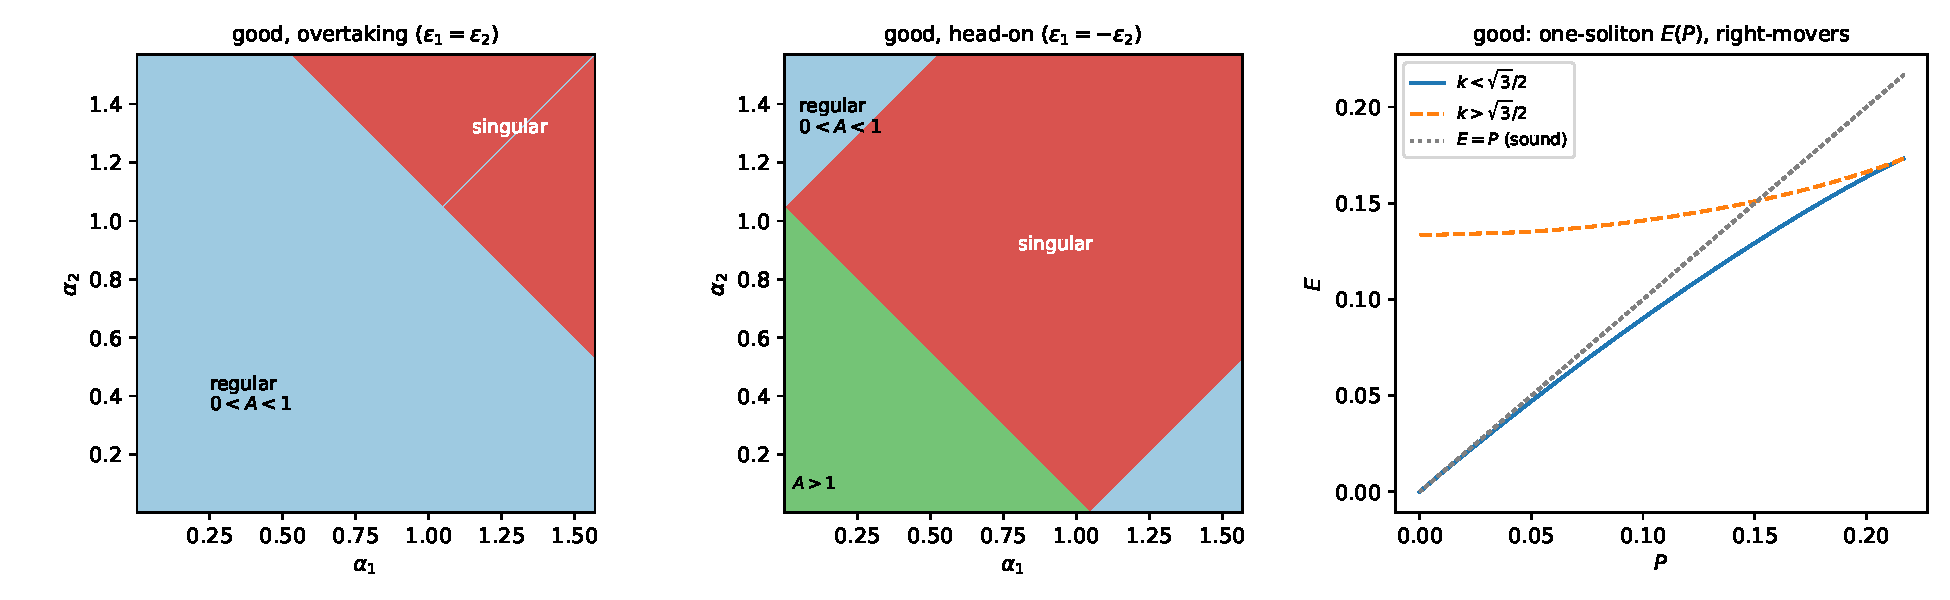
\includegraphics[width=\textwidth]{figures/regimes_and_dispersion.pdf}
\caption{\Good\ \emph{Left and centre:} regularity of the two-soliton solution in the $(\alpha_1,\alpha_2)$ plane for overtaking and head-on collisions. Red: singular ($A<0$). Blue: regular and repulsive ($0<A<1$). Green: regular and attractive ($A>1$). The boundaries are resonance lines. \emph{Right:} the one-soliton dispersion $E(P)$, with the light branch (solid) and heavy branch (dashed) meeting at the cusp $k=\sqrt3/2$. Figure from \scr{phase1/scripts/figures.py}.}\label{fig:regimes}
\end{figure}

\begin{proposition}[\Good, \Lc]\label{prop:regimes}
For the good equation (Fig.~\ref{fig:regimes}):
\begin{enumerate}
\item overtaking collisions are regular iff $\alpha_1+\alpha_2<\tfrac{2\pi}3$, and are then repulsive ($0<A<1$);
\item head-on collisions are regular and attractive ($A>1$) for $\alpha_1+\alpha_2<\tfrac\pi3$, regular and repulsive for $|\alpha_1-\alpha_2|>\tfrac\pi3$, and singular otherwise;
\item on each resonance line ($A=0$ or $\infty$) the sum or difference of the two solitons' $(k,\omega)$ satisfies the soliton dispersion relation, and the degenerate $\tau$-function describes a Y-junction in which two solitons merge or one splits.
\end{enumerate}
\chk{\scr{phase1/scripts/interaction_regimes.py} ($400^2$ grid)}
\end{proposition}
These regions agree with the conditions of Lambert, Musette and Kesteloot as quoted in \cite[(29)--(33)]{BD} \La/\Lc. In root language a resonance line is where two roots of different solitons coincide, so that $\ell_1=\ell_2$ \Lc.\chk{\scr{corrigan-zambon/defect_two_soliton_symplectic.py} (check 5)}

\paragraph{Position shifts.} For a physical collision, label the solitons so that soliton~1 starts to the left of soliton~2 with $v_1>v_2$. Then the asymptotic position shifts are
\begin{equation}\label{eq:shifts}
\Delta x_1=-k_1^{-1}\log A_{12},\qquad \Delta x_2=+k_2^{-1}\log A_{12}
\end{equation}
\Lc, checked against peak tracking of exact solutions in overtaking and attractive and repulsive head-on cases.\chk{\scr{phase1/scripts/interaction_regimes.py}} For small amplitudes in overtaking collisions, $\log A_{12}$ reduces to the KdV value $\log A_{\rm KdV}=2\log\big|\frac{k_1-k_2}{k_1+k_2}\big|$, so $\Delta x_1\sim-2k_1^{-1}\log\big|\frac{k_1-k_2}{k_1+k_2}\big|$ and $\Delta x_2\sim+2k_2^{-1}\log\big|\frac{k_1-k_2}{k_1+k_2}\big|$, while the head-on $\log A_{12}\to0$ \La~\cite{BD}/\Lc.\chk{\scr{paper/scripts/paper_draft2_checks.py} (check 3)}

\subsection{Breathers}\label{sec:breathers}

A breather is the real reduction $k_2=\bar k_1$, $\omega_2=\bar\omega_1$ of the two-soliton. It is regular iff $A(k,\bar k)>1$.

\begin{proposition}[\Both, \Lc]\label{prop:nobreather}
\begin{enumerate}
\item \Good\ For $\alpha=a+ib$, $A(k,\bar k)=\dfrac{1-3\cot^2a}{1+3\coth^2b}<\tfrac14$. Every Hirota breather of the good equation on the zero background is singular.
\item \Bad\ For $\beta_{1,2}=a\pm ib$ (Bogdan--Charkina's parametrisation $\kappa\pm ik=\sinh(a\pm ib)$), $A_{12}$ equals their $a_{12}$ \cite[(33)]{BC}, and the breather is regular iff $b>\pi/3$, which is their existence boundary $\pi/3<b\le\pi/2$ \La~\cite[(29)--(41)]{BC}.
\end{enumerate}
\chk{\scr{phase1/scripts/interaction_regimes.py} (good; grid and complex-$k$ scan); \scr{phase2/scripts/consistency_checks.py} (check 4, bad)}
\end{proposition}
Item~1 concerns the two-phase Hirota class on the zero background only. For the bad equation, breathers from the regular region of Charlier and Lenells are smooth for all $t$ and those from the singular region are singular at every $t$ \La~\cite[Lemma~A.4]{CL-SOL}.

\subsection{The good/bad dictionary}\label{sec:dictionary}

Table~\ref{tab:dict} collects the corresponding quantities. Results in this paper are stated for one equation or for both, as tagged.

\begin{table}[t]\centering\small
\caption{Dictionary between the good and bad equations. Entries are \Lc\ unless marked; the last three rows summarise Sections~\ref{sec:breathers}, \ref{sec:toda} and~\ref{sec:defects}.}\label{tab:dict}
\renewcommand{\arraystretch}{1.25}
\begin{tabular}{@{}>{\raggedright}p{3.1cm}>{\raggedright}p{5.6cm}>{\raggedright\arraybackslash}p{5.6cm}@{}}
\toprule
& good & bad\\\midrule
Equation & $u_{tt}=u_{xx}-u_{xxxx}-3(u^2)_{xx}$ & $v_{tt}=v_{xx}+v_{xxxx}+3(v^2)_{xx}$\\
Lagrangian & $\tfrac12\phi_t^2-\tfrac12\phi_x^2+\phi_x^3-\tfrac12\phi_{xx}^2$ & $\tfrac12\phi_t^2-\tfrac12\phi_x^2-\phi_x^3+\tfrac12\phi_{xx}^2$\\
Phonons & $\omega^2=q^2+q^4$ & $\omega^2=q^2-q^4$\\
Lax form & $q_L=\tfrac32u-\tfrac14$, $\tau=\sqrt3t$ & $q_L=\tfrac32v+\tfrac14$, $\tau=i\sqrt3t$\\
Rapidity & $k=\sin\alpha$, $\alpha\in(0,\frac\pi2)$ & $k=\sinh\beta$, $\beta>0$\\
Velocity & $v=\epsilon\cos\alpha$ (subsonic) & $v=\epsilon\cosh\beta$ (supersonic)\\
Spectral parameter & $\ell=-\epsilon\cos3\alpha$ & $\ell=\epsilon\cosh3\beta$\\
$M,\ \Pi$ & $2\sin\alpha,\ -\epsilon\sin2\alpha$ & $2\sinh\beta,\ -\epsilon\sinh2\beta$\\
$P$ & $\tfrac23\epsilon\sin^3\!\alpha\cos\alpha$ (bounded) & $\tfrac23\epsilon\sinh^3\!\beta\cosh\beta$\\
$E$ & $\tfrac2{15}k^3(5-4k^2)$ & $\tfrac2{15}k^3(5+4k^2)$\\
$dP/d(\text{rapidity})$ & $\tfrac23\epsilon\sin\alpha\sin3\alpha$ & $\tfrac23\epsilon\sinh\beta\sinh3\beta$\\
$A_{\rm ov}$; $A_{\rm ho}$ & \eqref{eq:Agood} & \eqref{eq:Abad}\\
Roots & real, $\tfrac12(\pm k+v/\sqrt3)$ & complex, $\tfrac12(iv/\sqrt3\pm k)$\\
Crossing map & $\alpha\to\alpha+\pi$ & $\beta\to\beta+i\pi$\\
Two-soliton regularity & regions, resonances (Prop.~\ref{prop:regimes}) & always regular, $0<A<1$\\
Regular breathers & none (Hirota class) & for $b>\pi/3$ \La~\cite{BC}\\
Toda continuum limit & --- & small amplitudes \La~\cite{Zak}\\
CZ type-I defects & exist \La~\cite{CZ} & no real type-I defect for $\lambda_{\rm CZ}\neq0$\\
\bottomrule
\end{tabular}
\end{table}

\begin{remark}[\Both, \Lc]\label{rem:continuation}
The substitution $\alpha=i\beta$ maps the good-equation soliton data to the bad ones according to
\[
(k,\,M,\,\Pi,\,P,\,E,\,\ell,\,v,\,A_{12})\big|_{\rm good}\ \longmapsto\ (ik,\,iM,\,i\Pi,\,-iP,\,-iE,\,-\ell,\,v,\,A_{12})\big|_{\rm bad},
\]
in both orientations; consequently the semiclassical phase~\eqref{eq:delta} below satisfies $\delta_{\rm good}(i\beta_1,i\beta_2)=-\delta_{\rm bad}(\beta_1,\beta_2)$.\chk{\scr{paper/scripts/paper_conventions_check.py} (check 5); the statement for $A_{12}$ is in \scr{phase1/scripts/interaction_regimes.py}} This explains why a single formula covers both equations. It is a statement about formulas, not a map between real solutions.
\end{remark}

%=====================================================================
\section{Canonical structure and exact symplecticity of scattering}\label{sec:canonical}

\subsection{Cross terms in the symplectic form}

Consider $N$ well-separated solitons at positions $X_j$ with parameters $k_j$, and normalise the potential by $\phi(-\infty)=c$. Then $\phi$ is a sum of kinks, $\phi_j$ rising from $0$ to $M_j$ across $X_j$, plus $c$.

\begin{proposition}[\Both, \Lc]\label{prop:Omega}
Up to exponentially small terms,
\begin{equation}\label{eq:Omega}
\Omega=d\Pi_{\rm tot}\wedge dc+\sum_jdP_j\wedge dX_j+\sum_{i\neq j}\big[X_i>X_j\big]\,d\Pi_i\wedge dM_j .
\end{equation}
\end{proposition}
The momentum density $\pi_i$ of soliton $i$ is localised at $X_i$, where $\phi_j$ equals $0$ or $M_j$ according to whether soliton $i$ is left or right of soliton $j$. This gives the cross terms. The diagonal term is the one-soliton result of Proposition~\ref{prop:EP}. In sine-Gordon the analogous cross term vanishes because the kink height $2\pi/\beta$ is fixed; here $M=2k$ varies \Lc.

\subsection{Scattering is symplectic only with the cross terms}

During a collision the parameters $k_j$ and the constant $c$ are conserved and $X_j\mapsto X_j+\Delta x_j$ with~\eqref{eq:shifts}. Soliton~1 starts on the left and ends on the right, so the cross term changes from $d\Pi_2\wedge dM_1$ to $d\Pi_1\wedge dM_2$.

\begin{proposition}[\Both, \Lc]\label{prop:symp}
The two-soliton scattering map preserves~\eqref{eq:Omega}:
\begin{equation}\label{eq:sympid}
\sum_jdP_j\wedge d\Delta x_j=d\Pi_2\wedge dM_1-d\Pi_1\wedge dM_2 .
\end{equation}
Without the cross terms the left side would have to vanish; it does not (for example it equals $19.79$ at $\beta=(0.9,0.3)$ in the bad equation).\chk{Bad: \scr{phase2/scripts/symplectic_scattering.py} (40 digits; overtaking and head-on, several points each). Good, regular region: \scr{phase2/scripts/consistency_checks.py} (double precision) and \scr{corrigan-zambon/defect_two_soliton_symplectic.py} (check 3, $10^{-40}$, with a defect present)}
\end{proposition}

Equation~\eqref{eq:sympid} shows that the naive rule $\Delta x_j=-\partial\delta/\partial P_j$ cannot hold for any function $\delta$: the shifts are not curl-free in the canonical momenta. The same identity holds on the Toda lattice in label coordinates (Proposition~\ref{prop:todalabel}).

\subsection{Darboux coordinates}

In each ordering region define
\begin{equation}\label{eq:darboux}
X_j'=X_j+\gamma_j\sum_{i\text{ left of }j}M_i,\qquad \gamma_j=\frac{d\Pi_j/dk_j}{dP_j/dk_j}
\end{equation}
\Lc. For the good equation $\gamma=-3\cos2\alpha/(\sin\alpha\sin3\alpha)$, which has a pole at the cusp \Lc.\chk{\scr{paper/scripts/paper_conventions_check.py} (check 9)} In these coordinates the cross terms are absorbed, and the shifts
\begin{equation}\label{eq:darbouxshifts}
\Delta X_1'=-\frac{\log A_{12}}{k_1}+\gamma_1M_2,\qquad \Delta X_2'=+\frac{\log A_{12}}{k_2}-\gamma_2M_1
\end{equation}
are curl-free in $(P_1,P_2)$ \Lc. Normalising $\phi$ at $+\infty$ instead gives the same in--out differences \Lc.\chk{\scr{phase2/scripts/semiclassical_phase.py}, \scr{phase2/scripts/consistency_checks.py} (check 1)}

%=====================================================================
\section{The semiclassical two-soliton phase}\label{sec:phase}

\subsection{The phase}

By stationary phase on two-particle wave packets, for a collision with incoming ordering $X_1<X_2$ ($v_1>v_2$) and away from $P_j'=0$, a phase $\delta(1,2)$ satisfying $\Delta X_j'=-\partial\delta(1,2)/\partial P_j$ gives the leading semiclassical S-matrix $S\simeq e^{i\delta/\hb}$ \La~\cite{FK}. We define $\delta(1,2)$ below as an antisymmetric function of the ordered pair of labels $(1,2)$, using the real principal logarithm on the regular region $A_{12}>0$ (excluding coincident solitons $k_1=k_2,\epsilon_1=\epsilon_2$ and resonance lines $A_{12}\in\{0,\infty\}$).

\begin{proposition}[\Both, \Lc]\label{prop:delta}
For overtaking and head-on collisions, in both equations,
\begin{equation}\label{eq:delta}
\boxed{\ \delta(1,2)=\tfrac29\,(\ell_1-\ell_2)\,\log A_{12}+\tfrac23\,M_1M_2\,(v_1-v_2)\ }
\end{equation}
with $\ell=-\epsilon\cos3\alpha$ (good) or $\ell=\epsilon\cosh3\beta$ (bad). The second term can be written $T_{12}\equiv\tfrac23M_1M_2(v_1-v_2)=-\tfrac23(\Pi_1M_2-\Pi_2M_1)$. For the good equation the statement holds in the regular region ($\alpha_j\neq\pi/3$, $A_{12}>0$).\chk{\scr{phase2/scripts/semiclassical_phase.py} (symbolic integration of the Darboux shifts); \scr{phase2/scripts/consistency_checks.py} (check 1, gradient test for both equations and orientations); \scr{paper/scripts/paper_draft2_checks.py} (check 8, symbolic root-polynomial proof)}
\end{proposition}

\paragraph{Analytic proof of the phase-gradient identity.} By~\eqref{eq:dP} and~\eqref{eq:cubic}, $dP_1=\tfrac29k_1\,d\ell_1$ in both equations \Lc. Differentiating~\eqref{eq:delta} with respect to the first soliton's parameter therefore gives $\partial_1\delta=(P_1'/k_1)\log A_{12}+\tfrac29(\ell_1-\ell_2)\partial_1\log A_{12}-\tfrac23(\Pi_1'M_2-\Pi_2M_1')$. In the root cross-ratio~\eqref{eq:crossratio}, each root satisfies $\ell(p)=-3\sqrt3p(1-4p^2)$, so for any pair of roots $(p_{1r},p_{2s})$ of solitons~$1$ and~$2$,
\[
\frac{\ell_1-\ell_2}{p_{1r}-p_{2s}}=-3\sqrt3\big[1-4(p_{1r}^2+p_{1r}p_{2s}+p_{2s}^2)\big],
\]
cancelling every pole of $\partial_1\log A_{12}$ identically \Lc. Taking the alternating sum over $r,s\in\{a,b\}$ and using $p_{ja}-p_{jb}=M_j/2$ and $p_{ja}^2-p_{jb}^2=-\Pi_j/(2\sqrt3)$ yields $\tfrac29(\ell_1-\ell_2)\partial_1\log A_{12}=-\tfrac13\Pi_1'M_2-\tfrac23\Pi_2M_1'$ \Lc. Adding $-\tfrac23(\Pi_1'M_2-\Pi_2M_1')$ cancels the $\Pi_2M_1'$ term and leaves $\partial_1\delta=(P_1'/k_1)\log A_{12}-\Pi_1'M_2=-P_1'\Delta X_1'$ \Lc.\chk{\scr{paper/scripts/paper_draft2_checks.py} (check 8)}

The remainder $T_{12}$ was first found by symbolic integration and then identified by this root identity \Lc. Three remarks:
\begin{itemize}
\item The dynamical part is (difference of spectral parameters)$\times\log A_{12}$. Because $dP=\tfrac29k\,d\ell$ and $(\ell_1-\ell_2)\partial_1\log A_{12}$ reduces to a polynomial in the roots, integration by parts closes and the tree-level phase is elementary: no dilogarithm appears at $O(\hb^{-1})$, in contrast to relativistic affine Toda theory \Lc~\cite{Hol93,Johnson}.
\item $T_{12}$ is an Aharonov--Bohm-like ``mutual statistics'' phase between objects carrying shift charge $\Pi$ and winding $M$ \Ld\ (interpretation).
\item The same structure, (difference of spectral parameters)$\times\log A$ minus a multiple of $\Pi_1M_2-\Pi_2M_1$, appears on the Toda lattice (Proposition~\ref{prop:todalabel}). We conjecture that it is universal for integrable models with a continuous kink charge, KdV included \Ld.
\end{itemize}

\subsection{Properties}

\begin{proposition}[\Both, \Lc]\label{prop:props}
\begin{enumerate}
\item \emph{Unitarity:} $\delta(1,2)=-\delta(2,1)$.
\item \emph{Crossing-type relation:} $\delta_{\rm ov}(\beta_1,\beta_2+i\pi)=-\delta_{\rm ho}(\beta_1,\beta_2)$ (bad) and $\delta_{\rm ov}(\alpha_1,\alpha_2+\pi)=-\delta_{\rm ho}(\alpha_1,\alpha_2)$ (good, regular head-on region). The shift maps a right-mover to a left-mover with $(k,M,\ell)\to(-k,-M,-\ell)$ and $A_{\rm ov}\to1/A_{\rm ho}$.
\item \Good\ \emph{Resonance lines:} where $A_{12}\to0$ or $\infty$ one has $\ell_1=\ell_2$, so $\delta\to T_{12}$ stays finite while the delays diverge logarithmically.
\item \Good\ \emph{Cusp:} at $\alpha_1=\pi/3$, $dP_1/d\alpha_1=0$ while $\partial_{\alpha_1}\delta=-\Pi_1'(\pi/3)M_2=-\epsilon_1M_2\neq0$; hence $\delta$ is smooth in $\alpha_1$ but has a square-root branch point $\delta(P_1,P_2)-\delta(P_{\rm cusp},P_2)\sim\mp\sqrt{2/\sqrt3}\,\epsilon_1M_2\sqrt{|P_{\rm cusp}-P_1|}$ as a function of $P_1$.
\end{enumerate}
\chk{Items 1--2: \scr{phase2/scripts/consistency_checks.py} (unitarity asserted; bad crossing printed) and \scr{paper/scripts/paper_conventions_check.py} (check 6, both asserted at 40 digits). Item 3: \scr{corrigan-zambon/defect_two_soliton_symplectic.py} (check 5, printed resonance-line limits). Item 4: \scr{corrigan-zambon/defect_two_soliton_symplectic.py} (check 5, soliton--defect cusp asserted) and \scr{paper/scripts/paper_draft2_checks.py} (check 8, two-body cusp square-root branch expansion asserted)}
\end{proposition}
Near the cusp the wave-packet derivation needs a uniform (Airy-type) treatment, and $\alpha$ or the root, rather than $P$, is the natural label \Ld. Past the resonance lines lie the Y-shaped solutions, which are outside the two-particle description.

\paragraph{Small amplitudes.} \Bad\ For overtaking collisions with $\beta_1/\beta_2=1.7$ fixed and $\beta_j\to0$, the ratio of the full phase derivative $\partial\delta/\partial\beta_1$ to the KdV-type term $2\beta_1\log A_{12}$ tends to $0.564246498175\ldots=1+2\beta_2/(\beta_1\log A_{\rm KdV})$, with $A_{\rm KdV}=(\frac{\beta_1-\beta_2}{\beta_1+\beta_2})^2$, while the cross-term-only ratio tends to $-0.435753501825\ldots$ \Lc. The cross-term contribution $-(d\Pi_1/d\beta_1)M_2\to4\beta_2$ to the phase derivative $\partial\delta/\partial\beta_1=-P_1'\Delta X_1'$ is therefore of the same order as the KdV-type term \Lc.\chk{\scr{phase2/scripts/consistency_checks.py} (check 6, reported as a finding); \scr{paper/scripts/paper_conventions_check.py} (check 7) and \scr{paper/scripts/paper_draft2_checks.py} (check 3), limit identified and asserted} The heuristic of Bonnemain and Doyon identifies the quantum phase derivative with $P'_{\rm GHD}\Delta x$, with $P_{\rm GHD}=\eta^2/2$ \Lb~\cite{BD}. It reproduces the dynamical term but misses the cross-term contribution \Lc; their classical hydrodynamics, which uses only $\Delta x$, is unaffected. \Both\ For head-on collisions $\delta\to4\beta_1\beta_2$, of which $\tfrac{16}3\beta_1\beta_2$ comes from $T_{12}$ and $-\tfrac43\beta_1\beta_2$ from the dynamical term (and likewise with $\alpha_j$ for the good equation) \Lc.\chk{\scr{paper/scripts/paper_conventions_check.py} (check 7)}

\subsection{Bad equation: breathers as spectral-parameter strings}\label{sec:BC}

Bogdan and Charkina compute the classical integrals and adiabatic invariant $I_{\rm br}$ of the Tajiri--Murakami breather of the bad equation, verifying $dE=(\tilde\omega/2\pi)\,dI_{\rm br}+V\,dP$ \La, and apply the semiclassical Bohr--Sommerfeld quantisation rule $I_{\rm br}=N\hb$ at large quantum number $N\gg1$ \Lb~\cite[(64)--(71)]{BC}.

\begin{proposition}[\Bad, \Lc]\label{prop:breather}
At $\beta_{1,2}=a\pm ib$,
\begin{equation}\label{eq:Ibr}
i\cdot\tfrac29(\ell_1-\ell_2)=-\tfrac49\sinh3a\,\sin3b=I_{\rm br},
\end{equation}
the Bogdan--Charkina classical adiabatic invariant \La~\cite[(64)]{BC}. Hence the coefficient of $\log A_{12}$ in~\eqref{eq:delta} is the breather action \Lc, and under the Bohr--Sommerfeld prescription $I_{\rm br}=N\hb$ \Lb\ breather quantisation reads
\begin{equation}\label{eq:string}
\ell_1-\ell_2=-\tfrac{9i}2\,N\hb,\qquad N\in\mathbb N .
\end{equation}
\chk{\scr{phase2/scripts/consistency_checks.py} (check 4, three parameter points, $10^{-16}$); \scr{paper/scripts/paper_conventions_check.py} (check 8, closed form)}
\end{proposition}

This ties the phase~\eqref{eq:delta}, built from Hirota shifts and the canonical symplectic form, to an independent classical action calculation in the literature \Lc. Equation~\eqref{eq:string} is a string condition in the spectral parameter, the form in which bound states appear in Bethe-ansatz solvable models. Extrapolating this semiclassical condition to finite $N$ suggests that an exact S-matrix has bound-state poles at $\ell_1-\ell_2\in-\tfrac{9i}2\hb\mathbb N$, possibly with a renormalised $\hb$ \Ld. The good equation has no regular Hirota breathers on the zero background (Proposition~\ref{prop:nobreather}), so there is no analogue of this check there.

\subsection{Bad equation: the classical limit of the quantum Toda Bethe ansatz}\label{sec:toda}

\paragraph{Set-up.} The Toda chain is $H=\sum_n(\tfrac12p_n^2+e^{-r_n})$ with $r_n=x_{n+1}-x_n$, mean spacing $a$ and $b=e^{-a/2}$. Its small-amplitude long-wave limit is the bad equation \La~\cite{Zak,BC}/\Lc.\chk{\scr{phase1/scripts/toda_limit.py}} The one-soliton is $e^{-r_n}=b^2[1+\sinh^2\kappa\,\sech^2(\kappa n-sbt\sinh\kappa)]$, with Toda direction sign $s=\pm1$ (distinct from the defect parameter $s=\sigma_0$ of Section~\ref{sec:defects}) and
\[
M=\sum(r_n-a)=-2\kappa,\qquad \Pi=\sum p_n=2sb\sinh\kappa,\qquad E=2b^2(\sinh\kappa\cosh\kappa-\kappa),
\]
where $E=\sum[\tfrac12p_n^2+e^{-r_n}-b^2+b^2(r_n-a)]$. The canonical form $\sum dp_n\wedge dx_n$ pulled back to $(\kappa,n_0)$ is $dP_n\wedge dn_0$ with label momentum $P_n=4sb(\kappa\cosh\kappa-\sinh\kappa)$, and $dE/dP_n=sb\sinh\kappa/\kappa$ is the signed label velocity \Lc.\chk{\scr{phase2/scripts/toda_soliton_classical.py}, \scr{phase2/scripts/toda_label_symplectic.py}; signed velocity verified for both $s=\pm1$ in \scr{paper/scripts/review_draft1_checks.py} and \scr{paper/scripts/paper_draft2_checks.py} (check 4a)} The two-soliton constant is $A_T=-\mathcal P_T(2\kappa_1-2\kappa_2,\omega_1-\omega_2)/\mathcal P_T(2\kappa_1+2\kappa_2,\omega_1+\omega_2)$ with $\mathcal P_T(K,W)=W^2-4b^2\sinh^2(K/2)$ and $\omega=2sb\sinh\kappa$ \Lc.\chk{\scr{phase1/scripts/toda_limit.py} (exact two-soliton in the lattice, $10^{-17}$); \scr{phase2/scripts/toda_label_symplectic.py}}

The relative two-body problem $(-\hb^2\partial_x^2+e^{-x})\psi=q^2\psi$ with incoming wave $e^{-iqx/\hb}$ has reflection amplitude $R=\Gamma(i\kappa)\hb^{2i\kappa}/\Gamma(-i\kappa)$, $\kappa=2q/\hb=\Delta p/\hb$ \La/\Lc.\chk{Verified from the exact Bessel eigenfunction $\psi(x)=K_{i\kappa}(2e^{-x/2}/\hb)$ and its $x\to+\infty$ asymptotics in \scr{paper/scripts/review_draft1_checks.py} and \scr{paper/scripts/paper_draft2_checks.py} (check 4b)} The asymptotic Bethe equations are $p_jL+\sum_l\Theta(p_j-p_l)=2\pi\hb I_j$ with $\Theta(D)=2\hb\,\mathrm{Im}\log\Gamma(1+iD/\hb)+2D\log\hb$ (using the unwrapped logarithm branch), whose classical limit is $2(D\log|D|-D)$; the method is that of Sutherland and Mertens \Lb~\cite{Sutherland,Mertens}.

\begin{proposition}[\eqtag{red!60!black}{Toda $\to$ bad}, \Lc]\label{prop:todaBA}
As $\hb\to0$:
\begin{enumerate}
\item the ground-state quasi-momenta fill $[-2b,2b]$ with the arcsine density of total weight $1/a$, which is the Lax spectrum of the static lattice, and reproduce the ground-state energy per particle $b^2$;
\item a particle excitation at $p=2sb\cosh\kappa$, the soliton's Lax eigenvalue, has dressed momentum $P_n/a$ and dressed energy, relative to the edge, equal to the soliton energy $E$;
\item the exact classical physical-frame shifts are $\Delta x_1=a\Delta n_1+M_2$ and $\Delta x_2=a\Delta n_2-M_1$, the extra terms being the displacement caused by the other soliton's compression; they are given by $\Delta x_2=-\partial\Phi(1|2)/\partial P_2$ and $\Delta x_1=+\partial\Phi(2|1)/\partial P_1$, where $\Phi(1|2)$ is the dressed Bethe phase of excitation~1 in the presence of~2;
\item $\Phi(1|2)+\Phi(2|1)$ is not separable; its mixed derivative with respect to $(\kappa_1,\kappa_2)$ equals $M_1'(P_{n2}'/a-\Pi_2')+M_2'(P_{n1}'/a-\Pi_1')$ (primes denoting $d/d\kappa_j$), i.e.\ the Bethe ansatz carries precisely the cross terms of Proposition~\ref{prop:Omega}.
\end{enumerate}
\chk{\scr{phase2/scripts/toda_bethe_classical.py} ($10^{-8}$, Chebyshev method); \scr{phase2/scripts/toda_dressed_phase_check.py}; \scr{phase2/scripts/toda_ba_vs_label.py}}
\end{proposition}

\begin{proposition}[\eqtag{red!60!black}{Toda $\to$ bad}, \Lc]\label{prop:todalabel}
In the Toda label frame, two-soliton scattering satisfies $\sum_jdP_{n,j}\wedge d\Delta n_j=d\Pi_2\wedge dM_1-d\Pi_1\wedge dM_2$ (30 digits), the analogue of~\eqref{eq:sympid}. The Darboux phase is
\begin{equation}\label{eq:deltaT}
\delta_T=(p_1-p_2)\log A_T+M_1M_2(v_1-v_2)=(p_1-p_2)\log A_T-(\Pi_1M_2-\Pi_2M_1),
\end{equation}
with $p=2sb\cosh\kappa$ and $v=sb\sinh\kappa/\kappa$ the signed label velocity.\chk{\scr{phase2/scripts/toda_label_symplectic.py} (symplectic identity); \scr{phase2/scripts/toda_scaling_fast.py} (remainder fitted to $M_1M_2(v_1-v_2)$, ratio $1$ to ten digits); \scr{phase2/scripts/toda_ba_vs_label.py} ($\Phi(1|2)=\delta_T+M_1(P_{n2}/a-\Pi_2)+f(\kappa_1)$ and its mirror, to machine precision)}
\end{proposition}

\begin{proposition}[\eqtag{red!60!black}{Toda $\to$ bad}, \Lc]\label{prop:todascaling}
With $\kappa_j=\sqrt3\beta_j\to0$ and action scale $S_{\rm Toda}=3b\,S_{\rm Bouss}$,
\[
\delta_T/(3b\,\delta_{\rm bad})\to1
\]
for overtaking \emph{and} head-on collisions; the error is $\approx6\times10^{-6}$ at $\beta\sim3\times10^{-3}$.\chk{\scr{phase2/scripts/toda_scaling_fast.py}}
\end{proposition}

In head-on collisions the leading Boussinesq phase $4\beta_1\beta_2$ is dominated by the topological term ($\tfrac{16}3\beta_1\beta_2$ against $-\tfrac43\beta_1\beta_2$). Agreement in that channel therefore confirms the topological term of~\eqref{eq:delta} from an exactly solvable quantum model \Lc. The split between the two terms of~\eqref{eq:deltaT} is not preserved by the scaling limit; only their sum is \Lc.

\paragraph{Limitation.} The Toda continuum limit produces the bad equation only at leading order in amplitude, so Toda tests~\eqref{eq:delta} only as $\beta\to0$. Finite-$\beta$ solitons have widths comparable to the dispersion length, where the bad equation is ill-posed and Toda and Boussinesq differ at $O(1)$ \Lc. An exact S-matrix for finite-amplitude bad solitons would require a quantum regularisation that agrees with Boussinesq at the dispersion scale; we know of none \Ld. The $O(\hb)$ Toda corrections and the Fermi-edge double-scaling limit are discussed in Section~\ref{sec:fermi}.

%=====================================================================
\section{Integrable defects at tree level}\label{sec:defects}

\Good\ Throughout this section the bulk theory is the good equation.

\subsection{Corrigan--Zambon defects}

Corrigan and Zambon construct integrable type-I defects for the good Boussinesq equation, with a defect Lagrangian $D=u_tF+v_tG+H$ at $x_0$ coupling the fields $u$ ($x<x_0$) and $v$ ($x>x_0$) \La~\cite{CZ}. Within their ansatz, with the nonlinear term present, the defect coefficients are forced to be imaginary when the dispersion has the bad sign, so \emph{no real type-I defect of this family exists for the bad equation}; for the linear equation real defects do exist \Lc.\chk{\scr{corrigan-zambon/defect_check.py} (sewing conditions and momentum flux rederived from the action with the dispersion sign kept symbolic)} A type-II defect for the bad equation is not excluded \Ld. This is why defects are a good-equation topic.

\paragraph{Dictionary.} With $c=\lambda=\kappa=1$ in \cite{CZ}, $u_{\rm CZ}=-3\phi$, $L_{\rm CZ}=9\mathcal L$, $P_{\rm CZ}=9P$, $\gamma=\sech\theta=k$ and $\nu=\tanh\theta=\epsilon\cos\alpha$ \Lc.\chk{\scr{corrigan-zambon/defect_transmission_phase.py} (check 1)} The defect has parameter $s=\sigma_0$ and orientation $\eta=\pm1$ (CZ's $\alpha_{\rm CZ}=\eta/\sqrt3$, $\beta_{\rm CZ}=2\eta/\sqrt3$, obeying $\beta_{\rm CZ}^2-\alpha_{\rm CZ}^2=1$ \La~\cite[(3.22),(3.37)]{CZ}). The sewing conditions were rederived from the action and checked on the exact solutions \Lc.\chk{\scr{corrigan-zambon/verify_defect_solutions.py} ($10^{-28}$--$10^{-31}$ away from poles)} One- and two-soliton solutions are purely transmitted, each $e^{\theta_j}$ being multiplied by
\begin{equation}\label{eq:zCZ}
z=\frac{\sinh\theta+s\cosh\theta-\eta\sqrt3}{\sinh\theta+s\cosh\theta+\eta\sqrt3}
\end{equation}
on the far side \La~\cite[(5.5),(5.11)]{CZ}.

\begin{proposition}[\Good, \Lc]\label{prop:z}
With the soliton roots~\eqref{eq:roots} and the \emph{defect root} $q=-s/(2\sqrt3)$,
\begin{equation}\label{eq:zroot}
z=\Big(\frac{p_b-q}{p_a-q}\Big)^{\eta},\qquad \ell(q)=\tfrac12(3s-s^3).
\end{equation}
Formally $z^{-\eta}$ is the cross-ratio~\eqref{eq:crossratio} of the soliton with the pair $(q,\infty)$: the defect behaves like half a soliton. The transmitted solution is regular iff $z\in(0,\infty)$, i.e.\ $q\notin[p_b,p_a]$; for $|s|>2$ every soliton is regular, in agreement with \cite{CZ} \La. The delay is $\Delta x=-k^{-1}\log z^\epsilon$.\chk{\scr{corrigan-zambon/defect_transmission_phase.py} (checks 2--3; delay from peak positions, 16 cases, $10^{-39}$)}
\end{proposition}

Corrigan and Zambon remark that no factor of the two-soliton constant seems closely related to $z$ \La; in root variables the relation is transparent.

\subsection{Symplectic structure with a defect}

The defect adds $F\,\delta u+G\,\delta v$ at $x_0$ to the canonical one-form $\Theta$. Asymptotically $F\to f(u,v)$ and $G\to g(u,v)$, so with $\Omega=d\Theta$ the defect contributes $\Omega_D=d(f\,du+g\,dv)|_{x_0}=(g_u-f_v)\,du\wedge dv|_{x_0}$ \Lc. On every fixed vacuum sector $u-v$ at $x_0$ is a discrete label, so $du=dv$ and $\Omega_D=0$ \Lc.\chk{\scr{corrigan-zambon/defect_transmission_phase.py} (check 6); two-form sign checked in \scr{paper/scripts/review_draft1_checks.py} and \scr{paper/scripts/paper_draft2_checks.py} (check 5)} Hence the type-I defect contributes no continuous canonical pair on a fixed vacuum sector and introduces no soliton--defect cross terms (this does not imply the absence of localised defect energy or momentum).\footnote{We use the shift-invariant gauge $f=g=-\sigma^2/(4\mu)$ ($\mu=1$, $\sigma=v-u+\eta\sqrt3\kappa$) with $g_u-f_v=\sigma$, in which the total $\Pi$ is conserved through the defect. The example gauge printed in \cite[(3.43),(3.47)]{CZ} gives $2\sigma$; this looks like a typo there \Lc\ (\scr{corrigan-zambon/README.md}).} For one soliton, any map $X\mapsto X+\Delta x(P)$ is then symplectic, so the content lies in the phase and in the multi-soliton case.

\subsection{The transmission phase}

\begin{proposition}[\Good, \Lc]\label{prop:dD}
With $\Delta x=-\partial\delta_D/\partial P$, for all $\epsilon,\eta=\pm1$ and all $s$ in the regular region,
\begin{equation}\label{eq:dD}
\boxed{\ \delta_D=\tfrac29\big(\ell-\ell_D\big)\log z^{\epsilon}-\tfrac23\big(\Pi M_D-\Pi_DM\big)\ },\qquad
\ell_D=\ell(q),\quad M_D=\epsilon\eta\,q,\quad \Pi_D=\epsilon\eta\,\frac{s^2-2}{2\sqrt3},
\end{equation}
up to an additive $s$-dependent constant that the classical data do not fix. The two orientations are semiclassically inverse: $\delta_D(-\eta)=-\delta_D(\eta)$.\chk{\scr{corrigan-zambon/defect_transmission_phase.py} (check 4, 40 digits)}
\end{proposition}

The defect enters like a second particle with spectral parameter $\ell(q)$ and effective coefficients $(M_D,\Pi_D)$ \Lc\ (formula); the particle reading is \Ld. In CZ's notation $\ell_D=-\sqrt3\,\eta\rho_0$, so the defect's spectral parameter is its constant $\rho_0$ \Lc. Since $M_D$ and $\Pi_D$ depend on $\epsilon$, they are effective coefficients of a mutual-statistics term rather than intrinsic defect charges.

\subsection{Two solitons and a defect}

\begin{proposition}[\Good, \Lc]\label{prop:2sD}
For two solitons crossing a defect (overtaking and head-on, both orientations, $s$ of both signs, regular region):
\begin{enumerate}
\item the position shifts are $\Delta x_j=\Delta x_j^{\rm ss}+\Delta x_j^{D}$, identical whether the soliton--soliton collision happens left or right of the defect;
\item the identity~\eqref{eq:sympid} holds with the soliton--soliton cross terms and no defect cross terms;
\item in the Darboux frame~\eqref{eq:darboux}, $\Delta x_j'=-\partial_{P_j}(\delta_{12}+\delta_{1D}+\delta_{2D})$.
\end{enumerate}
\chk{\scr{corrigan-zambon/defect_two_soliton_symplectic.py} (checks 2--4; shifts from peak positions at $t=\pm1000$ to $10^{-27}$; identities to $10^{-40}$)}
\end{proposition}
Semiclassically the soliton--soliton--defect amplitude therefore factorises as $S_{12}T_1T_2$, and the compatibility relation $T_1T_2S_{12}=S_{12}T_2T_1$ is automatic for diagonal, purely transmitting scattering. The nontrivial content is that the defect shifts do not depend on the other soliton, and that the Darboux corrections are unaffected by the defect because $\Omega_D=0$ \Lc.

\subsection{Vacua, absorption and linear stability}

The static defect vacua are $\sigma\in\{s,\sigma_+,\sigma_-\}$ with $\sigma_\pm^2+s\sigma_\pm+s^2=3$, equivalently the roots of $P_{\rm vac}(\sigma)\equiv\sigma^3-3\sigma+s(3-s^2)=0$ \Lc. Writing $\sigma=-2\sqrt3\,q'$, this reads $q'^2+qq'+q^2=\tfrac14$: the excited vacua $\sigma_\pm$ are the \emph{other two roots of the KP triple containing $q$} \Lc. Since $\sigma_\pm^2+s\sigma_\pm+s^2-3$ has discriminant $\Delta=3(4-s^2)$ and $(s-\sigma_+)(s-\sigma_-)=3(s^2-1)$, all three vacua of the triple are real and distinct iff $|s|<2$ and $s\neq\pm1$; at $|s|=2$ or $s=\pm1$ two roots coincide (at $\eta s=2$ they coincide at the marginal point $\eta\sigma=-1$), while for $|s|>2$ the excited roots $\sigma_\pm$ are nonreal complex conjugates, leaving $\sigma=s$ as the unique real vacuum \Lc.\chk{\scr{paper/scripts/review_draft1_checks.py}; \scr{paper/scripts/paper_draft2_checks.py} (check 6)} Absorption ($z\in\{0,\infty\}$) occurs iff $q=p_a$ or $q=p_b$ (which requires $|s|<2$) \La~\cite{CZ}/\Lc. The defect with root $q$ then absorbs the soliton $(q,p)$ and becomes the defect with root $p$ in the same triple, with exact energy--momentum balance between the soliton and the jump of the defect's $(E_D,P_D)$ \Lc.\chk{\scr{corrigan-zambon/defect_transmission_phase.py} (check 5, $10^{-40}$)} On an absorption line $\ell=\ell(q)$, so $\delta_D$ stays finite while the delay diverges logarithmically \Lc.\chk{\scr{corrigan-zambon/defect_two_soliton_symplectic.py} (check 5)}

\begin{proposition}[\Good, \Lc/\Ld]\label{prop:stab}
Linearise the sewing conditions about a real static vacuum $\sigma_{\rm vac}$; the bulk equation becomes $a_{tt}=a_{xx}-a_{xxxx}$.
\begin{enumerate}
\item On every real vacuum phonons are purely transmitted, $R=0$, $|T|=1$, with $T$ equal to CZ's linear-defect formula \cite[(4.6)]{CZ} at $\sigma_0\to\sigma_{\rm vac}$ \Lc.
\item Numerical searches over the spectral plane find a localised growing mode for $\eta\,\sigma_{\rm vac}>-1$ and find no growing mode for $\eta\,\sigma_{\rm vac}<-1$ (with $\eta\,\sigma_{\rm vac}=-1$ marginal) \Lc; that no growing mode exists anywhere in the complex plane for $\eta\,\sigma_{\rm vac}<-1$ is a completeness statement beyond the finite grid \Ld. Every growing mode found has zero conserved energy; the defect's quadratic energy is indefinite \Lc.
\item For $|s|<2$ and $s\neq\pm1$, the cubic $P_{\rm vac}(\sigma)=\sigma^3-3\sigma+s(3-s^2)$ has derivative $P_{\rm vac}'(\sigma)=3(\sigma^2-1)$ and satisfies $P_{\rm vac}(-1)=(2-s)(1+s)^2>0$ and $P_{\rm vac}(+1)=-(2+s)(1-s)^2<0$; by Rolle's theorem its three distinct real vacua lie in $(-\infty,-1)$, $(-1,1)$ and $(1,\infty)$, so \emph{exactly one vacuum per distinct real triple satisfies the strict stability condition $\eta\,\sigma_{\rm vac}<-1$} \Lc.
\end{enumerate}
\chk{\scr{corrigan-zambon/defect_vacuum_stability.py} (fine scan of the imaginary axis plus Newton iteration from a complex grid); Rolle's-theorem separation and threshold cases checked symbolically in \scr{paper/scripts/review_draft1_checks.py} and \scr{paper/scripts/paper_draft2_checks.py} (check 6)}
\end{proposition}

Consequently, within the sampled mode search, a defect with ground vacuum $\sigma=s$ is strictly linearly stable for $\eta s<-1$ (marginal at $\eta s=-1$) and linearly unstable for $\eta s>-1$ \Lc/\Ld. Corrigan and Zambon's illustrative example ($s=0.5$, $\eta=+1$) has a linearly unstable ground vacuum, with growth rate $\approx0.4999$; its exact soliton solutions are unaffected \Lc. Soliton absorption by a strictly stable ground defect is possible only for $-2<\eta s<-1$, where all three vacua of the triple are real and distinct; in that range both excited vacua $\sigma_\pm$ have $\eta\sigma_\pm>-1$ and are linearly unstable \Lc, so the absorbed soliton leaves the defect in an unstable state, presumably a resonance that re-emits \Ld. (For $\eta s<-2$ the ground vacuum is stable and the two excited roots are nonreal, so no real soliton is absorbed \Lc.)

\subsection{Tree-level fusion}

\begin{proposition}[\Good, \Lc]\label{prop:fusion}
Let $|s|<2$ ($s\neq\pm1$) and let a defect with root $q$ absorb the soliton $S=\{q,q'\}$ (with $k_S=|q-q'|$ and velocity $v_S=\sqrt3(q+q')$) and become the defect with root $q'$. For the displayed zero-constant representatives~\eqref{eq:dD} and every test soliton~3 in the regular region,
\begin{equation}\label{eq:fusion}
\delta_D^{(q')}(3)-\delta_D^{(q)}(3)=\rho\,\big[\delta(3,S)+M_S\Pi_3\big],\qquad\rho=\epsilon_3\eta\sgn(q-q') .
\end{equation}
The term $M_S\Pi_3$ is the cross term of soliton~3 with the $\phi$-jump $M_S$ stored in the excited defect. Shifting $\delta_D^{(q)}\mapsto\delta_D^{(q)}+C(q)$ by an $s$-dependent constant leaves the classical delay $\Delta x=-\partial_P\delta_D$ unchanged and adds $C(q')-C(q)$ to the left-hand side of~\eqref{eq:fusion}.\chk{\scr{phase2/scripts/defect_smatrix_good_continuation.py} (check 4; 12 triangles, $10^{-40}$); oriented sign $\rho=\epsilon_3\eta\sgn(q-q')$ and additive-constant shift verified in \scr{paper/scripts/review_draft1_checks.py} and \scr{paper/scripts/paper_draft2_checks.py} (check 7)}
\end{proposition}

Identity~\eqref{eq:fusion} is a classical, leading-order soliton--soliton--defect bootstrap for the zero-constant representatives~\eqref{eq:dD} \Lc; fixing the absolute $s$-dependent phase constant requires quantum input \Ld. All three solitons of one KP triple have the same $\ell$. Promoting~\eqref{eq:fusion} to an exact relation between quantum amplitudes would require the excited defect vacua to be asymptotic states. For $-2<\eta s<-1$, Proposition~\ref{prop:stab} shows that they are linearly unstable, so any quantum fusion argument built on~\eqref{eq:fusion} is heuristic \Ld. We examine the defect's localised charges, linearised sewing determinant, one-loop spectral trace and fusion obstructions next.

\subsection{Localised defect charges, one-loop renormalisation and fusion obstructions}\label{sec:defq}

\paragraph{Classical defect charges and absorption balance.} In project normalisation ($\mathcal L_{\rm CZ}=9\mathcal L_{\rm good}$, $u_{\rm CZ}=-3\phi_L$, $v_{\rm CZ}=-3\phi_R$, $\alpha_{\rm CZ}=\eta/\sqrt3$, $\beta_{\rm CZ}=2\eta/\sqrt3$, $\sigma=s-\sqrt3\eta(\phi_L-\phi_R)$ at $x=0$), the defect Lagrangian is $D_{\rm proj}=\phi_{L,t}F_{\rm proj}+\phi_{R,t}G_{\rm proj}-E_D$ with $F_{\rm proj}=-\tfrac13F_{\rm CZ}$ and $G_{\rm proj}=-\tfrac13G_{\rm CZ}$ \Lc. Varying $\int_{x<0}\mathcal L_{\rm good}+\int_{x>0}\mathcal L_{\rm good}+\int D_{\rm proj}\,dt$ yields the sewing conditions at $x=0$, under which all four total charges $(E_{\rm bulk}+E_D,P_{\rm bulk}+P_D,\Pi_{\rm bulk}+\Pi_D,M_{\rm bulk}+M_D)$ are conserved identically on the sewing manifold \Lc, with localised defect charges
\begin{equation}\label{eq:defcharges}
\begin{aligned}
E_D&=-\frac{\eta}{\sqrt3}\sigma(\phi_{L,x}^2+\phi_{L,x}\phi_{R,x}+\phi_{R,x}^2)+\frac13\rho(\sigma)(\phi_{L,x}+\phi_{R,x})-\frac19\tau(\sigma),\\
P_D&=-\frac{\eta}{2\sqrt3}(\phi_{L,x}^2+4\phi_{L,x}\phi_{R,x}+\phi_{R,x}^2)+\frac19h(\sigma),\\
\Pi_D&=F_{\rm proj}+G_{\rm proj}=\sqrt3\eta(\phi_{L,x}+\phi_{R,x})+\frac{\sqrt3\eta}6\sigma^2,\qquad
M_D=\phi_R(0^+,t)-\phi_L(0^-,t)=\frac{\sigma-s}{\sqrt3\eta}
\end{aligned}
\end{equation}
\Lc.\chk{\scr{phase2/scripts/defq_classical_charges.py}; \scr{phase2/scripts/audit_defq.py}; \scr{paper/scripts/paper_draft3_checks.py} (check 1a). In \cite[(3.49)]{CZ}, $P_{D,{\rm CZ}}$ already incorporates $-u_{{\rm CZ},x}F_{\rm CZ}-v_{{\rm CZ},x}G_{\rm CZ}$, so $P_D=P_{D,{\rm CZ}}/9$ is free of time derivatives \Lc.}
On a static vacuum $\sigma_i=-2\sqrt3\,q_i$ ($\phi_{L,x}=\phi_{R,x}=0$), across any edge $S_i=\{q_i,q_{i+1}\}$ of a KP triple $q_i^2+q_iq_{i+1}+q_{i+1}^2=\tfrac14$, the vacuum jumps of all four charges~\eqref{eq:defcharges} factorise modulo the KP circle into $\Delta(E_D^{\rm vac},P_D^{\rm vac},\Pi_D^{\rm vac},M_D^{\rm vac})_{q_i\to q_{i+1}}=\rho_i\,(E,P,\Pi,M)_{S_i}$ with $\rho_i=\eta\sgn(q_i-q_{i+1})$ \Lc.\chk{\scr{phase2/scripts/defq_classical_charges.py} (symbolic and transmission quadrature); \scr{phase2/scripts/audit_defq.py} (50-digit time-dependent conservation on genuine $z=0$ absorption, correcting an extra $\eta$ factor in the numerical absorption input of \scr{phase2/scripts/defq_classical_charges.py}); \scr{paper/scripts/paper_draft3_checks.py} (check 1a)}

\paragraph{Linearised sewing determinant and growing-mode counts.} For a localised mode $e^{gt}$ on a static vacuum $\sigma_{\rm vac}=-2\sqrt3\,q_{\rm vac}$ with decaying spatial exponents $\kappa_1,\kappa_2$ ($\operatorname{Re}\kappa_{1,2}>0$, $S=\kappa_1+\kappa_2>1$, $\kappa_1\kappa_2=(S^2+1)/2$ and $g=(S^2-1)/2>0$), the off-shell reduced $4\times4$ linearised sewing determinant depends on $c\equiv s_{\rm eff}=\eta\sigma_{\rm vac}$ and factorises as
\begin{equation}\label{eq:detMdef}
\frac{\det M}{(\kappa_1-\kappa_2)^2}=-\tfrac23S^2(S^2-1)P_-(S;c)P_+(S;c),\qquad
P_\mp(S;c)=S^2-\frac{\sqrt3\mp1}2cS+\frac{c^2-2\mp\sqrt3}2
\end{equation}
\Lc.\chk{\scr{phase2/scripts/audit_frames_defects.py}; \scr{phase2/scripts/defq_oneloop_renorm.py}; \scr{phase2/scripts/audit_defq.py}; \scr{paper/scripts/paper_draft3_checks.py} (check 1b). The prefactor $-\tfrac23$ corrects a missing factor of $16$ in an earlier note (\scr{phase2/oneloop_defect_phase.pdf}).}
At the continuum threshold $S=1$, $P_\mp(1;c)=\tfrac12(c\pm1)(c-\sqrt3)$, so an admissible root ($S>1$) enters at $c=-1$ (from $P_-$) and a second enters at $c=+1$ (from $P_+$), while at $c=\sqrt3$ the second root passes through $S=1$ in a branch switch from $P_-$ to $P_+$ where the remaining positive growth rate is $g(\sqrt3)=\sqrt3/4$ \Lc.\chk{\scr{phase2/scripts/audit_defq.py} and \scr{paper/scripts/paper_draft3_checks.py} (check 1b), correcting a misprinted value $(2\sqrt3-1)/8$ in \scr{phase2/defq_charges_fusion.pdf}} Across any nondegenerate real KP triple ($|s|<2$, $s\neq\pm1$), the sorted admissible growing-mode counts of the three vacua are $(0,1,2)$ generically and $(0,1,1)$ on the triple containing $c=\sqrt3$, so no elementary single-soliton absorption step connects two linearly stable defect vacua \Lc.

\paragraph{One-loop spectral trace and UV boundary counterterm.} With the reflectionless phonon transmission phase $\theta_D(q;c)$ ($z_{\rm ph}(\pm\infty)=e^{-2\pi i\eta/3}$) and vacuum mode covariance $\langle a^2\rangle_q=\tfrac1{4\pi\omega(q)}$ ($\omega(q)=|q|\sqrt{1+q^2}$), the quadratic localised defect momentum $P_{D,2}$ and the boundary symplectic pairing of $D_2=a_tF_1+b_tG_1-E_{D,2}$ satisfy the exact pointwise identities
\begin{equation}\label{eq:PD2trace}
\begin{aligned}
\langle P_{D,2}\rangle_q+\langle P_{D,2}\rangle_{-q}&=\frac{q}{4\pi}\big(\theta_D'(q)-\theta_D'(-q)\big)
=\frac{\sqrt3\eta q\,\big(2(\sigma_{\rm vac}^2-2)q^2+\sigma_{\rm vac}^2-1\big)}{\pi\sqrt{1+q^2}\,\big(16q^4+4(\sigma_{\rm vac}^2+2)q^2+(\sigma_{\rm vac}^2-1)^2\big)},\\
+\big(\langle a_tF_1+b_tG_1\rangle_q+\langle a_tF_1+b_tG_1\rangle_{-q}\big)&=\frac{\omega(q)}{4\pi}\big(\theta_D'(q)+\theta_D'(-q)\big)
\end{aligned}
\end{equation}
\Lc.\chk{\scr{phase2/scripts/defq_oneloop_renorm.py}; \scr{phase2/scripts/audit_defq.py} (noting the $+$-sign on the second line and the $\langle a^2\rangle_q=1/(4\pi\omega)$ normalisation); \scr{paper/scripts/paper_draft3_checks.py} (check 1c)}
In the equal-mode-count cutoff $\Lambda$ ($T=\sqrt{1+\Lambda^2}$ and $S_D=-\tfrac12\eta\sqrt3\sigma_{\rm vac}$), the regulated defect Casimir energy $E_D^{\rm mode}(\Lambda)=E_D^{\rm dens}(\Lambda)-B_D(\Lambda)=\frac{S_D}{\pi}(T-1)+\Delta E_D^{\rm ren}+O(\Lambda^{-1})$ diverges linearly \Lc. Because the open-half-line bulk tadpole $\propto\int_{x\neq0}\phi_x\,dx$ vanishes on every constant defect vacuum, cancelling this UV divergence requires a localised boundary counterterm
\begin{equation}\label{eq:defUVct}
\delta E_D^{\rm ct}(\Lambda)=-\frac{S_D}{\pi}(T-1)+\delta E_D^{\rm fin}
=\frac{\eta\sqrt3\,s}{2\pi}(T-1)+\frac3{2\pi}(T-1)M_D+\delta E_D^{\rm fin}
\end{equation}
(or renormalisation of the defect parameter $s\mapsto s+\hb\,\delta s_1$), whose $M_D$ term completes the bulk topological tadpole across the potential jump at $x=0$ \Lc;\chk{\scr{phase2/scripts/defq_oneloop_renorm.py}; \scr{phase2/scripts/audit_defq.py}; \scr{paper/scripts/paper_draft3_checks.py} (check 1c)} fixing the finite boundary scheme $\delta s_1$ and constructing the full quantum boundary theory remain open \Ld.

\paragraph{Qualifications and obstructions to one-loop KP-triangle fusion.} While the algebraic continuum phase integrals and test-soliton delay shifts close around any KP triangle $\{q_1,q_2,q_3\}$ at fixed bare root parameters \Lc, promoting tree-level fusion~\eqref{eq:fusion} to a physical $O(\hb^0)$ bootstrap constraint on the two-soliton S-matrix is obstructed by three facts \Lc/\Ld:\chk{\scr{phase2/scripts/defq_absorption_fusion.py}; \scr{phase2/scripts/audit_defq.py}; \scr{paper/scripts/paper_draft3_checks.py} (check 1d)}
\begin{enumerate}
\item \emph{Intermediate vacuum instability:} Factoring a composite process $D(q_{\rm st})+S_{12}+S_{23}\to D(q_{\rm st})+S_{13}$ on the unique stable vacuum $q_{\rm st}$ into elementary single-soliton steps traverses the two linearly unstable vacua of the triple \Lc\ (whether a resonance continuation exists is \Ld).
\item \emph{Canonical-charge triangle holonomy:} Under minimal tadpole subtraction ($\delta s_1=0$), the two-root dipole defect shifts match the mode-sum soliton shifts $(\Delta E_1^{\rm ren},\Delta P_{\rm mode})$ and sum to zero around any closed KP triangle \Lc. By contrast, the co-moving canonical shifts $(\Delta E_{\rm can},\Delta P_{\rm can})$ have nonzero directed triangle holonomy on sampled nondegenerate triples (for example $(+0.31753733,+0.16558489)$ at $q_1=-0.20$, $\eta=+1$) \Lc. Because any single-valued vertex assignment telescopes to zero around a closed triangle, no single-valued defect state-charge counterterm can balance $(\Delta E_{\rm can},\Delta P_{\rm can})$ at unshifted absorption rapidities on such a triangle \Lc\ (universal nonvanishing is sampled rather than analytically proved, while an $O(\hb)$ kinematic shift $\delta\alpha_{S_i}=(\Delta P_{\rm mode}-\Delta P_{\rm can})/P_{\rm cl}'(S_i)$ restores closure \Lc; deriving such a shift from quantum sewing is \Ld).
\item \emph{Absorbed-soliton momentum remainder:} Holding the physical momenta of both colliding solitons fixed in $S(3,S_i)$ adds the second Taylor term $\sum_{i=1}^3\rho_{{\rm tree},i}\Delta X_{S_i}(3,S_i)\Delta P(S_i)=\sum_{i=1}^3\big(\frac{\Delta P(S_{i-1})}{k_{S_{i-1}}}-\frac{\Delta P(S_i)}{k_{S_i}}\big)\log|z(3;q_i,\eta)|$, which is nonzero at tested points ($-0.77421697$ for $\Delta P_{\rm mode}$ and $-1.73701087$ for $\Delta P_{\rm can}$ at $q_1=-0.20$, $\alpha_3=0.35$, $\epsilon_3=\eta=+1$) \Lc; its physical status depends on the quantum charge and frame dictionary for unstable intermediate defect states \Ld. (Note that $(\ell(p)-\ell(q))/(p-q)=3\sqrt3(4(p^2+pq+q^2)-1)$ is a polynomial with zero simple-pole residue at $p=q$ \Lc.)
\end{enumerate}

\subsection{What is not covered}

For ordinary one- and two-soliton solutions the defect is purely transmitting \La~\cite{CZ}, so $R=0$ at the order considered here \Lc. Corrigan and Zambon's reflection occurs only for merging/splitting three-exponential solutions, and their defect can decay into two solitons \La~\cite{CZ}. These processes change the soliton number and lie outside the fixed-number phase-space description used here; we have not derived a reflection amplitude. A guess is that semiclassical reflection is a resonance phenomenon, absorption into an excited vacuum followed by emission into another chord of the triple \Ld.

%=====================================================================
\section{Structural results on quantum inverse scattering and affine Toda}\label{sec:structural}

\subsection{Non-ultralocality}

An ordinary ultralocal Faddeev--Korepin--Sklyanin lattice quantisation requires an ultralocal $r$-matrix Poisson algebra for the Lax connection.

\begin{proposition}[\Good, \Lc]\label{prop:nonultra}
In canonical variables the Lax data of Section~\ref{sec:conv} are $q_L=\tfrac32\phi_x-\tfrac14$ and $r_L=\tfrac12q_{L,x}+\tfrac{\sqrt3}4\pi$ (good real form; the bad one differs by factors of $i$). Their brackets are
\[
\{q_L(x),r_L(y)\}=\tfrac{3\sqrt3}8\,\delta'(x-y),\qquad \{q_L,q_L\}=\{r_L,r_L\}=0 ,
\]
so the companion-matrix Lax connection is non-ultralocal.\chk{\scr{phase2/scripts/routes_BC_checks.py} (check B); smeared-bracket test in \scr{paper/scripts/review_draft1_checks.py}}
\end{proposition}

This obstructs the standard ultralocal QISM construction, though not necessarily every possible lattice quantisation \Lc/\Ld. Two ways out are known in general, and neither yet gives a theory on the line. Maillet's $r/s$ formalism with lattice regularisation \cite{Maillet} has not been constructed for Boussinesq. The Miura (free-field) route of Bazhanov, Hibberd and Khoroshkin \cite{BHK} and Hikami \cite{Hikami} yields $U_q(\widehat{\mathfrak{sl}}_3)$ T- and Q-operators, but in the chiral setting on a circle, with no particle sector \La. Since scattering is diagonal, the Yang--Baxter equation is automatic \Lc; the ``beyond Yang--Baxter'' phenomena of \cite{DMHC} concern polarisations of the matrix equation and are vacuous for the scalar one \Lc.

\subsection{\texorpdfstring{$\mathfrak{sl}_3$}{sl3} factorisation of the interaction constant}

\begin{proposition}[\Both, \Lc]\label{prop:fact}
Let $A^{(12)}(\theta)=\dfrac{2\cosh\theta+1}{2(1+\cosh\theta)}$ be Hollowood's $a_2^{(1)}$ affine Toda interaction constant between the two fundamental species \La~\cite[(1.19)]{Hol92}. For the bad equation, with $S=\beta_1+\beta_2$, $D=\beta_1-\beta_2$,
\begin{equation}\label{eq:fact}
A_{\rm ov}=\frac{A^{(12)}(S)}{A^{(12)}(D)}\cdot\frac{\tanh^2(D/2)}{\tanh^2(S/2)},\qquad A_{\rm ho}(\beta_1,\beta_2)=\frac1{A_{\rm ov}(\beta_1,\beta_2+i\pi)},
\end{equation}
where $\tanh^2(\theta/2)$ is the sine-Gordon two-soliton factor. Equivalently $A_{\rm ov}=G(S/2)/G(D/2)$ with
\[
G(y)=\frac{16\prod_{a=1,2}\sinh\frac{y+ia\pi/3}{2}\,\sinh\frac{y-ia\pi/3}{2}}{\sinh^2y}.
\]
For the good equation the corresponding form is
\[
A_{\rm ov}=\frac{\sin(\frac S2+\frac\pi3)\sin(\frac S2-\frac\pi3)\,\sin^2\frac D2}{\sin(\frac D2+\frac\pi3)\sin(\frac D2-\frac\pi3)\,\sin^2\frac S2}.
\]
\chk{\scr{phase2/scripts/routes_BC_checks.py} (check C, bad); \scr{phase1/scripts/interaction_regimes.py} (good)}
\end{proposition}

The Boussinesq interaction is thus built from exactly the $\mathfrak{sl}_3$ blocks, but in the form $F(\beta_1-\beta_2)/F(\beta_1+\beta_2)$, the structure of scattering off a particle and its mirror image. This suggests a link with boundary (reflection) amplitudes and with the boundary affine Toda structure in \cite{BHK} \Ld.

\subsection{Obstructions}

\begin{itemize}
\item \Both\ In the rapidities $\beta_j$ (bad) or $\alpha_j$ (good), the semiclassical phase is not of product form: $\partial_S\partial_D\delta\neq0$ (for example $-0.55$ at $(S,D)=(1.4,0.6)$ for bad overtaking and $-0.068$ at $(S,D)=(0.7,0.2)$ for good overtaking) \Lc. Hence no S-matrix of the product form $F(\beta_1-\beta_2)G(\beta_1+\beta_2)$ (or $F(\alpha_1-\alpha_2)G(\alpha_1+\alpha_2)$) in the chosen rapidities, including pure $\mathfrak{sl}_3$ mirror forms and quantum dilogarithms of $\beta_1\pm\beta_2$ separately, has the semiclassical limit $e^{i\delta/\hb}$ \Lc.\chk{\scr{phase2/scripts/smatrix_rejected_forms.py} (bad); \scr{paper/scripts/paper_draft2_checks.py} (check 10, both equations and orientations)} The weight $\tfrac29(\ell_1-\ell_2)$ of $\log A_{12}$ is not a sum of functions of $S$ and $D$, and $T_{12}$ has no affine Toda analogue \Lc.
\item In the affine Toda constant the mass term $4m^2\sin^2(\pi a/3)$ appears where Boussinesq has $K^4$ \Lc, so the discrete species label is replaced by the continuous wavenumber; no fixed-species affine Toda limit or dictionary producing Boussinesq solitons has been constructed here \Ld.
\item Soliton--breather scattering in $a_2^{(1)}$ Toda is flawed both classically and quantum mechanically \Lb~\cite{TW}.
\end{itemize}
The structural similarity with affine Toda is therefore precise, but we have no dictionary that transfers its S-matrices.

%=====================================================================
\section{One-loop corrections}\label{sec:oneloop}

\subsection{The projected determinant, collective measure and \texorpdfstring{$E_1|_P=-L_1$}{E\_1|\_P = -L\_1}}\label{sec:projdet}

\paragraph{Co-moving fluctuation operator and static kernel.} \Good\ Around the centred one-soliton potential profile $\Phi(\xi;v,C)=C+k\tanh(k\xi/2)$ ($\xi=x-X-vt$, $k=\sqrt{1-v^2}$, $u_0(\xi)=\Phi'(\xi)=\tfrac12k^2\sech^2(k\xi/2)$), the quadratic fluctuation Lagrangian for $\phi(x,t)=\Phi(\xi;v,C)+\eta(\xi,t)$ is $\mathcal L_2=\tfrac12(\eta_t-v\eta_\xi)^2-\tfrac12(1-6u_0)\eta_\xi^2-\tfrac12\eta_{\xi\xi}^2$, whose Euler--Lagrange operator is $\mathcal D_v=(\partial_t-v\partial_\xi)^2+\mathcal L$ with $\mathcal L=\partial_\xi^4-\partial_\xi^2+6\partial_\xi u_0\partial_\xi$ \Lc. Its static part factorises through the Schr\"odinger operator $\mathcal H_v=-\partial_\xi^2+k^2-6u_0(\xi)$ as
\begin{equation}\label{eq:Kvfact}
\mathcal K_v\equiv\mathcal L+v^2\partial_\xi^2=\partial_\xi^4-k^2\partial_\xi^2+6\partial_\xi u_0\partial_\xi=-\partial_\xi\mathcal H_v\partial_\xi
\end{equation}
\Lc.\chk{\scr{phase2/scripts/det_geometry.py}; \scr{phase2/scripts/det_spectrum.py}; \scr{phase2/scripts/audit_det_projected.py}; \scr{paper/scripts/paper_draft3_checks.py} (check 2a)}
In the class of bounded functions with decaying derivatives, integrating $\mathcal K_vf=0$ gives $\mathcal H_vf'=0$; since $\mathcal H_vu_0'=0$ and any second linearly independent solution $h_2(\xi)$ of $\mathcal H_vh=0$ has constant nonzero Wronskian with $u_0'$ and grows as $\cosh^2(k\xi/2)$, the bounded static kernel is exhausted by the shift and translation modes $\ker_{\rm bdd}\mathcal K_v=\operatorname{span}\{1,u_0(\xi)\}$ \Lc. The centred velocity tangent $\Phi_v(\xi)=-\frac vk\big[\tanh(k\xi/2)+\tfrac12k\xi\sech^2(k\xi/2)\big]$ satisfies $\mathcal K_v\Phi_v=-2vu_0'(\xi)$ and generates the secular Jacobi solution $\eta_v(\xi,t)=\Phi_v(\xi)-tu_0(\xi)$ with $\mathcal D_v\eta_v=0$, rather than a static zero mode for $v\neq0$ \Lc.\chk{\scr{phase2/scripts/det_spectrum.py}; \scr{phase2/scripts/audit_det_projected.py} (symbolic reduction-of-order proof for $h_2$ and secular check); \scr{paper/scripts/paper_draft3_checks.py} (check 2a). On the heavy branch $\alpha\in(\pi/3,\pi/2)$, the localised modes $e^{\pm\epsilon\gamma t}f_\mp^{\rm sp}(\xi)$ with $\gamma=\sqrt3(\sin^2\alpha-\tfrac34)>0$ and $K_\mp=\sin(\alpha\mp\pi/3)$ require the complementary spatial profiles $f_\mp^{\rm sp}(\xi)=\partial_\xi[e^{K_\mp\xi}/(1+e^{k\xi})]$ \Lc\ (\scr{phase2/scripts/audit_det_projected.py}, correcting a shorthand in \scr{phase2/oneloop_phase.pdf}).}

\paragraph{Collective symplectic measure.} On the three stationary collective phase-space tangents $Z_v=(\Phi_v,-v\Phi_v'-u_0)$, $Z_X=(-u_0,vu_0')$ and $Z_C=(1,0)$, the canonical symplectic pairing matrix $W_{ab}=\Omega(Z_a,Z_b)$ has rank~$2$:
\begin{equation}\label{eq:W3W4}
W_3=\begin{pmatrix}0&-P_v&-\Pi_v\\ P_v&0&0\\ \Pi_v&0&0\end{pmatrix},\qquad
W_4=\begin{pmatrix}0&-P_v&-\Pi_v&0\\ P_v&0&0&0\\ \Pi_v&0&0&1\\ 0&0&-1&0\end{pmatrix},\qquad
\det W_4=P_v^2,
\end{equation}
where $P_v=\frac{dP_0}{dv}=\tfrac23k(1-4v^2)$, $\Pi_v=\frac{d\Pi_0}{dv}=\frac{2(2v^2-1)}k$, and $\Pi_v\partial_X-P_v\partial_C$ spans $\ker W_3$ \Lc. Appending an auxiliary localised momentum perturbation $Z_r=(0,w(\xi))$ with $w(\xi)=\frac3ku_0(\xi)-\frac{15}{2k^3}u_0(\xi)^2$ (so $\int w\,d\xi=1$ and $\int wu_0\,d\xi=\int w\Phi_v\,d\xi=0$) completes $W_3$ to the invertible $4\times4$ matrix $W_4$ in~\eqref{eq:W3W4}, whose collective Liouville density $\sqrt{\det W_4}=|P_v|$ is finite and $C$-independent away from the cusp $|v|=\tfrac12$ \Lc.\chk{\scr{phase2/scripts/audit_projected_measure.py}; \scr{phase2/scripts/det_geometry.py}; \scr{phase2/scripts/audit_det_projected.py}; \scr{paper/scripts/paper_draft3_checks.py} (check 2b)}
However, the resulting instantaneous symplectic projector $\mathcal P\eta=Z_A(W_4^{-1})^{AB}\Omega(Z_B,\eta)$ produces non-vanishing potential tails $(\mathcal P\eta)_\phi(\pm\infty)=b_r\pm\frac{v}{kP_v}b_X$ whenever $b_r=\int\eta_\pi\,d\xi$ or $b_X=\Omega(Z_v,\eta)$ is nonzero, and therefore does not preserve fixed potential endpoints $\eta_\phi(\pm\infty)=0$ \Lc.

\paragraph{Intrinsic kinetic-norm divergence.} Because the soliton kink height $M(v)=2\sqrt{1-v^2}$ depends on velocity, the velocity tangent $\Phi_v(\xi)$ approaches $\mp v/k$ as $\xi\to\pm\infty$ \Lc. In a symmetric box $[-R,R]$,
\begin{equation}\label{eq:boxnorm}
\int_{-R}^R 1^2\,d\xi=2R,\qquad
\int_{-R}^R\Phi_v(\xi)^2\,d\xi=2R\,\frac{v^2}{k^2}+\frac{2(\pi^2-6)}9\,\frac{v^2}{k^3}+O(R^2e^{-kR})
\end{equation}
\Lc.\chk{\scr{phase2/scripts/det_geometry.py}; \scr{phase2/scripts/audit_det_projected.py}; \scr{paper/scripts/paper_draft3_checks.py} (check 2c)}
For any modulated collective path $(v(t),X(t),C(t))$ with shift gauge $\dot C=\lambda\dot v$, the specific kinetic norm satisfies $\lim_{R\to\infty}\frac1{2R}\int_{-R}^R\tfrac12\dot\Phi^2\,d\xi=\tfrac12\big(\lambda^2+\frac{v^2}{k^2}\big)\dot v^2\ge\frac{v^2}{2k^2}\dot v^2>0$ for $v\neq0$, $\dot v\neq0$ \Lc: the linear box divergence is intrinsic to the velocity-dependent topological charge $M(v)$ in the potential formulation on $\mathbb R$ and cannot be removed by a choice of shift coordinate $C$, obstructing the promotion of $(v(t),C(t))$ to independent finite-action configuration-space path-integral coordinates with fixed-endpoint radiation fields \Lc.

\paragraph{Fixed-momentum one-loop energy $E_1|_P=-L_1$ and conditional ingredients.} Suppose a one-loop soliton calculation yields energy and momentum shifts $E=E_0(\alpha)+\hb\tilde e(\alpha)+O(\hb^2)$ and $P=P_0(\alpha)+\hb\tilde p(\alpha)+O(\hb^2)$. Since $dE_0/dP_0=v$, inverting $P(\alpha)$ at fixed physical momentum $P$ to first order in $\hb$ gives $E(P)=E_0(P)+\hb E_1|_P+O(\hb^2)$ with $E_1|_P=\tilde e-v\tilde p$ \Lc. The fixed-profile mode-sum shifts $(e,p)$ and the co-moving canonical collective-coordinate shifts $(e_{\rm can},p_{\rm can})=(vp_{\rm can}-L_1,dL_1/dv)$ differ individually because $\frac{de}{d\alpha}-v\frac{dp}{d\alpha}\neq0$, yet both are related by the same one-loop Legendre combination $L_1=vp-e$ \Lc; consequently,
\begin{equation}\label{eq:E1Pinv}
E_1|_P=e-vp=e_{\rm can}-vp_{\rm can}=-L_1
\end{equation}
holds \emph{unconditionally} as an algebraic identity: a fixed-momentum one-body energy measurement cannot distinguish between the mode-sum and canonical charge pairs \Lc.\chk{\scr{phase2/scripts/charge_and_frame_audit.py}; \scr{phase2/scripts/audit_charges_action.py}; \scr{phase2/scripts/det_charges.py}; \scr{phase2/scripts/audit_det_projected.py}; \scr{paper/scripts/paper_draft3_checks.py} (check 2d)}

Evaluating $L_1(\alpha)$ from the reflectionless continuum phonon phase shift $\theta(q;\alpha,\epsilon)$ on the light branch $\alpha\in(0,\pi/3)$ (with KP roots $\varphi_r=(\alpha+\tfrac{2\pi}3,\alpha-\tfrac{2\pi}3,\alpha)$ and weights $c_r=(1,1,-2)$) is \emph{conditional} on two regularisation choices \Lc:
\begin{enumerate}
\item[(A)] retaining the equal-mode-count integration-by-parts cutoff endpoint $B_\Lambda=\frac{\Lambda\sqrt{1+\Lambda^2}}{4\pi}[\theta(\Lambda)-\theta(-\Lambda)]=\frac{3k}{2\pi}\Lambda+O(\Lambda^{-1})$ in $e_{\rm reg}(\Lambda)=\int_{-\Lambda}^\Lambda\frac{dq}{4\pi}\omega(q)\theta'(q)-B_\Lambda+3C_\Lambda M$; and
\item[(B)] the vacuum normal-ordering tadpole subtraction $C_\Lambda=\langle\phi_x^2\rangle_{0,\Lambda}=\frac{\hb}{2\pi}(\sqrt{1+\Lambda^2}-1)$ from $:\!\phi_x^3\!:=\phi_x^3-3C_\Lambda\phi_x$, which contributes $\delta E_{\rm ct}=+3C_\Lambda M$ on the good branch (and $-\frac{3\hb k}{\pi}$ on the bad stable band; see Appendix~\ref{app:incons}, item~1).
\end{enumerate}
Under (A) and (B), the logarithmic weight $w(\varphi_r)=2\sin\varphi_r(\cos\alpha-\cos\varphi_r)$ of the light root $\varphi_3=\alpha$ vanishes identically ($w(\alpha)=0$, $w(\alpha\pm\tfrac{2\pi}3)=\pm2\sqrt3(\tfrac34-k^2)$), and as $\Lambda\to\infty$ ($e_{\rm reg}(\Lambda)-e=\frac{3\hb\sin\alpha}{4\pi\Lambda}+O(\Lambda^{-3})$) one obtains the closed form
\begin{equation}\label{eq:Fg}
F_g(k)\equiv\frac{E_{1,g}|_P}{\hb_B}=-\frac{L_1(\alpha)}{\hb_B}
=\frac{\sqrt3}{\pi}\Big(\frac34-k^2\Big)\operatorname{artanh}\frac{2k}{\sqrt3}-\frac{3k}{2\pi}
=-\frac4{3\pi}\alpha^3+\frac{14}{45\pi}\alpha^5+O(\alpha^7)
\end{equation}
\Lc.\chk{\scr{phase2/scripts/det_charges.py}; \scr{phase2/scripts/audit_det_projected.py} (70-digit quadrature, closed form and Richardson cutoff extrapolation); \scr{phase2/scripts/onebody_scheme_continuum.py}; \scr{phase2/scripts/audit_onebody_scheme.py}; \scr{paper/scripts/paper_draft3_checks.py} (check 2d)}
Adding a finite tadpole shift $2\hb c_{\rm fin}\sin\alpha$ to $L_1$ would add $\frac{3c_{\rm fin}}{\alpha^2}+O(1)$ to $E_1|_P/|P_0|$ \Lc. Identifying $-L_1$ in~\eqref{eq:Fg} with the full constrained fourth-order projected fluctuation determinant (including the boundary Schur complement, temporal endpoints and continuum completeness) remains \Ld.

\subsection{The one-body \texorpdfstring{$O(\hb^0)$}{O(hbar\^0)} soliton coefficient and vacuum elasticity matching}\label{sec:onebody}

\paragraph{The quantum Toda value $C_T=\tfrac1{2\pi}$.} In the inherited classical Boussinesq units of Section~\ref{sec:toda} ($h\equiv\hb_T=3b\hb_B$, $b=e^{-a/2}$, $\kappa=\sqrt3\,\beta=\sqrt{yh/b}$, $P_B=\frac{a\overline P}{6\sqrt3\,b}$ and $E_B=\frac{\overline E}{6\sqrt3\,b^2}$, for which all six classical dictionary conversion factors equal~$1$ \Lc), the dimensionless one-body $O(\hb^0)$ soliton energy-to-momentum ratio is
\begin{equation}\label{eq:CEhdef}
C_{E,h}(y)\equiv\frac{E_B-E_{B,0}}{\hb_B P_B}\bigg|_{\overline P=P_0(\kappa)}
=\frac3a\,\frac{\overline E(p)-E_{T,0}(\kappa)}{h\,P_0(\kappa)},\qquad
C_{v,h}(y)\equiv\frac3{ah}\left(\frac{V(p)}{D(p)}-ab\,\frac{\sinh\kappa}{\kappa}\right)
\end{equation}
\Lc.\chk{\scr{phase2/scripts/onebody_prec_scan.py}; \scr{phase2/scripts/onebody_prec_analysis.py}; \scr{phase2/scripts/onebody_scheme_dictionary.py}; \scr{phase2/scripts/audit_onebody.py}; \scr{phase2/scripts/audit_onebody_scheme.py}; \scr{paper/scripts/paper_draft3_checks.py} (check 3)}
Unconstrained two-stage extrapolation ($h\to0$ at fixed $y\in[0.25,128]$ over $h\in[0.0025,0.08]$ with up to $N=5250$ quadrature nodes, followed by $y\to\infty$) gives
\begin{equation}\label{eq:CTnum}
C_T=\lim_{y\to\infty}\lim_{h\to0}C_{E,h}(y)=0.1591549414\pm8.23\times10^{-6},
\end{equation}
with deterministic sensitivity envelope decomposed into mesh/roundoff ($5.68\times10^{-8}$), $h\to0$ fit-family spread ($7.70\times10^{-6}$) and large-$y$ tail spread ($4.73\times10^{-7}$), agreeing with $\frac1{2\pi}=0.15915494309\ldots$ to relative accuracy $5\times10^{-5}$ (central discrepancy $1.7\times10^{-9}$) and excluding $\tfrac16\approx0.166667$ and $\frac{\sqrt3}{(2\pi)^2}\approx0.04387$ \Lc.\chk{\scr{phase2/scripts/onebody_prec_scan.py}; \scr{phase2/scripts/onebody_prec_analysis.py}; \scr{phase2/scripts/audit_onebody.py}; \scr{paper/scripts/paper_draft3_checks.py} (check 3a)}

Analytically, the finite-sea thermodynamic identities $D(q)V(q)=\frac{\pi h}{a}$ ($\Longleftrightarrow 2at\,\rho(q)\eta(q)=1$), $v_s(a,h)=-a\partial_aq|_h=\frac a2(q-h\partial_hq|_a)$ and $\partial_pV=D-v_s\partial_qD$ (\Lc; Section~\ref{sec:fermi}) decompose the Fermi-edge limits $C_v(y)=\lim_{h\to0}C_{v,h}(y)$ and $C_E(y)=\lim_{h\to0}C_{E,h}(y)$ into the quantum Toda sound-speed shift $s_{1,T}$ and the Wiener--Hopf edge-dressing function $u(y)$ ($F(u(y))=\tfrac43y^{3/2}$, $J'(u)=F(u)$):
\begin{equation}\label{eq:CvCE}
s_{1,T}=\frac3a\lim_{h\to0}\frac{v_s(a,h)-ab}{h}=+\frac3{4\pi},\qquad
C_v(y)=\frac3{4\pi}+\frac y2\big(u'(y)-1\big),\qquad
C_E(y)=\frac3{4\pi}+\frac{3J(u(y))}{4F(u(y))}-\frac{3y}{10}
\end{equation}
\Lc.\chk{\scr{phase2/scripts/onebody_prec_identities.py}; \scr{phase2/scripts/onebody_prec_edge.py}; \scr{phase2/scripts/onebody_scheme_dictionary.py}; \scr{phase2/scripts/onebody_scheme_edge.py}; \scr{phase2/scripts/audit_onebody_scheme.py}; \scr{paper/scripts/paper_draft3_checks.py} (checks 3d, 4a). An apparent $2.25\times10^{-4}$ discrepancy in $C_v(y)-\frac3{4\pi}-\frac y2(u'(y)-1)$ on coarse 3-point quadratic $h\to0$ fits is diagnosed in \scr{phase2/scripts/audit_onebody_scheme.py} as finite-$h$ polynomial truncation error at $y=64$: 7-point quartic/quintic fits down to $h=0.0025$ and direct 50-digit inverse-Laplace evaluation satisfy~\eqref{eq:CvCE} to $<3\times10^{-6}$ and $<10^{-45}$, respectively \Lc.}
Inserting the leading Wiener--Hopf momentum logarithm $u(y)=y-\frac{\log y}{2\pi}+c_{\rm edge}+\frac{d_0}{y}+\frac{e_0}{y^2}+O(y^{-3})$ (Section~\ref{sec:wh}) into~\eqref{eq:CvCE} yields $C_E(y)=\frac1{2\pi}-\frac{3d_0}{2y}+\frac{3e_0}{y^2}+O(y^{-3})$ and the exact analytical decomposition
\begin{equation}\label{eq:CTdecomp}
C_T=\lim_{y\to\infty}C_E(y)=\lim_{y\to\infty}C_v(y)=\frac3{4\pi}-\frac1{4\pi}=\frac1{2\pi}
\end{equation}
\Lc,\chk{\scr{phase2/scripts/onebody_prec_edge.py}; \scr{phase2/scripts/audit_onebody_scheme.py} (also noting the $+3e_0/y^2$ coefficient in $C_E(y)$); \scr{paper/scripts/paper_draft3_checks.py} (checks 3a, 3d)} where $+\frac3{4\pi}$ is the Toda vacuum sound-speed renormalisation and $-\frac1{4\pi}$ comes from the $-\frac{\log y}{2\pi}$ Fermi-edge dressing of the soliton momentum (while uniform commutation of the nested Fermi-edge limit $h\to0$, $y\to\infty$ with the fixed-nonzero-$P$ semiclassical limit remains \Ld).

\paragraph{The continued continuum value $C_{\rm ac}=\tfrac2\pi$ and the real stable-band resonance.} Under the complexified scaling family $\mathcal L_\sigma$ ($\sigma=c^2$ at $c=i$, where $S_g=-S_b$, $\hb_g=-\hb_b$ and $k_g=ik$ with $k=\sinh\beta$), formal analytic continuation of the good-equation trace~\eqref{eq:Fg} to the bad equation gives
\begin{equation}\label{eq:Fac}
F_{\rm ac}(k)\equiv -iF_g(ik)
=\frac{\sqrt3}{\pi}\Big(k^2+\frac34\Big)\arctan\frac{2k}{\sqrt3}-\frac{3k}{2\pi}
=\frac4{3\pi}\beta^3+\frac{14}{45\pi}\beta^5+O(\beta^7),\qquad
C_{\rm ac}=\lim_{\beta\to0^+}\frac{F_{\rm ac}(\beta)}{|P_0(\beta)|}=+\frac2\pi=4\,C_T
\end{equation}
(\Lc\ for the algebraic continuation and small-$\beta$ limit; \Ld\ for its interpretation as the physical bad-equation fluctuation determinant).\chk{\scr{phase2/scripts/onebody_continuum.py}; \scr{phase2/scripts/onebody_scheme_continuum.py}; \scr{phase2/scripts/audit_onebody.py}; \scr{phase2/scripts/audit_onebody_scheme.py}; \scr{paper/scripts/paper_draft3_checks.py} (check 3b)}
By contrast, restricting the bad-equation mode integral to the real stable phonon band $|q|<1$ ($\omega_b(q)=|q|\sqrt{1-q^2}$) gives $F_{\rm band}(\beta)=F_{\rm ac}(\beta)-\frac{\sqrt3}2(\sinh^2\beta+\tfrac34)$, which approaches the nonzero threshold constant $-\frac{3\sqrt3}8$ as $\beta\to0^+$ (because the co-moving phase has a stationary group-velocity resonance $\omega_b'(q_*)=v\to1$ inside the stable band at $q_*=-\frac{\sqrt3}2\sgn v$, where $\omega_b(q_*)=\frac{\sqrt3}4$) so that $F_{\rm band}/|P_0|\sim-\frac{9\sqrt3}{16\beta^3}$ diverges, although the origin/mass-term annihilator $\mathcal I[F]=\lim_{\beta\to0^+}\frac{(\partial_\beta^3-\partial_\beta)F}{(\partial_\beta^3-\partial_\beta)P_0}$ still extracts $\mathcal I[F_{\rm band}]=+\frac2\pi$ \Lc.\chk{\scr{phase2/scripts/onebody_continuum.py}; \scr{phase2/scripts/onebody_scheme_continuum.py}; \scr{phase2/scripts/audit_onebody_scheme.py}; \scr{paper/scripts/paper_draft3_checks.py} (check 3b)}

\paragraph{Resolution of the discrepancy by vacuum sound-speed renormalisation.} The difference between $C_{\rm ac}=\frac2\pi$ and $C_T=\frac1{2\pi}$ arises because the bare normal-ordered continuum trace and the Toda lattice renormalise the vacuum speed of sound differently \Lc. On a homogeneous background strain $u=U$, expanding the renormalised one-loop vacuum zero-point energy density $\hb_B W(U)$ after subtracting the $U=0$ vacuum energy and the linear normal-ordering tadpole gives \Lc:\chk{\scr{phase2/scripts/onebody_scheme_continuum.py}; \scr{phase2/scripts/audit_onebody_scheme.py} (verifying $W_g(U)$ across sharp wavenumber cutoff, dimensional/analytic regularisation, heat-kernel UV damping and the 2D Euclidean Feynman bubble integral); \scr{paper/scripts/paper_draft3_checks.py} (check 3c)}
\begin{enumerate}
\item \emph{Good continuum} ($\omega_g(q;U)=|q|\sqrt{q^2+1-6U}$, with no wave-function renormalisation of $\tfrac12\pi^2$ because the cubic vertex carries spatial derivatives only \Lc):
\begin{equation}\label{eq:Wg}
W_g(U)=-\frac{(1-6U)^{3/2}-1+9U}{6\pi},\qquad
s_{1,g}=\tfrac12W_g''(0)=-\frac9{4\pi}.
\end{equation}
\item \emph{Formally continued bad continuum} ($W_{b,{\rm ac}}(U)=-W_g(-U)$, also matching the real stable-band integral over $|q|\le\sqrt{1+6U}$ for $|U|<\tfrac16$ \Lc; physical bad-vacuum status \Ld):
\begin{equation}\label{eq:Wbac}
W_{b,{\rm ac}}(U)=\frac{(1+6U)^{3/2}-1-9U}{6\pi},\qquad
s_{1,b,{\rm ac}}=\tfrac12W_{b,{\rm ac}}''(0)=+\frac9{4\pi}.
\end{equation}
\item \emph{Quantum Toda lattice in Boussinesq units} (where strained spacing $r=a-6U$ rescales $\omega_T(K;r)=e^{3U}\omega_T(K;a)$ across the fixed Brillouin zone $K\in[-\pi,\pi]$, or directly from the harmonic zero-point energy per particle $e(a,h)=b^2+\frac{2hb}{\pi}+O(h^2)$ \Lc):
\begin{equation}\label{eq:WTB}
W_T^B(U)=\frac{e^{3U}-1-3U}{6\pi},\qquad
s_{1,T}=\tfrac12(W_T^B)''(0)=+\frac3{4\pi}.
\end{equation}
\end{enumerate}
The Toda vacuum sound shift $+\frac3{4\pi}$ is three times smaller than the bare continued continuum shift $+\frac9{4\pi}$ because the truncated continuum Boussinesq Hamiltonian omits the lattice $O(U^4)$ vertex and does not rescale the dispersive $-q^4$ term by $e^{6U}$ under homogeneous compression \Lc.

\paragraph{Vacuum elasticity matching and the scheme-invariant slope $C-s_1=-\tfrac1{4\pi}$.} Matching the quadratic vacuum elastic modulus ($W_T^B(U)-W_{b,{\rm ac}}(U)=-\frac3{2\pi}U^2+O(U^3)$) fixes a unique local effective-Hamiltonian counterterm from homogeneous ($k=0$) vacuum mode sums alone, with zero soliton input \Lc:
\begin{equation}\label{eq:DeltaHmatch}
\Delta\mathcal H=\hb_B\lambda\,u^2,\qquad
\lambda=s_{1,T}-s_{1,b,{\rm ac}}=\frac3{4\pi}-\frac9{4\pi}=-\frac3{2\pi}.
\end{equation}
Because any travelling-wave soliton satisfies $P_0=-\int\pi_0\phi_{0,x}\,dx=v\int u_0^2\,dx$ and $\delta H_0=v\,\delta P_0$, adding $\Delta\mathcal H=\hb_B\lambda u^2$ leaves the canonical momentum functional unchanged and shifts the fixed-$P$ one-loop soliton energy coefficient $F(k)$ by $\Delta F(k)=\lambda\int u_0^2\,dx=\lambda P_0(k)/v(k)=\tfrac23\lambda k^3$, shifting both the vacuum sound-speed coefficient $s_1$ and the small-amplitude soliton slope $C=\lim_{k\to0}F(k)/|P_0(k)|$ by the same constant $\lambda$ (whereas higher-order local matching terms $u^3$ and $u_x^2$ integrate to $O(k^5)$ and vanish in $F/|P_0|$ as $k\to0$) \Lc. Consequently, in the lattice-matched continuum scheme~\eqref{eq:DeltaHmatch},
\begin{equation}\label{eq:Cmatched}
C_{\rm matched}=C_{\rm ac}+\lambda=\frac2\pi-\frac3{2\pi}=\frac1{2\pi}=C_T
\end{equation}
\Lc.\chk{\scr{phase2/scripts/onebody_scheme_continuum.py}; \scr{phase2/scripts/audit_onebody_scheme.py}; \scr{paper/scripts/paper_draft3_checks.py} (checks 3a, 3c)}
Equivalently, the sound-subtracted soliton slope $C-s_1$ is an exact renormalisation-scheme invariant (independent of $\lambda$) and agrees identically between the continued continuum trace and the quantum Toda chain without tuning:
\begin{equation}\label{eq:schemeinv}
C_{\rm ac}-s_{1,b,{\rm ac}}=\frac2\pi-\frac9{4\pi}=-\frac1{4\pi}=\frac1{2\pi}-\frac3{4\pi}=C_T-s_{1,T}
\end{equation}
\Lc.\chk{\scr{phase2/scripts/onebody_scheme_continuum.py}; \scr{phase2/scripts/audit_onebody_scheme.py}; \scr{paper/scripts/paper_draft3_checks.py} (check 3a)}

\subsection{Good-equation acoustic schemes and two-soliton continuum integrals}\label{sec:goodoneloop}

\paragraph{Good-equation one-body value.} \Good\ The well-posed good equation requires no Toda lattice counterterm; its one-body $O(\hb^0)$ soliton coefficient depends on the acoustic renormalisation condition imposed on the vacuum sound speed $c_s=1+\hb_B s_{1,g}+O(\hb_B^2)$ \Lc:
\begin{enumerate}
\item in the \emph{bare normal-ordered scheme} ($\lambda_g=0$), $s_{1,g}=-\frac9{4\pi}$ and $C_g^{\rm bare}=-\frac2\pi$ from~\eqref{eq:Fg} \Lc;
\item in the \emph{on-shell acoustic scheme} where the renormalised sound speed is fixed to $c_s=1$ by $\Delta\mathcal H_g=+\frac{9\hb_B}{4\pi}u^2$ ($\lambda_g=-s_{1,g}=+\frac9{4\pi}$), $s_{1,g}^{\rm on\text{-}shell}=0$ and
\begin{equation}\label{eq:Cgonshell}
C_g^{\rm on\text{-}shell}=C_g^{\rm bare}-s_{1,g}=-\frac2\pi+\frac9{4\pi}=+\frac1{4\pi}
\end{equation}
\Lc, while the sound-subtracted slope $C_g-s_{1,g}=+\frac1{4\pi}$ is invariant across all $\Delta\mathcal H_g=\hb_B\lambda_g u^2$ schemes \Lc.\chk{\scr{phase2/scripts/onebody_scheme_continuum.py}; \scr{phase2/scripts/audit_onebody_scheme.py}; \scr{paper/scripts/paper_draft3_checks.py} (check 3a)}
\end{enumerate}

\paragraph{Two-soliton continuum phase integrals and open determinant ingredients.} For two regular light good solitons, the raw continuum phase integrals $I_{12}=\frac1{4\pi}\int_{\mathbb R\setminus\{0\}}\theta_1\theta_2'\,dq$ and $J_{12}=\tfrac12(I_{12}-I_{21})$ evaluate in closed form in terms of Legendre's $\chi_2(z)=\tfrac12(\operatorname{Li}_2(z)-\operatorname{Li}_2(-z))$ and logarithms via $K_L(z)=-\frac{\sgn z}{2\pi}\big(2\operatorname{Re}\chi_2(|z|)+\log|z|\log\big|\frac{1-|z|}{1+|z|}\big|\big)$ \Lc. Because $\theta_j(0^\pm)=\pi(\pm1+\epsilon_j)$, integration by parts gives $I_{12}+I_{21}=-\frac\pi2(\epsilon_1+\epsilon_2)$, and replacing $K_L(z)$ by the inversion-antisymmetric kernel $\widetilde K_L(z)=\tfrac12(K_L(z)-K_L(1/z))=K_L(z)+\frac\pi8\sgn z$ separates the root-sum functional $\mathcal I_{SS}[\widetilde K_L]$ from the endpoint constants: $I_{12}=\mathcal I_{SS}[\widetilde K_L]-\epsilon_1\frac\pi2$, $J_{12}=\mathcal I_{SS}[\widetilde K_L]-\frac{\epsilon_1-\epsilon_2}4\pi$, and for a soliton and a defect $I_{SD}=\mathcal I_{SD}[\widetilde K_L]+\frac\epsilon4\Delta\theta_D$ \Lc.\chk{\scr{phase2/scripts/audit_determinant_foundations.py}; \scr{phase2/scripts/audit_phase2i.py}; \scr{phase2/scripts/det_charges.py}; \scr{phase2/scripts/audit_det_projected.py}; \scr{paper/scripts/paper_draft3_checks.py} (check 2d)}
However, this kernel decomposition is an algebraic bookkeeping identity rather than a derivation of the physical two-soliton determinant phase \Lc/\Ld: deriving the label-frame one-loop phase $\delta_{1,{\rm label}}=I_{12}+c_{12}$, the Faddeev--Korepin normalisation constant $Z_{12}$ \La~\cite[\S5.4]{FK}, the boundary Schur complement of the projected fourth-order fluctuation determinant, the bad-equation unstable-mode contour prescription, and finite-amplitude quantum equivalence with Toda all remain open \Ld.

%=====================================================================
\section{The quantum Toda Fermi-edge limit}\label{sec:fermi}

\subsection{Exact finite-sea endpoint identities and the quantum momentum Jacobian}\label{sec:todaframe}

\paragraph{Finite-sea Fredholm identities.} On the finite Fermi sea $[-q,q]$ of the quantum Toda Bethe ansatz with $t=2\pi h$ ($h\equiv\hb_T$), $\Theta(d)=2h\operatorname{Im}\log\Gamma(1+id/h)+2d\log h$, $K(d)=\Theta'(d)=2\operatorname{Re}\psi(1+id/h)+2\log h$, and $(\mathcal Af)(x)=tf(x)-\int_{-q}^qK(x-z)f(z)\,dz$, the sea density $\rho$, energy weight $\eta$ and phase shift $F_p$ solve $\mathcal A\rho=1$, $\mathcal A\eta=x$ (with $\int_{-q}^q\rho(x)\,dx=1/a$, $b=e^{-a/2}$) and $\mathcal AF_p(x)=\Theta(p-x)$ \La~\cite{Mertens,PM}/\Lc. By self-adjointness of $\mathcal A$, the dressed momentum $P(p)=p+\int_{-q}^q\Theta(p-x)\rho(x)\,dx$ and dressed energy $E(p)=\tfrac12p^2+\int_{-q}^q\Theta(p-x)\eta(x)\,dx$ have derivatives $P'(p)=D(p)=1+\int_{-q}^qK(p-x)\rho(x)\,dx$ and $E'(p)=V(p)=p+\int_{-q}^qK(p-x)\eta(x)\,dx$, with edge values $P(\pm q)=\pm\pi h/a$, $D(q)=t\rho(q)$, $V(q)=t\eta(q)$, sound speed $v_s=V(q)/D(q)=\eta(q)/\rho(q)$, and $D(q)V(q)=\pi h/a\Longleftrightarrow 2at\,\rho(q)\eta(q)=1$ \Lc. Integrating $\mathcal A\partial_xF_p$ by parts against $\rho$ and $\eta$ yields the exact finite-sea endpoint identities
\begin{equation}\label{eq:endids}
t\rho(q)\big[F_p(q)-F_p(-q)\big]=1-D(p),\qquad
t\eta(q)\big[F_p(q)+F_p(-q)\big]=P(p)-V(p),
\end{equation}
together with the opposite-edge dispersion identity $E'(p)-v_sP'(p)=\overline P(p)-2V(q)[F_p(-q)-F_q(-q)]$ for $\overline P(p)=P(p)-P(q)$ and $\overline E(p)=E(p)-E(q)$ \Lc.\chk{\scr{phase2/scripts/audit_toda_dictionary.py}; \scr{phase2/scripts/frame_identities.py}; \scr{phase2/scripts/audit_frame_dictionary.py}; \scr{phase2/scripts/onebody_scheme_dictionary.py}; \scr{paper/scripts/paper_draft3_checks.py} (check 4a)}

\paragraph{Exact quantum momentum and energy Jacobians.} Defining the monotone physical-momentum label $y>0$ by matching the edge-subtracted quantum momentum to the classical Toda soliton momentum at $\kappa=\sqrt{yh/b}$,
\begin{equation}\label{eq:yjac}
\overline P(q+hu(y))=P_0(\kappa)=\frac{4b}{a}(\kappa\cosh\kappa-\sinh\kappa),\qquad
\frac{du}{dy}=\frac{2\sinh\kappa}{aD(q+hu(y))},\qquad
\frac{d\overline E}{dy}=\frac{2h\sinh\kappa}{a}\,\frac{V(q+hu(y))}{D(q+hu(y))}
\end{equation}
\Lc.\chk{\scr{phase2/scripts/frame_identities.py}; \scr{phase2/scripts/frame_edge.py}; \scr{phase2/scripts/audit_frame_dictionary.py} (direct numerical $y$-differentiation check of both Jacobian equations to $<10^{-18}$); \scr{paper/scripts/paper_draft3_checks.py} (check 4a). At very small $y$ (e.g.\ $y=0.1$) float64 root-tolerance errors in $\overline E-E_0$ are amplified by $1/(hP_0)\sim10^7$, while at large $y$ and coarse $h$ (e.g.\ $y=64$, $h=0.04$, where $\kappa\approx2.05$) finite-amplitude lattice effects require the refined $h\in[0.0025,0.08]$ grid of Section~\ref{sec:onebody} \Lc\ (\scr{phase2/scripts/audit_frame_dictionary.py}).}

\paragraph{Endpoint reciprocity and the mixed classical-frame remainder.} With $f_p^\pm=F_p(\pm q)-F_q(\pm q)$, the endpoint responses
\begin{equation}\label{eq:MQresp}
\mathfrak M_p\equiv ta\rho(q)(f_p^+-f_p^-)=-a\big[D(p)-D(q)\big],\qquad
\mathfrak Q_p\equiv\frac{f_p^++f_p^-}{2a\rho(q)}=\frac{\overline P(p)-V(p)+V(q)}{2at\,\rho(q)\eta(q)}=\overline P(p)-V(p)+V(q)
\end{equation}
(where $-a\partial_aP(p)|_{p,h}=\frac{F_p(q)+F_p(-q)}{2a\rho(q)}$ at fixed bare $p,h$) govern the symmetric part of the four-term right-edge-subtracted dressed phase $\widehat\Phi(p,z)=\Phi(p,z)-\Phi(p,q)-\Phi(q,z)+\Phi(q,q)$ ($\Phi(p,z)=\Theta(p-z)-\int_{-q}^qK(p-x)F_z(x)\,dx$) via the exact finite-sea reciprocity identity
\begin{equation}\label{eq:recip4}
\widehat\Phi(p,z)+\widehat\Phi(z,p)=t\big(f_p^+f_z^+-f_p^-f_z^-\big)=\mathfrak M_p\mathfrak Q_z+\mathfrak M_z\mathfrak Q_p
\end{equation}
\Lc.\chk{\scr{phase2/scripts/audit_toda_dictionary.py}; \scr{phase2/scripts/frame_identities.py}; \scr{phase2/scripts/audit_frame_dictionary.py}; \scr{paper/scripts/paper_draft3_checks.py} (check 4a)}
At $a=1$, subtracting the symmetric classical frame bilinear $C_{\rm cl}(y,z)+C_{\rm cl}(z,y)$ ($C_{\rm cl}(y,z)=-2\kappa_y[P_0(\kappa_z)-2b\sinh\kappa_z]$) and taking $h\to0$ at fixed $(y,z)$ leaves the nonzero limit
\begin{equation}\label{eq:S0D0}
\begin{aligned}
S_0(y,z)&\equiv\lim_{h\to0}\frac{\mathfrak M_y\mathfrak Q_z+\mathfrak M_z\mathfrak Q_y-C_{\rm cl}(y,z)-C_{\rm cl}(z,y)}{h}
=8\sqrt{yz}\left(\frac1{u'(y)u'(z)}-1\right)-4\sqrt\pi\left(\frac{\sqrt y}{u'(y)}+\frac{\sqrt z}{u'(z)}\right)+2\pi,\\
\mathcal D_0(y_1,y_0;z_1,z_0)&\equiv S_0(y_1,z_1)-S_0(y_1,z_0)-S_0(y_0,z_1)+S_0(y_0,z_0)\\
&=8\left(\frac{\sqrt{y_1}}{u'(y_1)}-\frac{\sqrt{y_0}}{u'(y_0)}\right)\left(\frac{\sqrt{z_1}}{u'(z_1)}-\frac{\sqrt{z_0}}{u'(z_0)}\right)-8\big(\sqrt{y_1}-\sqrt{y_0}\big)\big(\sqrt{z_1}-\sqrt{z_0}\big)
\end{aligned}
\end{equation}
\Lc,\chk{\scr{phase2/scripts/frame_edge.py}; \scr{phase2/scripts/frame_analysis.py}; \scr{phase2/scripts/audit_frame_dictionary.py} (deriving the exact closed form of $S_0$ and $\mathcal D_0$, where $-D(q)$ in $\mathfrak M_p$ produces the $-4\sqrt\pi(\dots)+2\pi$ endpoint terms and refutes an earlier boundary-violating $2\widetilde\Psi_-(u_1)\widetilde\Psi_-(u_2)$ formula in \scr{phase2/toda_wh_and_kp_synthesis.pdf}); \scr{paper/scripts/paper_draft3_checks.py} (check 4b)}
with large-$Y$ limit $\lim_{Y\to\infty}\mathcal D_0(2Y,Y;Y/2,Y/4)=-\frac{15\sqrt2-20}{\pi}\approx-0.38617465$ governed solely by $u'(y)=1-\frac1{2\pi y}+O(y^{-2})\neq1$ \Lc.

\subsection{Wiener--Hopf edge coefficients and Krein convolution asymptotics}\label{sec:wh}

\paragraph{Correctly normalised half-line Wiener--Hopf factorisation.} In the semi-infinite Fermi-edge coordinate $u=(p-q)/h>0$, the nonzero-frequency Fourier symbol of the rescaled operator $2\pi\delta(u-u')-2\operatorname{Re}\psi(1+i(u-u'))$ is
\begin{equation}\label{eq:WHsym}
\Sigma(\omega)=\frac{2\pi}{1-e^{-|\omega|}}=\frac{\pi e^{|\omega|/2}}{\sinh(|\omega|/2)}=2\pi\,g(i\omega)g(-i\omega)\qquad(\omega\neq0),
\end{equation}
where the canonical Wiener--Hopf factor $g(s)$ and the Laplace transforms of $F(u)=\tfrac43y(u)^{3/2}$, $f(u)=F'(u)=2\sqrt{y(u)}\,y'(u)$ and $J(u)=\int_0^uF(w)\,dw$ for $\operatorname{Re}s>0$ are
\begin{equation}\label{eq:WHlap}
g(s)=s^{-1/2}\Gamma\Big(1+\frac{s}{2\pi}\Big)\exp\Big(-\frac{s}{2\pi}\log\frac{s}{2\pi e}\Big),\qquad
\mathcal L[F](s)=\frac{\sqrt\pi\,g(s)}{s^2},\qquad
\mathcal L[f](s)=\frac{\sqrt\pi\,g(s)}{s}
\end{equation}
\Lc\ (conditional on the matched half-line transform; a rigorous finite-$h$ projection and zero-frequency matching proof from $[-q,q]$ remains \Ld).\chk{\scr{phase2/scripts/onebody_prec_edge.py}; \scr{phase2/scripts/onebody_scheme_edge.py}; \scr{phase2/scripts/audit_phase2i.py}; \scr{phase2/scripts/audit_onebody_scheme.py}; \scr{paper/scripts/paper_draft3_checks.py} (check 4c). Equations~\eqref{eq:WHsym}--\eqref{eq:WHlap} correct a $2\pi$-rescaled Fourier symbol and restore the classical normalisation factor $\sqrt\pi$ ($\mathcal L[\tfrac43u^{3/2}]=\sqrt\pi s^{-5/2}$) omitted from the printed display in \scr{phase2/toda_wh_and_kp_synthesis.pdf} \Lc.}

\paragraph{Asymptotic edge coefficients.} Expanding $g(s)$ as $s\to0^+$ (where $y(u)-u$ contains $-\frac{(\log u)^2}{16\pi^3u^2}$ at $O(u^{-2})$) and inverting the series $y(u)$ gives the large-$y$ expansion of $\delta u(y)\equiv u(y)-y$ \Lc:
\begin{equation}\label{eq:duasymp}
\delta u(y)=-\frac{\log y}{2\pi}+c_{\rm edge}+\frac{d_0}{y}+\frac{e_0}{y^2}+O(y^{-3}),\qquad
c_{\rm edge}=\frac{1-\log(8\pi)}{2\pi},\quad
d_0=\frac1{48}-\frac1{4\pi^2},\quad
e_0=\frac{4+6\zeta(3)-\pi^2}{96\pi^3},
\end{equation}
with all logarithmic subleading coefficients at $O(y^{-1})$ and $O(y^{-2})$ vanishing identically ($d_1=e_2=e_1=0$) \Lc.\chk{\scr{phase2/scripts/onebody_prec_edge.py}; \scr{phase2/scripts/audit_phase2i.py} (symbolic series reversion including $-\frac{(\log u)^2}{16\pi^3u^2}$ and 50-digit numerical Laplace inversion); \scr{paper/scripts/paper_draft3_checks.py} (check 4c)}

\paragraph{Two-body Krein convolution and conditional large-$Y$ expansion.} For the two-term edge-subtracted phase $\Phi_q(u_1,u_2)=\lim_{h\to0}[\Phi(q+hu_1,q+hu_2)-\Phi(q+hu_1,q)]/h$ ($u_1>u_2>0$), including the contact term $2\sqrt\pi f(u_1-u_2)$ gives the double Laplace transform $\mathcal L_2[\partial_{u_2}\Phi_q](s_1,s_2)=2\pi\frac{g(s_1)g(s_2)-1}{s_1+s_2}$ and the Krein convolution $\Phi_q(u(Y),u(r^2Y))=4\int_0^{r^2Y}\psi_-(u(Y)-u(r^2Y)+u(\eta))\sqrt\eta\,d\eta$ ($\psi_-=\tfrac12f'$, $0<r<1$) \Lc.\chk{\scr{phase2/scripts/toda_wh_and_kp_synthesis.py}; \scr{phase2/scripts/audit_phase2i.py} (restoring the factor of $2\pi$ in the double Laplace transform)}
In the formal interior expansion of the integrand at $y_1=Y$, $y_2=r^2Y$, the four-term coboundary $\Delta(Y,t)=\delta u(Y)-\delta u(r^2Y)+\delta u(t^2Y)-\delta u((1-r^2+t^2)Y)$ cancels both $-\frac{\log Y}{2\pi}$ and $c_{\rm edge}$, leaving the conditional closed-form integrals
\begin{equation}\label{eq:R0c1}
\lim_{Y\to\infty}R_0(Y,r)=-\frac4\pi\big(\chi_2(r)-r\big),\qquad
c_1(r)=-\frac{r^3}{6(1-r^2)}-2d_0\left(\frac{1-r^2}{r^2}\log\frac{1-r}{1+r}+\frac2r\right)
\end{equation}
\Lc\ (where uniform endpoint control of the convolution near $t=0$ remains \Ld; in saved finite-$h$ Bethe data at $Y=16,32,64$, subtracting the full classical Toda lattice phase $\delta_T(\kappa_1,\kappa_2)/h$ brings the constrained cubic $h\to0$ estimator within $2\times10^{-4}$ of $c_1(r)$, whereas unconstrained polynomial and $h\log h$ fit families still vary by $>2\times10^{-4}$ and reverse signs \Lc).\chk{\scr{phase2/scripts/toda_wh_and_kp_synthesis.py}; \scr{phase2/scripts/audit_phase2i.py}; \scr{paper/scripts/paper_draft3_checks.py} (check 4c)}

\subsection{The antisymmetric two-body freedom and its removal}\label{sec:antisym}

One algebraically antisymmetric two-body representative built from~\eqref{eq:recip4} is $B(p_1,p_2)=\widehat\Phi(p_1,p_2)-\mathfrak M_{p_1}\mathfrak Q_{p_2}$, which satisfies $B(p_1,p_2)+B(p_2,p_1)=0$ \Lc. To test whether one-body dispersion and symmetric reciprocity~\eqref{eq:recip4} alone fix the $O(h^0)$ two-body phase, consider shifting $B(p_1,p_2)\mapsto B(p_1,p_2)+hA_\lambda(y_1,y_2)$ by the explicit rational antisymmetric function
\begin{equation}\label{eq:Alambda}
A_\lambda(y_1,y_2)=\lambda\,\frac{y_1y_2(y_1-y_2)}{(y_1+y_2)^3},\qquad
A_\lambda(Y,r^2Y)=\lambda\,\frac{r^2(1-r^2)}{(1+r^2)^3}
\end{equation}
\Lc.\chk{\scr{phase2/scripts/frame_identities.py}; \scr{phase2/scripts/audit_frame_dictionary.py}; \scr{paper/scripts/paper_draft3_checks.py} (check 4d)}
For every $\lambda\in\mathbb R$, $A_\lambda$ is antisymmetric, vanishes on both axes $y_1=0$ and $y_2=0$, leaves all one-body observables and the $O(h^{-1})$ classical action limit unchanged, and shifts the $O(h^0)$ scale-invariant limit by $\lambda r^2(1-r^2)/(1+r^2)^3$ \Lc.

However, $A_\lambda$ is an artefact of imposing only one-body dispersion and symmetric reciprocity, and is excluded as a physical frame or phase ambiguity by three structural constraints \Lc:\chk{\scr{phase2/scripts/audit_frame_dictionary.py} (Proposition~3 and checks 1e, 3c); \scr{paper/scripts/paper_draft3_checks.py} (check 4d)}
\begin{enumerate}
\item \emph{Spatial cluster separability (finite Schmidt rank):} Asymptotic Darboux frame transformations on well-separated solitons arise from ordering-dependent pairings $\sum_{a=1}^Kf_a(y_1)g_a(y_2)$ of one-body charges (Section~\ref{sec:canonical}), which have finite Schmidt rank ($\le2$ for a single pair of charges) and vanishing $3\times3$ minors $\det_{1\le i,j\le3}M(y_i,z_j)=0$; by contrast, $A_\lambda(y_1,y_2)$ has infinite Schmidt rank with $\det_{1\le i,j\le3}A_1(y_i,z_j)\neq0$ on generic triples \Lc.
\item \emph{The microscopic Krein--Wiener--Hopf PDE:} On the half-line Fermi sea, the four-term subtracted phase $\widehat\Phi_q(u_1,u_2)=\Phi_q(u_1,u_2)-\Phi_q(0,u_2)$ obeys the rank-1 differential equation $(\partial_{u_1}+\partial_{u_2})\widehat\Phi_q(u_1,u_2)=2\psi_-(u_1)[\widetilde\Psi_-(u_2)-\widetilde\Psi_-(0)]$, which integrates uniquely from the boundary condition $\widehat\Phi_q(u_1,0)=0$, whereas $(\partial_{y_1}+\partial_{y_2})A_\lambda(y_1,y_2)$ has nonvanishing $2\times2$ minors and violates the rank-1 Krein PDE \Lc.
\item \emph{Reflection parity and complex analyticity:} Under $r=k_2/k_1\mapsto-r$, the physical small-amplitude expansion terms are odd in $r$, whereas $A_\lambda(Y,r^2Y)$ is even in $r$ and introduces unphysical third-order poles at $r=\pm i$ ($k_1^2+k_2^2=0$) \Lc.
\end{enumerate}
What remains genuinely open at $O(\hb^0)$ is therefore not an arbitrary non-separable function $A_\lambda$, but the rank-2 quantum frame problem: identifying the unique physical antisymmetric bilinear of \emph{one-body} endpoint responses ($\mathfrak M_1\mathfrak Q_2-\mathfrak M_2\mathfrak Q_1$) with the canonical collective-coordinate operators in the continuum Boussinesq Hilbert space \Ld.

%=====================================================================
\section{Exact S-matrix candidates and constraints}\label{sec:exact}

\subsection{The bad Gamma candidate and Bogdan--Charkina breather poles}\label{sec:badgamma}

\paragraph{Requirements and the Gamma family.} \Bad\ Without boost symmetry, a diagonal two-soliton S-matrix $S(1,2)$ must satisfy scalar unitarity ($|S(1,2)|=1$ for real rapidities and $S(1,2)S(2,1)=1$), the semiclassical limit $S(1,2)=\exp\big(i\delta(1,2)/\hb+i\Theta(1,2;\hb)\big)$ with $\Theta(1,2;\hb)=O(\hb^0)$ including the topological phase $T_{12}=\tfrac23M_1M_2(v_1-v_2)$, and the crossing-type relation $S_{\rm ho}(\beta_1,\beta_2)=S_{\rm ov}(\beta_2+i\pi,\beta_1)$ of Proposition~\ref{prop:props} (Yang--Baxter is automatic for diagonal $2\to2$ scattering \Lc). Because Stirling's formula $\log[\Gamma(s+i\eta)/\Gamma(s-i\eta)]=2i\eta(\log|\eta|-1)+i(s-\tfrac12)\pi\sgn\eta-\frac{i(s^2-s+1/6)}{\eta}+O(\eta^{-3})$ produces $2i\eta\log|\eta|$, matching $\delta_{\rm dyn}=\tfrac29(\ell_1-\ell_2)\log A_{12}$ forces any single Gamma ratio to depend on the uniform spectral-parameter weight
\begin{equation}\label{eq:etadef}
\eta\equiv\frac{2(\ell_1-\ell_2)}{9\hb},\qquad
\mathcal A_{12}\equiv\frac{81\,A_{12}}{4(\ell_1-\ell_2)^2},\qquad
\mathcal B_{12}\equiv\frac{81}{4A_{12}(\ell_1-\ell_2)^2},
\end{equation}
excluding Gamma prefactors of individual KP root differences \Lc.\chk{\scr{phase2/scripts/smatrix_rejected_forms.py}; \scr{phase2/scripts/smatrix_semiclassical_unitarity_crossing.py}}
The baseline ($s=1$) Gamma candidate \Ld\ is
\begin{equation}\label{eq:Sgamma}
S_{\rm ov}(1,2)=\frac{\Gamma(1+i\eta)}{\Gamma(1-i\eta)}\big(e^2\hb^2\mathcal A_{12}\big)^{i\eta}e^{iT_{12}/\hb},\qquad
S_{\rm ho}(1,2)=\frac{\Gamma(1-i\eta)}{\Gamma(1+i\eta)}\big(e^2\hb^2\mathcal B_{12}\big)^{-i\eta}e^{iT_{12}/\hb}.
\end{equation}
It satisfies unitarity, exchange unitarity, the crossing relation $S_{\rm ho}(\beta_1,\beta_2)=S_{\rm ov}(\beta_2+i\pi,\beta_1)$, and has the one-loop phase $\vartheta_\Gamma(1,2)=\frac{\pi}2\tau\sgn\eta$ ($\tau=+1$ overtaking, $\tau=-1$ head-on) \Lc.\chk{\scr{phase2/scripts/smatrix_semiclassical_unitarity_crossing.py}; \scr{phase2/scripts/smx_dictionary_and_families.py}; \scr{phase2/scripts/audit_smx.py}; \scr{paper/scripts/paper_draft3_checks.py} (check 5a)}
Replacing $1\pm i\eta$ by $s\pm i\eta$ shifts the $O(\hb^0)$ phase to $(s-\tfrac12)\pi\tau\sgn\eta$, multiplying by fixed-parameter $\eta$-CDD factors $\prod_m\frac{\gamma_m+i\tau\eta}{\gamma_m-i\tau\eta}$ adds constant steps, and a global or dynamical-only coupling renormalisation $\hb\mapsto\hb(1+c_1\hb+\dots)$ adds $-c_1\delta(1,2)$ or $-c_1\delta_{\rm dyn}(1,2)$ at $O(\hb^0)$ while preserving unitarity and crossing \Lc.

\paragraph{Poles at the Bogdan--Charkina breather levels.} At the bad-equation breather kinematics $\beta_{1,2}=a\mp ib$ ($a>0$, $\pi/3<b<\pi/2$) of Proposition~\ref{prop:breather}, one has $A_{12}=\frac{1+3\coth^2a}{1-3\cot^2b}>1$, $\operatorname{Im}(P_1-P_2)>0$ (physical sheet), and $i\eta=\frac{4\sinh3a\sin3b}{9\hb}=-\frac{I_{\rm br}}{\hb}<0$ \Lc. Consequently, the Gamma numerator $\Gamma(1+i\eta)$ in $S_{\rm ov}(1,2)$ has simple poles with nonzero residue precisely at the Bogdan--Charkina Bohr--Sommerfeld breather levels~\eqref{eq:string},
\begin{equation}\label{eq:BCpoles}
i\eta=-N\quad\Longleftrightarrow\quad I_{\rm br}=-\frac49\sinh3a\sin3b=N\hb\qquad(N=1,2,\dots),
\end{equation}
and no pole at $N=0$, where $\eta\to0$ and $S_{\rm ov}e^{-iT_{12}/\hb}\to1$ \Lc\ (whether the exact quantum breather spectrum coincides with the semiclassical Bohr--Sommerfeld rule is \Ld).\chk{\scr{phase2/scripts/smatrix_poles_bootstrap.py}; \scr{phase2/scripts/smx_poles_good_vs_bad.py}; \scr{phase2/scripts/audit_smx.py}; \scr{paper/scripts/paper_draft3_checks.py} (check 5a)}

\subsection{Singular good-equation breathers and candidate poles}\label{sec:goodbreathers}

\paragraph{Absence of regular zero-background Hirota breathers.} \Good\ On the zero background, complex-conjugate good-equation rapidities $\alpha_{1,2}=a\mp ib$ ($a\in(0,\pi/2)$, $b\neq0$) give the two-phase Hirota $\tau$-function $\tau(x,t)=1+2X\cos I+A_{12}X^2$ with $X=e^{\theta_R}>0$ and interaction constant
\begin{equation}\label{eq:Agoodbr}
A_{12}(a\mp ib)=\frac{1-3\cot^2a}{1+3\coth^2b}<\frac14<1,
\end{equation}
which changes sign at the cusp $a=\pi/3$: $A_{12}<0$ on the light branch $a\in(0,\pi/3)$ and $0<A_{12}<\tfrac14$ on the heavy branch $a\in(\pi/3,\pi/2)$ \Lc. Because strict positivity of $\tau$ across all real $(X,\cos I)$ requires $A_{12}>1$ (for $A_{12}\le0$, $\tau=0$ has a positive root $X$ for every $\cos I$; for $0<A_{12}\le1$, $\tau$ vanishes whenever $\cos I\le-\sqrt{A_{12}}$, in particular at $\cos I=-1$, $X=1/\sqrt{A_{12}}$), \emph{every} two-phase zero-background Hirota breather of the good equation is singular in $u=2(\log\tau)_{xx}$ \Lc.\chk{\scr{phase1/scripts/interaction_regimes.py}; \scr{phase2/scripts/audit_smx.py} and \scr{paper/scripts/paper_draft3_checks.py} (check 5b), correcting a misprinted $a=\pi/6$ sign-change boundary and $A>1/4$ positivity threshold in \scr{phase2/smx_candidates.pdf}}

\paragraph{Complex poles and real resonance lines of the naive good continuation.} For $a\in(0,\pi/3)$ and $b<0$ satisfying $\operatorname{Im}(P_1-P_2)=\tfrac13\sinh2b(\cos4a\cosh2b-\cos2a)>0$, one has $i\eta=\frac{4\sin3a\sinh3b}{9\hb}<0$, so the naive good-equation continuation of~\eqref{eq:Sgamma} has simple poles at $i\eta=-N$ ($N=1,2,\dots$) on the $\operatorname{Im}(P_1-P_2)>0$ sheet where $A_{12}<0$ corresponds to singular classical profiles (for example, at $\hb=0.05$ and $N=1$, $a=0.4$ gives $b\approx-0.04013730$ and $A_{12}\approx-0.00846176$) \Lc; whether these are excluded spurious physical-sheet poles depends on the quantum spectral sheet criterion for the good equation \Ld.\chk{\scr{phase2/scripts/smx_poles_good_vs_bad.py}; \scr{phase2/scripts/audit_smx.py}; \scr{paper/scripts/paper_draft3_checks.py} (check 5b)}
On the real two-soliton resonance lines $\alpha_1+\alpha_2=\pi/3$ (head-on) and $\alpha_1+\alpha_2=2\pi/3$ (overtaking) in $(0,\pi/2)^2$ (note that $|\alpha_1-\alpha_2|=\pi/3$ is not an overtaking resonance; Proposition~\ref{prop:regimes}), $\ell_1=\ell_2$ ($\eta=0$) and the naive Gamma candidate approaches $e^{iT_{12}/\hb}$ continuously without a pole, with a $t\log t$ transverse derivative singularity \Lc.

\subsection{Conditional twisted ring Bethe equations}\label{sec:ringbethe}

\paragraph{Chamber Darboux wall-crossing and ring twist.} \Both\ On the line, in any ordering chamber $\sigma\in S_N$ ($X_{\sigma(1)}<\dots<X_{\sigma(N)}$), the Darboux coordinates $X_j'^{(\sigma)}=X_j+\gamma_j\sum_{\sigma^{-1}(l)<\sigma^{-1}(j)}M_l$ ($\gamma_j=d\Pi_j/dP_j$) diagonalise the $N$-soliton symplectic form, $\Omega^{(\sigma)}=d\Pi_{\rm tot}\wedge dc+\sum_{j=1}^NdP_j\wedge dX_j'^{(\sigma)}$ \Lc. When soliton $j$ overtakes soliton $l$, the chamber swap $j\leftrightarrow l$ combines the Hirota shift $\Delta x_{jl}=-\frac1{k_j}\log A_{jl}$ with the topological jump $\pm\gamma_jM_l$ to give $\Delta X_j'=\Delta x_{jl}+\gamma_jM_l=-\partial_{P_j}\delta(j,l)$ and $\Delta X_l'=\Delta x_{lj}-\gamma_lM_j=-\partial_{P_l}\delta(j,l)$ \Lc.\chk{\scr{phase2/scripts/audit_smx.py} and \scr{paper/scripts/paper_draft3_checks.py} (check 5d), correcting a reversed wall-crossing sign in \scr{phase2/smx_candidates.pdf}}

On a periodic ring $x\in[0,\Lambda)$ of circumference $\Lambda\gg1$, traversing the ring from $0^+$ to $\Lambda^-$ shifts the chamber-ordered coordinate by $X_j'(\Lambda^-)-X_j'(0^+)=\Lambda+\gamma_j\sum_{l\neq j}M_l$, whose integral against $dP_j$ at fixed $M_l$ is $P_j\Lambda+\Pi_j\sum_{l\neq j}M_l$ \Lc. Defining the twisted directional pairwise phase and proposed ring Bethe left-hand side (\Lc\ for the conditional identities below; \Ld\ for deriving the seam twist and self-winding term $\Pi_jM_j$ as a true quantum holonomy on a finite ring),
\begin{equation}\label{eq:ringBA}
\Phi_{\rm ring}(j\mid l)\equiv\delta(j,l)+\Pi_jM_l,\qquad
\mathcal B_j^{\rm ring}\equiv P_j\Lambda+\Pi_jM_j+\sum_{l\neq j}\Phi_{\rm ring}(j\mid l)=2\pi\hb\,n_j,
\end{equation}
three conditional properties hold \Lc:\chk{\scr{phase2/scripts/smx_twisted_ring_bethe.py}; \scr{phase2/scripts/audit_smx.py}; \scr{paper/scripts/paper_draft3_checks.py} (check 5d)}
\begin{enumerate}
\item $-\partial_{P_j}\Phi_{\rm ring}(j\mid l)=-\partial_{P_j}\delta(j,l)-\gamma_jM_l=-\frac1{k_j}\log A_{jl}=\Delta x_{jl}$ reproduces the physical Hirota spatial shift (while the full derivative $\partial_{P_j}\mathcal B_j^{\rm ring}=\Lambda-\sum_{l\neq j}\Delta x_{jl}+\partial_{P_j}(\Pi_jM_j)$ also contains the self-winding derivative);
\item because $\Phi_{\rm ring}(j\mid l)+\Phi_{\rm ring}(l\mid j)=\Pi_jM_l+\Pi_lM_j$, summing~\eqref{eq:ringBA} over $j=1,\dots,N$ yields the twisted total-momentum quantisation law $P_{\rm tot}\Lambda+\Pi_{\rm tot}M_{\rm tot}=2\pi\hb\sum_{j=1}^Nn_j$; and
\item for a bad-equation breather pair $\beta_{1,2}=a\mp ib$, the composite charges $M_{\rm br}=M_1+M_2=4\sinh a\cos b$ and $\Pi_{\rm br}=\Pi_1+\Pi_2=-2\sinh2a\cos2b$ are real, and for a third soliton~3, $-\partial_{P_3}[\Phi_{\rm ring}(3\mid1)+\Phi_{\rm ring}(3\mid2)]=-\frac1{k_3}\log(A_{31}A_{32})$.
\end{enumerate}

\subsection{Mirror-product and restricted dilogarithm exclusions, and the residual \texorpdfstring{$O(\hb^0)$}{O(hbar\^0)} phase}\label{sec:exclusions}

\paragraph{Mirror-product exclusion.} On any connected open rapidity domain, exchange unitarity $F(D)F(-D)G(S)^2=1$ of a smooth nonzero factorised amplitude $F(D)G(S)$ (or $F(D)G(S)e^{iT_{12}/\hb}$, with $S=\beta_1+\beta_2$, $D=\beta_1-\beta_2$) forces $F(D)F(-D)=C$ and $G(S)^2=C^{-1}$, so $G(S)$ must be constant on each connected smooth branch \Lc; the remaining constant-$G$, exchange-unitary $F(D)$ case is then separately excluded at $O(\hb^{-1})$ by $\partial_S\partial_D\delta_{\rm dyn}\neq0$ (Section~\ref{sec:structural}) \Lc.\chk{\scr{phase2/scripts/smx_dictionary_and_families.py}; \scr{phase2/scripts/audit_smx.py}; \scr{paper/scripts/paper_draft3_checks.py} (check 5c)}

\paragraph{Restricted dilogarithm exclusion.} Because $\partial_1\partial_2(\ell_1-\ell_2)=0$, the mixed partial derivative $\partial_1\partial_2\delta(1,2)$ is a rational function of $(e^{\beta_1},e^{\beta_2})$ or $(e^{i\alpha_1},e^{i\alpha_2})$, whereas $\partial_1\partial_2\operatorname{Li}_2(R)=\frac{R}{1-R}(\partial_1\log R)(\partial_2\log R)-\log(1-R)\,\partial_1\partial_2\log R$ retains a logarithm for a single generic non-separable algebraic argument such as $R=A_{12}$ \Lc\ (this does not exclude arbitrary sums of mixed-argument dilogarithms, since $\operatorname{Li}_2(-e^{xy})+\operatorname{Li}_2(-e^{-xy})=-\frac{\pi^2}6-\tfrac12x^2y^2$ has rational mixed partial \Lc). For the specific nine-element separable KP root-ratio basis $R_{rs}(\alpha_1,\alpha_2)=\tan(\varphi_{1,r}/2)/\tan(\varphi_{2,s}/2)$ ($\varphi_{j,r}=\alpha_j+2\pi r/3$, $r,s\in\{0,1,2\}$) with constant coefficients $c_{rs}$ plus $T_{12}$, as $d=\alpha_1-\alpha_2\to0$ at $\alpha_2=\alpha$, the diagonal mixed partial has residue
\begin{equation}\label{eq:dilogres}
\partial_{\alpha_1}\partial_{\alpha_2}\operatorname{Li}_2(R_{rr})=\frac1{d\sin\varphi_r}+O(1)\qquad\text{versus}\qquad
\partial_{\alpha_1}\partial_{\alpha_2}\delta_{\rm dyn}^{\rm good}=-\frac{4\sin3\alpha}{3d}+O(1)
\end{equation}
(and $-\frac{4\sinh3\beta}{3d}+O(1)$ for the bad equation) \Lc.\chk{\scr{phase2/scripts/smx_dictionary_and_families.py}; \scr{phase2/scripts/audit_smx.py}; \scr{paper/scripts/paper_draft3_checks.py} (check 5c)}
Because $1/\sin\varphi_r$ has simple poles at $\alpha=-2\pi r/3\pmod\pi$ where $-\tfrac43\sin3\alpha$ is analytic, no constant linear combination $\sum_{r,s}c_{rs}\operatorname{Li}_2(R_{rs})$ can reproduce $\delta_{\rm dyn}$ at $O(\hb^{-1})$ \Lc.

\paragraph{The residual single antisymmetric $O(\hb^0)$ two-body phase.} Under a local analytic perturbative phase expansion $S(1,2)=\exp\big(i\delta(1,2)/\hb+i\vartheta(1,2)+O(\hb)\big)$ (assuming a zero-free branch and an integer-power loop expansion \Ld), scalar unitarity and exchange unitarity require $\vartheta_{\rm ov}(1,2)$ and $\vartheta_{\rm ho}(1,2)$ to be real and antisymmetric, $\vartheta(1,2)=-\vartheta(2,1)\pmod{2\pi}$, while the crossing relation $S_{\rm ho}(\beta_1,\beta_2)=S_{\rm ov}(\beta_2+i\pi,\beta_1)$ locks the head-on phase to the overtaking phase via
\begin{equation}\label{eq:thetares}
\vartheta_{\rm ho}(\beta_1,\beta_2)=\vartheta_{\rm ov}(\beta_2+i\pi,\beta_1)=-\vartheta_{\rm ov}(\beta_1,\beta_2+i\pi)\pmod{2\pi}
\end{equation}
\Lc.\chk{\scr{phase2/scripts/smx_residual_ambiguity_interface.py}; \scr{phase2/scripts/audit_smx.py} (also verifying by direct quadrature that the antisymmetrised continuum integral $J_{12}=\tfrac12(I_{12}-I_{21})$ satisfies $J_{12}^{\rm same}(\alpha_1,\alpha_2+\pi)+J_{12}^{\rm head}(\alpha_1,\alpha_2)=0$ with zero crossing offset); \scr{paper/scripts/paper_draft3_checks.py} (check 5e)}
One-body momentum shifts $\Delta x_{12}'\Delta P_1+\Delta x_{21}'\Delta P_2$ and coupling renormalisation $-c_1\delta(1,2)$ preserve~\eqref{eq:thetares} and do not by themselves fix $\vartheta_{\rm ov}(1,2)$ \Lc; determining this single residual antisymmetric $O(\hb^0)$ two-body phase requires the two-soliton projected determinant or the quantum frame map \Ld.

%=====================================================================
\section{Open problems}\label{sec:open}

In order of priority for completing the $O(\hb^0)$ two-body quantum scattering theory:

\begin{enumerate}
\item \textbf{Compute the residual antisymmetric two-body $O(\hb^0)$ phase and test it against Toda.} The one-body $O(\hb^0)$ soliton coefficient is settled ($C_T=C_{\rm matched}=\frac1{2\pi}$ and $C-s_1=-\frac1{4\pi}$; Section~\ref{sec:onebody}), and unitarity, crossing, cluster separability and the Krein PDE reduce the two-body $O(\hb^0)$ freedom to a single real antisymmetric overtaking phase $\vartheta_{\rm ov}(1,2)=-\vartheta_{\rm ov}(2,1)$ (Sections~\ref{sec:antisym} and~\ref{sec:exclusions}). Two routes remain to compute $\vartheta_{\rm ov}(1,2)$: (a) evaluate the two-soliton projected fluctuation determinant of the fourth-order operator $\mathcal D_v$ with its boundary Schur complement and Faddeev--Korepin constant $Z_{12}$; or (b) derive the rank-2 quantum frame map identifying the antisymmetric bilinear of one-body endpoint responses $\mathfrak M_1\mathfrak Q_2-\mathfrak M_2\mathfrak Q_1$ with canonical collective-coordinate operators, and test the resulting prediction against the two-body quantum Toda Fermi-edge data.
\item \textbf{The bad-equation fluctuation determinant in the lattice-matched scheme.} Construct a well-defined contour or stable-subspace projection for the unstable continuum modes $|q|>1$ of the bad equation and resolve the co-moving stationary-phase resonance at $q_*=-\frac{\sqrt3}2\sgn v$ on the real stable band $|q|<1$, so that a first-principles finite-amplitude bad-equation fluctuation determinant connects directly to the lattice-matched vacuum elasticity counterterm $\Delta\mathcal H=-\frac{3\hb_B}{2\pi}u^2$.
\item \textbf{The defect boundary counterterm and quantum sewing.} Fix the finite part $\delta s_1$ of the localised boundary counterterm~\eqref{eq:defUVct} for the Corrigan--Zambon defect, construct the quantum boundary state space on the unique linearly stable vacuum per distinct real KP triple ($|s|<2$, $s\neq\pm1$), and determine whether one-loop quantum sewing shifts the absorption locus by $\delta\alpha_{S_i}=(\Delta P_{\rm mode}-\Delta P_{\rm can})/P_{\rm cl}'(S_i)$ or continues across the unstable intermediate KP vertices.
\item \textbf{Uniform limits and crossover asymptotics.} Establish uniform endpoint control near $t=0$ in the two-body Krein convolution~\eqref{eq:R0c1}, prove whether the nested Fermi-edge limit ($h\to0$ at fixed $y$, then $y\to\infty$) commutes with the fixed-nonzero-momentum semiclassical limit ($h\to0$ at fixed $P$, then $P\to0$), and analyse the equal-amplitude ($r\to1$) and soft-soliton ($r\to0$) crossovers.
\end{enumerate}

Further open questions raised by the classical and structural analysis:
\begin{itemize}
\item \emph{Number-changing processes.} Whether the Y-junctions, virtual solitons and resonance lines of the good equation produce inelastic quantum channels \Lb~\cite{CZ}, or appear only as threshold or bound-state singularities of the elastic amplitude \Ld.
\item \emph{The cusp.} A uniform semiclassical and one-loop treatment near $\alpha=\pi/3$, where $dP/d\alpha=0$, the collective Liouville density $|P_v|$ vanishes, the overtaking resonance line passes through $\alpha_1=\alpha_2=\pi/3$, and the localised heavy-branch modes coalesce with the continuum threshold \Ld.
\item \emph{Bound states of the good equation.} Every two-phase zero-background Hirota breather of the good equation is singular (Section~\ref{sec:goodbreathers}), so whether quantum bound states exist (and whether the complex poles of the naive good Gamma continuation are spurious) remains open \Ld.
\item \emph{Finite-amplitude bad solitons.} No integrable lattice is known that agrees with Boussinesq at the dispersion scale \Ld.
\item \emph{Defect reflection and decay.} Reflection and two-soliton decay at Corrigan--Zambon defects, and type-II defects for the bad equation \Ld.
\item \emph{Quantum ring holonomy and non-ultralocal QISM.} Derive the twisted ring Bethe equations~\eqref{eq:ringBA} from a finite-ring quantum holonomy of the topological charge $M$, or construct a non-ultralocal lattice regularisation overcoming Proposition~\ref{prop:nonultra} \Ld.
\item \emph{Universality of the phase structure.} Test whether $\delta=(\text{difference of spectral parameters})\times\log A-c\,(\Pi_1M_2-\Pi_2M_1)$ holds for KdV and other models with a continuous kink charge \Ld.
\end{itemize}

%=====================================================================
\appendix

\section{Claims and verification}\label{app:claims}

All verification scripts are in the project repository; paths are relative to the repository root. Every verification script except the legacy \scr{phase0/checks/convention_check.py} (which asserts its two symbolic residuals and prints \texttt{good c = -3} and \texttt{bad c = 3}, but omits the final marker) ends by printing \texttt{ALL CHECKS PASSED}. The scripts written specifically for this paper and its review are \scr{paper/scripts/paper_conventions_check.py}, \scr{paper/scripts/review_draft1_checks.py}, \scr{paper/scripts/paper_draft2_checks.py} and \scr{paper/scripts/paper_draft3_checks.py}; they supply asserted checks for every formula revised or added in this paper, as well as for items that earlier scripts only printed as diagnostics.

\begingroup\small\setlength{\tabcolsep}{4pt}
\begin{longtable}{@{}>{\raggedright}p{5.4cm}>{\raggedright}p{1.3cm}>{\raggedright}p{0.75cm}>{\raggedright\arraybackslash}p{6.55cm}@{}}
\toprule
Claim & Eq. & Lab. & Verification\\\midrule\endhead
Sign conventions; Lagrangians~\eqref{eq:Lag} & both & \Lc & \scr{phase0/checks/convention_check.py} (no final marker), \scr{phase1/scripts/charges.py}, \scr{paper/scripts/paper_conventions_check.py} (1--2)\\
Source field dictionaries (BD, CL, BC) & both & \Lc & \scr{paper/scripts/review_draft1_checks.py}, \scr{paper/scripts/paper_draft2_checks.py} (9)\\
Real/imaginary Lax time & both & \Lc & \scr{phase1/scripts/lax_zero_curvature.py}\\
Charges~\eqref{eq:solcharges}, $dE/dP=v$, \eqref{eq:dP} & both & \Lc & \scr{phase1/scripts/charges.py}, \scr{phase2/scripts/semiclassical_phase.py}, \scr{paper/scripts/paper_conventions_check.py} (3, 9)\\
Bounded $P$, cusp, heavy branch; $\Omega|_{\rm sol}=-(P'(k)/k)\,dk\wedge dx_0$ (Prop.~\ref{prop:EP}) & good & \Lc & \scr{phase1/scripts/charges.py} ($P,E$); \scr{paper/scripts/review_draft1_checks.py}, \scr{paper/scripts/paper_draft2_checks.py} (1, $\Omega|_{\rm sol}$ in $x_0$)\\
KP roots, $\ell(p)$, $\lambda=-\ell/(12\sqrt3)$, ordered $\mu_{1,2}=-p_{b,a}$ & both & \Lc & \scr{corrigan-zambon/defect_transmission_phase.py} (2), \scr{phase2/scripts/smatrix_ansatz.py}, \scr{paper/scripts/paper_conventions_check.py} (4), \scr{paper/scripts/paper_draft2_checks.py} (2)\\
Vacuum-subtracted $H_n$ on solitons & good & \Lc & \scr{phase1/scripts/charges.py}, \scr{paper/scripts/review_draft1_checks.py}, \scr{paper/scripts/paper_draft2_checks.py} (2)\\
$N$-soliton Hirota condition ($N\le4$ rational grid) & good & \Lc & \scr{phase1/scripts/hirota_solitons.py} (rational amplitudes, $N\le4$; separate profile check disabled by \texttt{or True})\\
Closed forms of $A_{12}$; cross-ratio (Prop.~\ref{prop:A}) & both & \Lc & \scr{phase1/scripts/interaction_regimes.py}, \scr{phase2/scripts/consistency_checks.py} (5), \scr{corrigan-zambon/defect_two_soliton_symplectic.py} (1), \scr{paper/scripts/paper_conventions_check.py} (4), \scr{paper/scripts/paper_draft2_checks.py} (2g)\\
Regimes and resonances (Prop.~\ref{prop:regimes}); shifts~\eqref{eq:shifts} & good & \Lc & \scr{phase1/scripts/interaction_regimes.py}, \scr{paper/scripts/paper_draft2_checks.py} (3)\\
Breathers (Prop.~\ref{prop:nobreather}) & both & \Lc & \scr{phase1/scripts/interaction_regimes.py}, \scr{phase2/scripts/consistency_checks.py} (4)\\
Continuation $\alpha=i\beta$ (Remark~\ref{rem:continuation}) & both & \Lc & \scr{paper/scripts/paper_conventions_check.py} (5)\\
Cross terms; symplectic scattering (Props.~\ref{prop:Omega}--\ref{prop:symp}) & both & \Lc & \scr{phase2/scripts/symplectic_scattering.py} (bad), \scr{phase2/scripts/consistency_checks.py} (1, both), \scr{corrigan-zambon/defect_two_soliton_symplectic.py} (3, good)\\
Darboux shifts; $\gamma$ & both & \Lc & \scr{phase2/scripts/consistency_checks.py} (1), \scr{paper/scripts/paper_conventions_check.py} (9)\\
Semiclassical phase~\eqref{eq:delta} and root-gradient proof & both & \Lc & \scr{phase2/scripts/semiclassical_phase.py}, \scr{phase2/scripts/consistency_checks.py} (1), \scr{paper/scripts/paper_draft2_checks.py} (8)\\
Unitarity, crossing-type relation & both & \Lc & \scr{phase2/scripts/consistency_checks.py} (2--3), \scr{paper/scripts/paper_conventions_check.py} (6)\\
Resonance lines, cusp branch (Prop.~\ref{prop:props}) & good & \Lc & \scr{corrigan-zambon/defect_two_soliton_symplectic.py} (5, resonance print \& defect cusp), \scr{paper/scripts/paper_draft2_checks.py} (8, two-body cusp)\\
Small-amplitude limits and ratios & both & \Lc & \scr{phase2/scripts/consistency_checks.py} (6), \scr{paper/scripts/paper_conventions_check.py} (7), \scr{paper/scripts/paper_draft2_checks.py} (3)\\
Breather action~\eqref{eq:Ibr} and strings~\eqref{eq:string} (Prop.~\ref{prop:breather}) & bad & \Lc & \scr{phase2/scripts/consistency_checks.py} (4), \scr{paper/scripts/paper_conventions_check.py} (8) (\eqref{eq:string} conditional on \Lb)\\
Toda solitons, signed label velocity, $A_T$ & Toda$\to$bad & \Lc & \scr{phase2/scripts/toda_soliton_classical.py}, \scr{phase2/scripts/toda_label_symplectic.py}, \scr{phase1/scripts/toda_limit.py}, \scr{paper/scripts/paper_draft2_checks.py} (4a)\\
Toda two-body reflection amplitude $R$ & Toda$\to$bad & \Lc & \scr{paper/scripts/review_draft1_checks.py}, \scr{paper/scripts/paper_draft2_checks.py} (4b, Bessel eigenfunction \& asymptotics)\\
Classical Bethe-ansatz limit (Prop.~\ref{prop:todaBA}) & Toda$\to$bad & \Lc & \scr{phase2/scripts/toda_bethe_classical.py}, \scr{phase2/scripts/toda_dressed_phase_check.py}, \scr{phase2/scripts/toda_ba_vs_label.py}\\
Toda label-frame phase; scaling (Props.~\ref{prop:todalabel}--\ref{prop:todascaling}) & Toda$\to$bad & \Lc & \scr{phase2/scripts/toda_label_symplectic.py}, \scr{phase2/scripts/toda_scaling_fast.py}, \scr{phase2/scripts/toda_ba_vs_label.py}\\
No real type-I defect for the bad equation & bad & \Lc & \scr{corrigan-zambon/defect_check.py}\\
CZ dictionary; sewing conditions & good & \Lc & \scr{corrigan-zambon/defect_transmission_phase.py} (1), \scr{corrigan-zambon/verify_defect_solutions.py}, \scr{paper/scripts/review_draft1_checks.py}\\
Root form of $z$; delay (Prop.~\ref{prop:z}) & good & \Lc & \scr{corrigan-zambon/defect_transmission_phase.py} (2--3), \scr{paper/scripts/paper_conventions_check.py} (10)\\
$\Omega_D=(g_u-f_v)\,du\wedge dv=0$ on vacua & good & \Lc & \scr{corrigan-zambon/defect_transmission_phase.py} (6), \scr{paper/scripts/paper_draft2_checks.py} (5)\\
Transmission phase~\eqref{eq:dD} & good & \Lc & \scr{corrigan-zambon/defect_transmission_phase.py} (4)\\
Two solitons and a defect (Prop.~\ref{prop:2sD}) & good & \Lc & \scr{corrigan-zambon/defect_two_soliton_symplectic.py} (2--4)\\
Vacua $\leftrightarrow$ KP triple; absorption balance & good & \Lc & \scr{corrigan-zambon/defect_transmission_phase.py} (5), \scr{paper/scripts/paper_draft2_checks.py} (6)\\
Linear stability & good & \Lc/\Ld & \scr{corrigan-zambon/defect_vacuum_stability.py} (sampled \Lc; completeness \Ld), \scr{paper/scripts/paper_draft2_checks.py} (6, Rolle real-triple count \Lc)\\
Tree-level fusion~\eqref{eq:fusion} (zero-constant reps, $\rho$) & good & \Lc & \scr{phase2/scripts/defect_smatrix_good_continuation.py} (4), \scr{paper/scripts/paper_draft2_checks.py} (7)\\
Localised defect charges~\eqref{eq:defcharges} and KP-edge vacuum jumps & good & \Lc & \scr{phase2/scripts/defq_classical_charges.py}, \scr{phase2/scripts/audit_defq.py}, \scr{paper/scripts/paper_draft3_checks.py} (1a)\\
Linearised sewing determinant~\eqref{eq:detMdef}, $c=\sqrt3$ branch switch ($g=\sqrt3/4$), growing-mode counts $(0,1,2)$ and $(0,1,1)$ & good & \Lc & \scr{phase2/scripts/audit_frames_defects.py}, \scr{phase2/scripts/defq_oneloop_renorm.py}, \scr{phase2/scripts/audit_defq.py}, \scr{paper/scripts/paper_draft3_checks.py} (1b)\\
Quadratic defect momentum trace~\eqref{eq:PD2trace} and UV boundary counterterm~\eqref{eq:defUVct} & good & \Lc & \scr{phase2/scripts/defq_oneloop_renorm.py}, \scr{phase2/scripts/audit_defq.py}, \scr{paper/scripts/paper_draft3_checks.py} (1c)\\
One-loop KP-triangle fusion obstructions (unstable vacua, canonical holonomy, absorbed-soliton remainder) & good & \Lc/\Ld & \scr{phase2/scripts/defq_absorption_fusion.py}, \scr{phase2/scripts/audit_defq.py}, \scr{paper/scripts/paper_draft3_checks.py} (1d)\\
Non-ultralocality (Prop.~\ref{prop:nonultra}) & good & \Lc & \scr{phase2/scripts/routes_BC_checks.py} (B), \scr{paper/scripts/review_draft1_checks.py}\\
$\mathfrak{sl}_3$ factorisation (Prop.~\ref{prop:fact}) & both & \Lc & \scr{phase2/scripts/routes_BC_checks.py} (C), \scr{phase1/scripts/interaction_regimes.py}, \scr{paper/scripts/review_draft1_checks.py}\\
No product-form S-matrix in rapidities ($\partial_S\partial_D\delta\neq0$) & both & \Lc & \scr{phase2/scripts/smatrix_rejected_forms.py} (bad), \scr{paper/scripts/paper_draft2_checks.py} (10, both)\\
Operator factorisation~\eqref{eq:Kvfact}, bounded static kernel $\operatorname{span}\{1,u_0\}$, secular mode $\eta_v$, heavy-branch profiles $f_\mp^{\rm sp}$ & good & \Lc & \scr{phase2/scripts/det_geometry.py}, \scr{phase2/scripts/det_spectrum.py}, \scr{phase2/scripts/audit_det_projected.py}, \scr{paper/scripts/paper_draft3_checks.py} (2a)\\
Collective symplectic matrices $W_3,W_4$~\eqref{eq:W3W4}, $\det W_4=P_v^2$, non-vanishing projector tails & good & \Lc & \scr{phase2/scripts/audit_projected_measure.py}, \scr{phase2/scripts/det_geometry.py}, \scr{phase2/scripts/audit_det_projected.py}, \scr{paper/scripts/paper_draft3_checks.py} (2b)\\
Intrinsic velocity-tangent box divergence~\eqref{eq:boxnorm} & good & \Lc & \scr{phase2/scripts/det_geometry.py}, \scr{phase2/scripts/audit_det_projected.py}, \scr{paper/scripts/paper_draft3_checks.py} (2c)\\
Unconditional invariance $E_1|_P=-L_1$~\eqref{eq:E1Pinv}; conditional good trace $F_g(k)$~\eqref{eq:Fg}; two-soliton kernel $\widetilde K_L$ & good & \Lc & \scr{phase2/scripts/charge_and_frame_audit.py}, \scr{phase2/scripts/audit_charges_action.py}, \scr{phase2/scripts/det_charges.py}, \scr{phase2/scripts/audit_det_projected.py}, \scr{paper/scripts/paper_draft3_checks.py} (2d)\\
Quantum Toda one-body coefficient $C_T=\tfrac1{2\pi}=\tfrac3{4\pi}-\tfrac1{4\pi}$~\eqref{eq:CEhdef}--\eqref{eq:CTdecomp} (numerical to $5\times10^{-5}$ and analytical) & Toda$\to$bad & \Lc & \scr{phase2/scripts/onebody_prec_scan.py}, \scr{phase2/scripts/onebody_prec_analysis.py}, \scr{phase2/scripts/onebody_prec_identities.py}, \scr{phase2/scripts/onebody_prec_edge.py}, \scr{phase2/scripts/audit_onebody.py}, \scr{phase2/scripts/audit_onebody_scheme.py}, \scr{paper/scripts/paper_draft3_checks.py} (3a, 3d)\\
Continued bad trace $F_{\rm ac}(k)$, $C_{\rm ac}=\tfrac2\pi=4C_T$~\eqref{eq:Fac}, and stable-band stationary-phase offset $-\frac{3\sqrt3}8$ & bad & \Lc/\Ld & \scr{phase2/scripts/onebody_continuum.py}, \scr{phase2/scripts/onebody_scheme_continuum.py}, \scr{phase2/scripts/audit_onebody.py}, \scr{phase2/scripts/audit_onebody_scheme.py}, \scr{paper/scripts/paper_draft3_checks.py} (3b)\\
Vacuum strain energy densities~\eqref{eq:Wg}--\eqref{eq:WTB}, sound-speed shifts $(-\tfrac9{4\pi},+\tfrac9{4\pi},+\tfrac3{4\pi})$, elasticity counterterm~\eqref{eq:DeltaHmatch}, $C_{\rm matched}=\tfrac1{2\pi}$~\eqref{eq:Cmatched}, scheme invariant $C-s_1=-\tfrac1{4\pi}$~\eqref{eq:schemeinv}, and good schemes~\eqref{eq:Cgonshell} & both/Toda & \Lc & \scr{phase2/scripts/onebody_scheme_continuum.py}, \scr{phase2/scripts/onebody_scheme_dictionary.py}, \scr{phase2/scripts/audit_onebody_scheme.py}, \scr{paper/scripts/paper_draft3_checks.py} (3a, 3c)\\
Finite-sea Fredholm endpoint identities~\eqref{eq:endids}, quantum momentum/energy Jacobians~\eqref{eq:yjac}, responses~\eqref{eq:MQresp} and four-term reciprocity~\eqref{eq:recip4} & Toda & \Lc & \scr{phase2/scripts/audit_toda_dictionary.py}, \scr{phase2/scripts/frame_identities.py}, \scr{phase2/scripts/frame_edge.py}, \scr{phase2/scripts/audit_frame_dictionary.py}, \scr{paper/scripts/paper_draft3_checks.py} (4a)\\
Classical-frame remainder $S_0(y,z)$ and rectangular second difference $\mathcal D_0$~\eqref{eq:S0D0} & Toda & \Lc & \scr{phase2/scripts/frame_edge.py}, \scr{phase2/scripts/frame_analysis.py}, \scr{phase2/scripts/audit_frame_dictionary.py}, \scr{paper/scripts/paper_draft3_checks.py} (4b)\\
Half-line Wiener--Hopf factorisation~\eqref{eq:WHsym}--\eqref{eq:WHlap}, edge coefficients $(c_{\rm edge},d_0,e_0)$~\eqref{eq:duasymp}, and conditional Krein integrals $R_0(\infty,r),c_1(r)$~\eqref{eq:R0c1} & Toda & \Lc/\Ld & \scr{phase2/scripts/onebody_prec_edge.py}, \scr{phase2/scripts/toda_wh_and_kp_synthesis.py}, \scr{phase2/scripts/audit_phase2i.py}, \scr{phase2/scripts/audit_onebody_scheme.py}, \scr{paper/scripts/paper_draft3_checks.py} (4c)\\
Antisymmetric test function $A_\lambda$~\eqref{eq:Alambda} and exclusion by Schmidt rank, Krein PDE and parity & Toda & \Lc & \scr{phase2/scripts/frame_identities.py}, \scr{phase2/scripts/audit_frame_dictionary.py}, \scr{paper/scripts/paper_draft3_checks.py} (4d)\\
Bad Gamma candidate~\eqref{eq:etadef}--\eqref{eq:Sgamma}, unitarity/crossing, and Bogdan--Charkina breather poles~\eqref{eq:BCpoles} & bad & \Lc/\Ld & \scr{phase2/scripts/smatrix_semiclassical_unitarity_crossing.py}, \scr{phase2/scripts/smatrix_poles_bootstrap.py}, \scr{phase2/scripts/smx_dictionary_and_families.py}, \scr{phase2/scripts/smx_poles_good_vs_bad.py}, \scr{phase2/scripts/audit_smx.py}, \scr{paper/scripts/paper_draft3_checks.py} (5a)\\
Singular zero-background good Hirota breathers ($A_{12}<\tfrac14<1$~\eqref{eq:Agoodbr}) and naive good-continuation poles/resonances & good & \Lc/\Ld & \scr{phase1/scripts/interaction_regimes.py}, \scr{phase2/scripts/smx_poles_good_vs_bad.py}, \scr{phase2/scripts/audit_smx.py}, \scr{paper/scripts/paper_draft3_checks.py} (5b)\\
Conditional twisted ring Bethe equations~\eqref{eq:ringBA} and chamber Darboux wall-crossing & both & \Lc/\Ld & \scr{phase2/scripts/smx_twisted_ring_bethe.py}, \scr{phase2/scripts/audit_smx.py}, \scr{paper/scripts/paper_draft3_checks.py} (5d)\\
Mirror-product exclusion, restricted nine-ratio dilogarithm exclusion~\eqref{eq:dilogres}, and single residual antisymmetric $O(\hb^0)$ phase~\eqref{eq:thetares} & both & \Lc & \scr{phase2/scripts/smx_dictionary_and_families.py}, \scr{phase2/scripts/smx_residual_ambiguity_interface.py}, \scr{phase2/scripts/audit_smx.py}, \scr{paper/scripts/paper_draft3_checks.py} (5c, 5e)\\
Interpretations, completeness, absolute fusion constant, fixed-species Toda limit, two-soliton projected determinant, quantum frame map, ring holonomy & --- & \Ld & ---\\
\bottomrule
\end{longtable}
\endgroup

\begingroup\raggedright
\paragraph{Runs for this draft.} On 4 November 2026 \scr{paper/scripts/paper_conventions_check.py}, \scr{paper/scripts/review_draft1_checks.py}, \scr{paper/scripts/paper_draft2_checks.py} and \scr{paper/scripts/paper_draft3_checks.py} were run and ended with \texttt{ALL CHECKS PASSED}. In addition, the independent review (\scr{paper/review_draft1.pdf}) reran all 24 read-only verification scripts cited in Sections~\ref{sec:intro}--\ref{sec:structural} (excluding \scr{phase1/scripts/figures.py}, which writes a figure); 23 printed \texttt{ALL CHECKS PASSED} and \scr{phase0/checks/convention_check.py} exited with code~0 after asserting its symbolic sign residuals.\par
\endgroup

\paragraph{Failures recorded.}
\begin{enumerate}
\item In \scr{paper/scripts/paper_conventions_check.py}, the good-equation crossing check first used the head-on point $(\alpha_1,\alpha_2)=(0.9,0.15)$, which lies in the singular region $A_{\rm ho}<0$. There the identity holds only modulo the branch of the logarithm (residual $5\times10^{-3}$ in the imaginary part). The point was replaced by $(1.3,0.2)$ in the regular region, and the statement in Proposition~\ref{prop:props} is restricted to the regular head-on region accordingly.
\item \scr{phase2/scripts/consistency_checks.py} prints, but does not assert, the bad-equation crossing relation; it is asserted in \scr{paper/scripts/paper_conventions_check.py} (check 6). Likewise, \scr{corrigan-zambon/defect_two_soliton_symplectic.py} (check 5) prints resonance-line limits and asserts the soliton--defect cusp, while the two-body square-root cusp expansion in Proposition~\ref{prop:props} is asserted in \scr{paper/scripts/paper_draft2_checks.py} (check 8). In \scr{phase1/scripts/hirota_solitons.py}, one asymptotic-profile check is disabled by \texttt{or True}, while its exact rational-amplitude bilinear checks for $N\le4$ are active and pass.
\item During the development of \scr{paper/scripts/paper_draft2_checks.py}: (a) the first draft of check~2a declared the pseudo-differential coefficients as constant symbols rather than functions of $x$ and tested guessed vacuum residues $1/144$ and $-1/864$ for $n=4,5$; declaring $x$-dependent coefficients and computing the exact binomial expansion of $L_0^{n/3}=(\partial_x^3-\tfrac14\partial_x)^{n/3}$ gave $\Res L_0^{4/3}=0$ and $\Res L_0^{5/3}=5/5184$, which then passed; (b) check~3c initially compared the $1.7$ small-amplitude ratio against manually typed digits beyond the 12th place (`...222` instead of `0.56424649817500899496`), which failed at $2\times10^{-13}$ and was corrected to the exact value; (c) check~8b initially called \texttt{sp.simplify(id\_expr.rewrite(sp.exp))} on the unfactored Hirota quotient, which was slow and was replaced by rational cancellation \texttt{sp.cancel} on the root cross-ratio derivative; and (d) checks~8c--8d initially used \texttt{sp.series(..., 0, 4)} (including the $O((\delta\alpha)^3)$ term) and wrote $-\Pi_1'(\pi/3)M_2=\sqrt3\epsilon_1M_2$ instead of $-\epsilon_1M_2$ (since $\Pi_1=-\epsilon_1\sin2\alpha_1\implies\Pi_1'(\pi/3)=-2\epsilon_1\cos(2\pi/3)=+\epsilon_1$), which failed and was corrected in both the script and Proposition~\ref{prop:props}.
\item During the development of \scr{paper/scripts/paper_draft3_checks.py}: (a) check~1a initially left $s$ independent of $\sigma_1=-2\sqrt3q_1$ in the polynomial primitives $\tau(\sigma)$ and $h(\sigma)$, which was fixed by integrating $\tau(W)=\int_0^W(-\beta_{\rm CZ}/2)\sigma\rho\,dW'$ and $h(W)=\int_0^W(\alpha_{\rm CZ}-\beta_{\rm CZ})\rho\,dW'$ around $s=\sigma_1$; (b) check~1c-i initially left $\eta^2$ unreduced in SymPy (fixed by evaluating at $\eta\in\{\pm1\}$) and check~1c-ii initially included an extra factor of $c=\eta\sigma_{\rm vac}$ in the numerator of $\theta_D'(q)-\theta_D'(-q)$; (c) check~1d-i initially typed $4\sqrt3r(4r^2-3)$ instead of $3\sqrt3r(4r^2-1)$ for $\ell(r)$, and check~1d-ii initially used $\operatorname{artanh}(2k/\sqrt3)$ (which is complex on the heavy branch $k>\sqrt3/2$) and reversed the cyclic orientation $(q_1,q_3,q_2)$ of the KP triangle; (d) check~2a-iii initially tested a guessed closed form for the growing second kernel solution $h_2$ of $\mathcal H_vh=0$, which was replaced by symbolic reduction of order in $y=\tanh(k\xi/2)$, and check~2d-iv initially omitted $2\operatorname{Re}\chi_2(|z|)$ and $-\sgn z$ in $K_L(z)$ for $|z|>1$; (e) check~4a-i initially used $h=0.05$, $q\approx2.05$ with 20 Gauss nodes (under-resolving $q/h\approx41$) and was switched to $h=0.8$, $q=1.0$ with 28 nodes (residual $<10^{-14}$); and (f) check~4c-ii initially omitted $+d_0v_0$ in the $O(u^{-2})$ series-reversion coefficient $v_2=A(v_1-v_0^2/2)+d_0v_0-e_0$ and wrote $-14\zeta(3)-16$ instead of $-14\zeta(3)+16$ for $\psi^{(2)}(-\tfrac12)=\psi^{(2)}(\tfrac12)+16$, check~4c-iii initially used an incomplete partial-fraction integrand for $R_0$ and $c_1(r)$ instead of the full Krein coboundary integrand, check~5a-i initially swapped $S$ and $D$ in $A_{\rm ho}$, and check~5b-ii initially compared against the package's rounded numbers $(-0.04013732,-0.00846249)$ instead of the exact values $(-0.040137301855,-0.008461762797)$, all of which were corrected and then passed. Failures recorded in earlier phases, in the independent review and in the Phase~2 audits are listed in \scr{phase1/review.pdf}, \scr{phase2/report.pdf}, \scr{phase2/defect_semiclassics.pdf}, \scr{paper/review_draft1.pdf} and \scr{phase2/audit\_*.pdf}.
\end{enumerate}

\section{Inconsistencies found and their resolution}\label{app:incons}

The following inconsistencies between project write-ups (or between a write-up and its scripts) were identified while preparing Draft~1 and audited in detail in \scr{paper/review_draft1.pdf} (tested in \scr{paper/scripts/review_draft1_checks.py}). None was silently resolved; for each item we record the verified resolution and its downstream effect.

\begin{enumerate}
\item \textbf{Sign of the cubic term in the bad Lagrangian.} \scr{phase2/report.tex} (\S1) prints $\mathcal L=\tfrac12\phi_t^2-\tfrac12\phi_x^2+\tfrac12\phi_{xx}^2+\phi_x^3$ for $v_{tt}=v_{xx}+v_{xxxx}+3(v^2)_{xx}$. Its Euler--Lagrange equation is $v_{tt}=v_{xx}+v_{xxxx}-3(v^2)_{xx}$, which the positive soliton does not solve (and on the positive pulse that wrong Lagrangian would give energy $2k^3/3$, differing from $E_{\rm bad}$ by $-8k^5/15$) \Lc. The bad equation with positive solitons and $E_{\rm bad}=\tfrac2{15}k^3(5+4k^2)$ requires $-\phi_x^3$, as used here (\scr{paper/scripts/paper_conventions_check.py}, checks 1--3; \scr{paper/scripts/review_draft1_checks.py}, A1). \emph{Downstream effect:} The classical phase, $M,\Pi,P$ and the classical energy formula use the correct data. However, the wrong cubic sign propagated into the normal-ordering boundary energy shift claimed in \scr{phase2/oneloop.tex} (the ``Decision (PI)'' paragraph and energy table caption) and the docstring of \scr{phase2/scripts/oneloop_soliton_energy.py} (lines 15--16): because the corrected bad Hamiltonian contains $+v^3$, the Wick replacement $v^3\mapsto{:v^3:}=v^3-3Cv$ gives a \emph{negative} shift $\Delta E_{\rm Wick}=-3CM=-\frac{3\hb}{2\pi}M=-\frac{3\hb}{\pi}\sinh\beta$ (with $C=\hb/(2\pi)$ on the stable band), opposite to the positive shift stated there \Lc. The runtime code of \scr{oneloop_soliton_energy.py} and \scr{oneloop_breather.py} and the numerical tables in \scr{phase2/oneloop.tex} evaluate the zero-scheme integral ($C$-shift omitted) and are unaffected \Lc.
\item \textbf{Classical soliton energy in the one-loop write-up.} \scr{phase2/oneloop_phase.tex}, eq.~(onesol\_data), prints $E_{\rm printed}=\tfrac13k^3(2\cos^2\alpha+1)$ for the good soliton and asserts $dE/d\alpha=v\,dP/d\alpha$. Direct integration and 65-digit quadrature give $E_{\rm good}=\tfrac2{15}k^3(5-4k^2)$ (as in \scr{phase1/review.tex}); $E_{\rm printed}$ exceeds $E_{\rm good}$ by $k^3(5-2k^2)/15$ and violates the velocity identity with residual $dE_{\rm printed}/dk-v\,dP/dk=k^2(1-\tfrac23k^2)\neq0$ for $0<k<1$ \Lc\ (\scr{paper/scripts/review_draft1_checks.py}, A2). \emph{Downstream effect:} None in the inspected one-loop calculations \Lc. Specifically, \scr{oneloop_good_phonon_scattering.py} constructs modes from the PDE and Hirota data without using $E_{\rm good}$; \scr{oneloop_good_twosoliton_phase.py} and \scr{oneloop_good_limits_cusp_resonance.py} use derivatives of the classical phase and momentum; \scr{charge_and_frame_audit.py} computes $L_1=v\Delta P_{\rm mode}-\Delta E_1$ from mode sums; and \scr{audit_charges_action.py:ecl} explicitly uses the correct $E_{\rm good}=\tfrac2{15}\sin^3\alpha(1+4\cos^2\alpha)$ \Lc. (This clears propagation of the $E_{\rm printed}$ typo, without resolving the separate physical one-loop determinant and frame questions in Section~\ref{sec:oneloop} \Ld.)
\item \textbf{Defect root convention.} \scr{phase2/defect_semiclassics.tex} and \scr{corrigan-zambon/defect_transmission_phase.py} use $s=\sigma_0$, $q=-s/(2\sqrt3)$, $\alpha_{\rm CZ}=\eta/\sqrt3$, $\beta_{\rm CZ}=2\eta/\sqrt3$ and $z=((p_b-q)/(p_a-q))^\eta$, with strict stability $\eta\sigma<-1$ ($\eta q>1/(2\sqrt3)$). By contrast, \scr{phase2/oneloop_defect_phase.tex} and Route~E of \scr{phase2/report.tex} write $s=\eta\sigma$ and $q_D=-\eta\sigma/(2\sqrt3)$ with $\alpha_{\rm CZ}=1/(2\sqrt3)$, $\beta_{\rm CZ}=\eta/(2\sqrt3)$. \emph{Resolution and downstream effect:} Consultation of the full text of \cite{CZ} (sections~3 and~5, eqs.~(3.22), (3.37), (3.43)--(3.44) and (5.5)) settles the convention \La/\Lc: CZ's sewing constraints require $\beta_{\rm CZ}=2\alpha_{\rm CZ}$ and $\beta_{\rm CZ}^2-\alpha_{\rm CZ}^2=1$ (for $c=1$), which the Phase~2c pair $(\eta/\sqrt3,2\eta/\sqrt3)$ satisfies and the later pair $(1/(2\sqrt3),\eta/(2\sqrt3))$ violates \Lc. At a fixed physical defect with $\eta=-1$ (e.g.\ $\alpha=0.4,\epsilon=+1,\sigma_0=2.4,\eta=-1$), replacing $q$ by $-\eta\sigma_0/(2\sqrt3)$ changes $z$ from $1.50971\ldots$ to $0.373565\ldots$ and fails the nonlinear sewing conditions with residual $3.33$, whereas the Phase~2c root satisfies sewing to $<10^{-52}$ \Lc\ (\scr{paper/scripts/review_draft1_checks.py}, A3). Both executable scripts \scr{oneloop_defect_scattering_and_stability.py} and \scr{oneloop_defect_phase_and_fusion.py} retain the unsigned root $s=-2\sqrt3q$, so their computed functions and formal chord identities are unaffected, though interpreting them at $\eta=-1$ in terms of $\sigma_0$ requires the Phase~2c dictionary used here \Lc. (Two nearby display typos in \scr{phase2/oneloop_defect_phase.tex}---writing $\ell/(4\sqrt3)$ instead of $\ell/(12\sqrt3)$ in the cubic and inequivalent trigonometric formulas for $p_{a,b}$---are likewise absent from the scripts and from this paper \Lc.)
\item \textbf{Transmission factor in the one-loop defect write-up.} In \scr{phase2/oneloop_defect_phase.tex}, eq.~(z1\_sol), the middle expression $\big((k_1-v_1/\sqrt3-s/\sqrt3)/(k_1+v_1/\sqrt3+s/\sqrt3)\big)^{-\eta}$ equals $-1/z$, a genuine sign and reciprocal error relative to $z=((v_1+s-\sqrt3k_1)/(v_1+s+\sqrt3k_1))^\eta=((p_b-q)/(p_a-q))^\eta$ \Lc\ (\scr{paper/scripts/paper_conventions_check.py}, check 10; \scr{paper/scripts/review_draft1_checks.py}, A4). \emph{Downstream effect:} None \Lc. Inspection and AST evaluation of \scr{z_defect_mode} in the \scr{oneloop_defect_*} scripts confirm that all executable transmission, delay, phase and fusion calculations use the correct rational/root expression \Lc.
\item \textbf{Wording of the KdV-limit remark.} \scr{phase2/report.tex} (Remark after Prop.~2.3) states that the topological term and the KdV-type term $2\beta_1\log A$ have ratio tending to $0.564$ at $\beta_1/\beta_2=1.7$. \emph{Resolution and downstream effect:} At $\beta_1/\beta_2=1.7$, $0.564246498175\ldots=1+2\beta_2/(\beta_1\log A_{\rm KdV})$ is the ratio of the \emph{full} phase derivative $\partial_{\beta_1}\delta$ to $2\beta_1\log A_{12}$, while the cross-term-only ratio $(-\Pi_1'M_2)/(2\beta_1\log A_{12})$ is $-0.435753501825\ldots$ \Lc\ (\scr{paper/scripts/review_draft1_checks.py}, A5; \scr{paper/scripts/paper_draft2_checks.py}, check 3). In addition, the final explanatory print string of \scr{phase2/scripts/consistency_checks.py} has a minus-sign typo in its printed formula, while its computed numerical ratio and all phase values are correct \Lc.
\item \textbf{Script names in the master report.} {\raggedright The appendix of \scr{phase2/report.tex} cites \scr{smatrix_boot.py} and \scr{toda_quantum_correction.py}; the filesystem inventory confirms that the existing scripts in \scr{phase2/scripts/} are \scr{smatrix_poles_bootstrap.py} and \scr{toda_quantum_corrections.py} (and that \scr{smatrix_semiclassical_unitarity_crossing.py} and \scr{smatrix_rejected_forms.py} are also present there), with no effect on calculations \Lc\ (\scr{paper/scripts/review_draft1_checks.py}, A6).\par}
\item \textbf{Root variables (notation only).} Phase~1 uses ordered real roots $\mu_1,\mu_2$ with $\mu_1-\mu_2=k$ and $\mu_1+\mu_2=-v/\sqrt3$; Phase~2c uses $p_a,p_b$ with $p_a-p_b=k$ and $p_a+p_b=+v/\sqrt3$. They are related by the order-reversing sign map $\mu_1=-p_b$, $\mu_2=-p_a$, with Lax eigenvalue $\lambda=\mu_j^3-\mu_j/4=-\ell/(12\sqrt3)$, while for the bad equation \scr{phase2/smatrix_ansatz.tex} uses the complex roots $\mu_{a,b}=\tfrac12(iv/\sqrt3\pm k)$ satisfying $\mu^3+\mu/4=i\ell/(12\sqrt3)$ \Lc\ (\scr{paper/scripts/paper_conventions_check.py}, check 4; \scr{paper/scripts/paper_draft2_checks.py}, check 2). No downstream error; both are stated explicitly in Section~\ref{sec:KP}.
\item \textbf{Toda wavenumber (notation only).} In \scr{phase1/review.tex} and \scr{phase1/scripts/toda_limit.py}, $\kappa_H$ is the Hirota exponent ($\tau=1+e^{\kappa_Hn-\omega t}$), whereas in \scr{phase2/toda_route.tex} and Section~\ref{sec:toda} here $\kappa_T$ is the $\sech^2(\kappa_Tn-\dots)$ half-width parameter. Thus $\kappa_H=2\kappa_T$ exactly, while the continuum identifications $\kappa_H\sim\sqrt{12}\,k_{\rm bad}$ and $\kappa_T\sim\sqrt3\,\beta$ are small-amplitude asymptotics ($\sinh\beta/\beta\to1$) \Lc\ (\scr{paper/scripts/review_draft1_checks.py}, A8).
\item \textbf{Phase numbering (minor).} \scr{phase2/oneloop_defect_phase.tex} cites \scr{defect_semiclassics.pdf} as Phase~2d; its title and \scr{README.md} identify it as Phase~2c \Lc\ (\scr{paper/scripts/review_draft1_checks.py}, A9).
\item \textbf{Bibliography and literature-attribution corrections.} The repository-wide reference audit (\scr{phase0/reference_audit.md}) identified five substantive bibliography or attribution errors across earlier write-ups, all resolved here: (a) \cite{CZ} was cited with wrong article numbers (`315202`/`345203`/`405202`), a wrong title in two Phase~2 notes, or a non-existent DOI (`10.1088/1751-8121/ace204`); the published record is \emph{J.~Phys.~A} \textbf{56} (2023) 385701, \texttt{doi:10.1088/1751-8121/aceec9}; (b) \scr{phase2/toda_wh_and_kp_synthesis.tex} gave a fabricated good-equation title for \cite{BC}, which treats the \emph{bad} equation; (c) \scr{phase1/review.tex} cited \cite{Hirota73} directly for the good-equation bilinear form, whereas \cite{Hirota73} treats the bad equation ($D_t^2-D_x^2-D_x^4$); (d) \scr{phase1/review.tex} cited \cite{BonaSachs} for small-data global existence, whereas its abstract proves nonlinear solitary-wave stability and global existence for data close to a stable solitary wave; and (e) \scr{phase1/review.tex} cited Mathieu and Oevel (\emph{Mod.\ Phys.\ Lett.\ A} \textbf{6} (1991) 2397--2409, \texttt{doi:10.1142/S0217732391002827}) with title ``$W_3$'' instead of ``$W_3^{(2)}$'' for the standard Zamolodchikov $W_3$ bracket, whereas that paper treats Polyakov's $W_3^{(2)}$ algebra and an $x\leftrightarrow t$ interchanged hierarchy (and is therefore not cited here).
\end{enumerate}

\begin{thebibliography}{99}\small
\raggedright
\bibitem{Ashok1} S.~K.~Ashok, S.~Parihar, T.~Sengupta, A.~Sudhakar, R.~Tateo, Integrable structure of higher spin CFT and the ODE/IM correspondence, \emph{JHEP} 07 (2024) 179, arXiv:2405.12636, doi:10.1007/JHEP07(2024)179. [full text read in Phase~0; arXiv abstract and DOI metadata re-verified]
\bibitem{Ashok2} S.~K.~Ashok, S.~Parihar, T.~Sengupta, A.~Sudhakar, R.~Tateo, Thermal correlators and currents of the $\mathcal W_3$ algebra, \emph{JHEP} 01 (2025) 154, arXiv:2410.11748, doi:10.1007/JHEP01(2025)154. [full text read in Phase~0; arXiv abstract and DOI metadata re-verified]
\bibitem{BHK} V.~V.~Bazhanov, A.~N.~Hibberd, S.~M.~Khoroshkin, Integrable structure of $W_3$ conformal field theory, quantum Boussinesq theory and boundary affine Toda theory, \emph{Nucl. Phys. B} 622 (2002) 475--547, arXiv:hep-th/0105177, doi:10.1016/S0550-3213(01)00595-8. [full text read in Phase~0; arXiv abstract and DOI metadata re-verified]
\bibitem{BC} M.~M.~Bogdan, O.~V.~Charkina, Quasiclassical quantization of the Boussinesq breather emerging from the kink localized mode, \emph{Low Temp. Phys.} 51 (2025) 763--773, arXiv:2502.14695, doi:10.1063/10.0036799. [full text read; arXiv abstract and DOI landing page re-verified]
\bibitem{BonaSachs} J.~L.~Bona, R.~L.~Sachs, Global existence of smooth solutions and stability of solitary waves for a generalized Boussinesq equation, \emph{Commun. Math. Phys.} 118 (1988) 15--29, doi:10.1007/BF01218475. [abstract only; DOI landing page and abstract re-verified]
\bibitem{BD} T.~Bonnemain, B.~Doyon, Soliton gas of the integrable Boussinesq equation and its generalised hydrodynamics, \emph{SciPost Phys.} 18 (2025) 075, arXiv:2402.08669, doi:10.21468/SciPostPhys.18.2.075. [full text read; arXiv abstract and DOI metadata re-verified]
\bibitem{Bordner} A.~J.~Bordner, Commuting charges of the quantum Korteweg--de Vries and Boussinesq theories from the reduction of $W_\infty$ and $W_{1+\infty}$ algebras, \emph{Mod. Phys. Lett. A} 13 (1998) 541--552, arXiv:solv-int/9711013, doi:10.1142/S0217732398000607. [full text read in Phase~0; arXiv abstract and DOI metadata re-verified]
\bibitem{CL-GB} C.~Charlier, J.~Lenells, The ``good'' Boussinesq equation: a Riemann--Hilbert approach (2020), arXiv:2003.02777. [full text read in Phase~0; arXiv abstract re-verified]
\bibitem{CL-WW} C.~Charlier, J.~Lenells, On Boussinesq's equation for water waves (2022), arXiv:2204.02365. [full text read in Phase~1; arXiv abstract re-verified]
\bibitem{CL-SOL} C.~Charlier, J.~Lenells, Direct and inverse scattering for the Boussinesq equation with solitons (2023), arXiv:2302.14593. [full text read in Phase~1; arXiv abstract re-verified]
\bibitem{CL-SR} C.~Charlier, J.~Lenells, The soliton resolution conjecture for the Boussinesq equation (2023), arXiv:2303.10485. [full text read in Phase~0; arXiv abstract re-verified]
\bibitem{CZ} E.~Corrigan, C.~Zambon, Adding integrable defects to the Boussinesq equation, \emph{J. Phys. A} 56 (2023) 385701, arXiv:2306.03772, doi:10.1088/1751-8121/aceec9. [full text read; arXiv abstract and DOI landing page re-verified]
\bibitem{DTT} P.~Deift, C.~Tomei, E.~Trubowitz, Inverse scattering and the Boussinesq equation, \emph{Commun. Pure Appl. Math.} 35 (1982) 567--628, doi:10.1002/cpa.3160350502. [abstract only; DOI metadata re-verified]
\bibitem{Dickey} L.~A.~Dickey, \emph{Soliton Equations and Hamiltonian Systems}, World Scientific (2nd ed.\ 2003), doi:10.1142/5108. [not read; publisher DOI landing page and metadata verified]
\bibitem{DMHC} A.~Dimakis, F.~M\"uller-Hoissen, X.-M.~Chen, Matrix Boussinesq solitons and their tropical limit, \emph{Phys. Scr.} 94 (2019) 035206, arXiv:1805.09711, doi:10.1088/1402-4896/aaf6da. [full text read in Phase~0; arXiv abstract and DOI metadata re-verified]
\bibitem{FK} L.~D.~Faddeev, V.~E.~Korepin, Quantum theory of solitons, \emph{Phys. Rep.} 42 (1978) 1--87, doi:10.1016/0370-1573(78)90058-3. [full text read in Phase~0; DOI metadata re-verified]
\bibitem{Gand} G.~M.~Gandenberger, Trigonometric S-matrices, affine Toda solitons and supersymmetry, \emph{Int. J. Mod. Phys. A} 13 (1998) 4553--4590, arXiv:hep-th/9703158, doi:10.1142/S0217751X98002195. [full text read in Phase~0; arXiv abstract and DOI metadata re-verified]
\bibitem{Gutzwiller} M.~C.~Gutzwiller, The quantum mechanical Toda lattice, II, \emph{Ann. Phys.} 133 (1981) 304--331, doi:10.1016/0003-4916(81)90253-0. [abstract only; DOI landing page and abstract re-verified]
\bibitem{Hikami} K.~Hikami, Baxter equation for quantum discrete Boussinesq equation, \emph{Nucl. Phys. B} 604 (2001) 580--602, arXiv:nlin/0102021, doi:10.1016/S0550-3213(01)00204-8. [full text read in Phase~0; arXiv abstract and DOI landing page re-verified]
\bibitem{Hirota73} R.~Hirota, Exact $N$-soliton solutions of the wave equation of long waves in shallow-water and in nonlinear lattices, \emph{J. Math. Phys.} 14 (1973) 810--814, doi:10.1063/1.1666400. [abstract only; DOI landing page and abstract re-verified]
\bibitem{HI} R.~Hirota, M.~Ito, Resonance of solitons in one dimension, \emph{J. Phys. Soc. Japan} 52 (1983) 744--748, doi:10.1143/JPSJ.52.744. [cited via \cite{DMHC}; not read; DOI landing page and metadata verified]
\bibitem{Hol92} T.~J.~Hollowood, Solitons in affine Toda field theories (arXiv title: Quantum solitons in affine Toda field theories), \emph{Nucl. Phys. B} 384 (1992) 523--540, arXiv:hep-th/9110010, doi:10.1016/0550-3213(92)90579-Z. [full text read in Phase~0; arXiv abstract and DOI landing page re-verified]
\bibitem{Hol93} T.~J.~Hollowood, Quantizing $SL(N)$ solitons and the Hecke algebra, \emph{Int. J. Mod. Phys. A} 8 (1993) 947--981, arXiv:hep-th/9203076, doi:10.1142/S0217751X93000370. [full text read in Phase~0; arXiv abstract and DOI metadata re-verified]
\bibitem{Johnson} P.~R.~Johnson, On soliton quantum S-matrices in simply laced affine Toda field theories (arXiv title: Exact quantum S-matrices for solitons in simply-laced affine Toda field theories), \emph{Nucl. Phys. B} 496 (1997) 505--550, arXiv:hep-th/9611117, doi:10.1016/S0550-3213(97)00239-3. [full text read in Phase~0; arXiv abstract and DOI landing page re-verified]
\bibitem{KM} B.~A.~Kupershmidt, P.~Mathieu, Quantum Korteweg--de Vries like equations and perturbed conformal field theories, \emph{Phys. Lett. B} 227 (1989) 245--250, doi:10.1016/S0370-2693(89)80030-9. [abstract only; DOI metadata re-verified]
\bibitem{LMK} F.~Lambert, M.~Musette, E.~Kesteloot, Soliton resonances for the good Boussinesq equation, \emph{Inverse Problems} 3 (1987) 275--288, doi:10.1088/0266-5611/3/2/010. [abstract only, conditions via \cite{BD}; DOI landing page and abstract re-verified]
\bibitem{Maillet} J.-M.~Maillet, Kac--Moody algebra and extended Yang--Baxter relations in the O(N) non-linear sigma model, \emph{Phys. Lett. B} 162 (1985) 137--142, doi:10.1016/0370-2693(85)91075-5. [not read; DOI metadata re-verified]
\bibitem{MR} D.~Masoero, A.~Raimondo, Opers for higher states of the quantum Boussinesq model, in \emph{Asymptotic, Algebraic and Geometric Aspects of Integrable Systems}, Springer (2020) 55--78, arXiv:1908.11559, doi:10.1007/978-3-030-57000-2\_5. [full text read in Phase~0; arXiv abstract and DOI landing page re-verified]
\bibitem{Mertens} F.~G.~Mertens, Bethe ansatz for the Toda lattice: ground state and excitations, \emph{Z. Phys. B} 55 (1984) 353--360, doi:10.1007/BF01304087. [abstract only; DOI landing page and abstract re-verified]
\bibitem{PM} M.~Pustilnik, K.~A.~Matveev, Fate of classical solitons in one-dimensional quantum systems, \emph{Phys. Rev. B} 92 (2015) 195146, arXiv:1507.05639, doi:10.1103/PhysRevB.92.195146. [full text read in Phase~0; arXiv abstract and DOI metadata re-verified]
\bibitem{RS} A.~G.~Rasin, J.~Schiff, B\"acklund transformations for the Boussinesq equation and merging solitons, \emph{J. Phys. A} 50 (2017) 325202, arXiv:1701.00243, doi:10.1088/1751-8121/aa7af7. [abstract and introduction read in Phase~0; arXiv abstract and DOI metadata re-verified]
\bibitem{SS} R.~Siddharthan, B.~S.~Shastry, Quantizing the Toda lattice (arXiv title: The quantum Toda lattice revisited), \emph{Phys. Rev. B} 55 (1997) 12196--12209, arXiv:cond-mat/9611221, doi:10.1103/PhysRevB.55.12196. [full text read in Phase~0; arXiv abstract and DOI landing page re-verified]
\bibitem{Sklyanin} E.~K.~Sklyanin, The quantum Toda chain, \emph{Lect. Notes Phys.} 226 (1985) 196--233, doi:10.1007/3-540-15213-X\_80. [not read; publisher DOI landing page and metadata verified]
\bibitem{Sutherland} B.~Sutherland, A brief history of the quantum soliton with new results on the quantization of the Toda lattice, \emph{Rocky Mountain J. Math.} 8 (1978) 413--430, doi:10.1216/RMJ-1978-8-1-413. [abstract only; DOI landing page and metadata re-verified]
\bibitem{TW} G.~Tak\'acs, G.~M.~T.~Watts, Non-unitarity in quantum affine Toda theory and perturbed conformal field theory, \emph{Nucl. Phys. B} 547 (1999) 538--568, arXiv:hep-th/9810006, doi:10.1016/S0550-3213(99)00100-5. [abstract read in Phase~0; arXiv abstract and DOI metadata re-verified]
\bibitem{Zak} V.~E.~Zakharov, On stochastization of one-dimensional chains of nonlinear oscillators, \emph{Sov. Phys. JETP} 38 (1974) 108--110 [\emph{Zh. Eksp. Teor. Fiz.} 65 (1973) 219--225]. [cited via \cite{CL-WW,BD}; not read; no publisher DOI exists for this 1974 issue]
\end{thebibliography}

\noindent{\small\raggedright Historical ``full text read'' and ``abstract only'' labels are as recorded in \texttt{phase0/literature\_map.md} and \texttt{phase1/review.tex} by project agents in earlier phases; for Draft~1 review and Draft~2 revision, the relevant full-text sections of \cite{CZ} and \cite{BC} were consulted and all arXiv abstract pages and publisher DOI landing pages were re-verified against \texttt{phase0/reference\_audit.md} as indicated in brackets.\par}

\end{document}
